
\section{Esercizio 8.1.1}
\subsection{Problem Statement}
Scrivere un programma che implementi sia la regola del trapezio che la regola di Simpson. Il programma dovrebbe essere in grado di accettare come dati di input l'intervallo $[a, b]$ e la spaziatura della griglia o il numero di sotto-intervalli.

\noindent Risolvere l'integrale

\[
\int_{x_0}^{x_0+\delta x} \sin^2(x/2) \, dx
\]

\noindent utilizzando un singolo intervallo in $[x_0, x_0 + \delta x]$. Verificare la scalabilità con $\delta x$ dell'errore della soluzione numerica confrontandola con quella analitica, $F(x_0 + \delta x) - F(x_0)$.

\subsection{Premessa Teorica}
Per valutare numericamente il valore dell'integrale definito di una determinata funzione $f(x)$, possiamo introdurre alcuni metodi che mostrano diversi approcci al problema. In particolare in questo esercizio studiamo i risultati di due diverse approssimazioni per interpolazione degli estremi di valutazione.

\subsection{Metodi Numerici e Algoritmi}
Il primo algoritmo risulta essere il più immediato: dato un intervallo infinitesimo (piccolo) $[x, x+\delta x]$, $\delta x \sim 0$, la curva può essere stimata con un'interpolazione lineare tra i due punti.\\
Si verifica che il risultato di questo metodo, denominato \textit{Regola dei trapezi}, sia:
\begin{equation*}
    \int_x^{x+\delta x} d\xi \, f(\xi) = \frac{\delta x}{2} \big[f(x) + f(x+\delta x) \big] + O(\delta x^3)
\end{equation*}

\medskip\noindent
Per generalizzare al caso di un intervallo esteso, può essere introdotta la \textit{Regola dei trapezi composta} come:
\[
\int_a^b dx \, f(x) = \frac{\Delta x}{2} \big[f(a) + 2 \sum_{i=1}^{N-1} f(a+i \Delta x) + f(b) \big] + O(\Delta x^2)
\]

\indent L’errore locale della regola del trapezio è $O(\delta x^3)$; nella versione composta l’errore globale è $O(\Delta x^2)$.

\bigskip\noindent
Una seconda possibilità è quella di lavorare con l'idea di migliorare questo primo algoritmo modificando la legge di interpolazione che scegliamo per l'approssimazione: in particolare scegliamo un'interpolazione quadratica. Sarà necessario valutare la funzione in tre punti per questa nuova scelta, ergo, per la definizione locale del metodo definiamo l'algoritmo sull'intervallo infinitesimo $[x, x+\delta x]$: si verifica che

\begin{equation*}
    \int_x^{x+ \delta x} d\xi \, f(\xi) \approx \frac{\delta x}{6} \big[f(x) + 4 f(x + \delta x/2) + f(x+\delta x) \big]
\end{equation*}
\indent La convergenza è di ordine 5 ($\sim \delta x^5$)\\

\noindent La regola composta può essere definita come:
\[
    \int_a^b dx \, f(x) \approx \frac{\Delta x}{3} \left[ f(a) + 2 \sum_{i=1}^{N/2-1} f(a + 2i \Delta x) + 4 \sum_{i=1}^{N/2} f(a + (2i-1)\Delta x) + f(b) \right]
\]

Si può concludere che il metodo è globalmente di ordine 4

\bigskip\noindent
Si accenna solo al fatto che queste regole possono essere generalizzate sotto la definizione di \textit{Formule di Newton-Cotes}, cioè come metodi numerici di valutazione di integrali che usano interpolazioni polinomiali dell'ordine $n$.

È facile pensare che aumentando il grado $n$ del polinomio si ottenga sempre una precisione maggiore. Tuttavia, per $n$ elevati, le formule di Newton-Cotes possono soffrire di instabilità numerica (oscillazioni agli estremi dell'intervallo), fenomeno simile al fenomeno di Runge nell'interpolazione polinomiale.

Nella pratica, raramente si usano formule di Newton-Cotes di ordine molto alto su tutto l'intervallo. Si preferisce invece la versione composta, dove l'intervallo $[a, b]$ viene suddiviso in $N$ sotto-intervalli e si applica una formula di basso ordine (come quella di Simpson o del Trapezio) su ciascun sotto-intervallo, sommando poi i risultati.\\
Questo approccio garantisce una convergenza molto più robusta.

\subsection{Risultati e Discussione}
L'integrale da valutare è 
\[
\int_{x_0}^{x_0 + \delta x} \sin^2(x/2)\ dx
\]

usando i due metodi che abbiamo presentato, ma nella loro forma non composta, quindi limitata ad un singolo intervallo.\\
Nella figura seguente è riportato il confronto diretto tra i due metodi, che mostra il comportamento migliore della regola di Simpson, caratterizzata da una convergenza più rapida. Entrambi raggiungono infine un plateau associato alla \textit{machine precision}.


\begin{figure}[H]
    \centering
    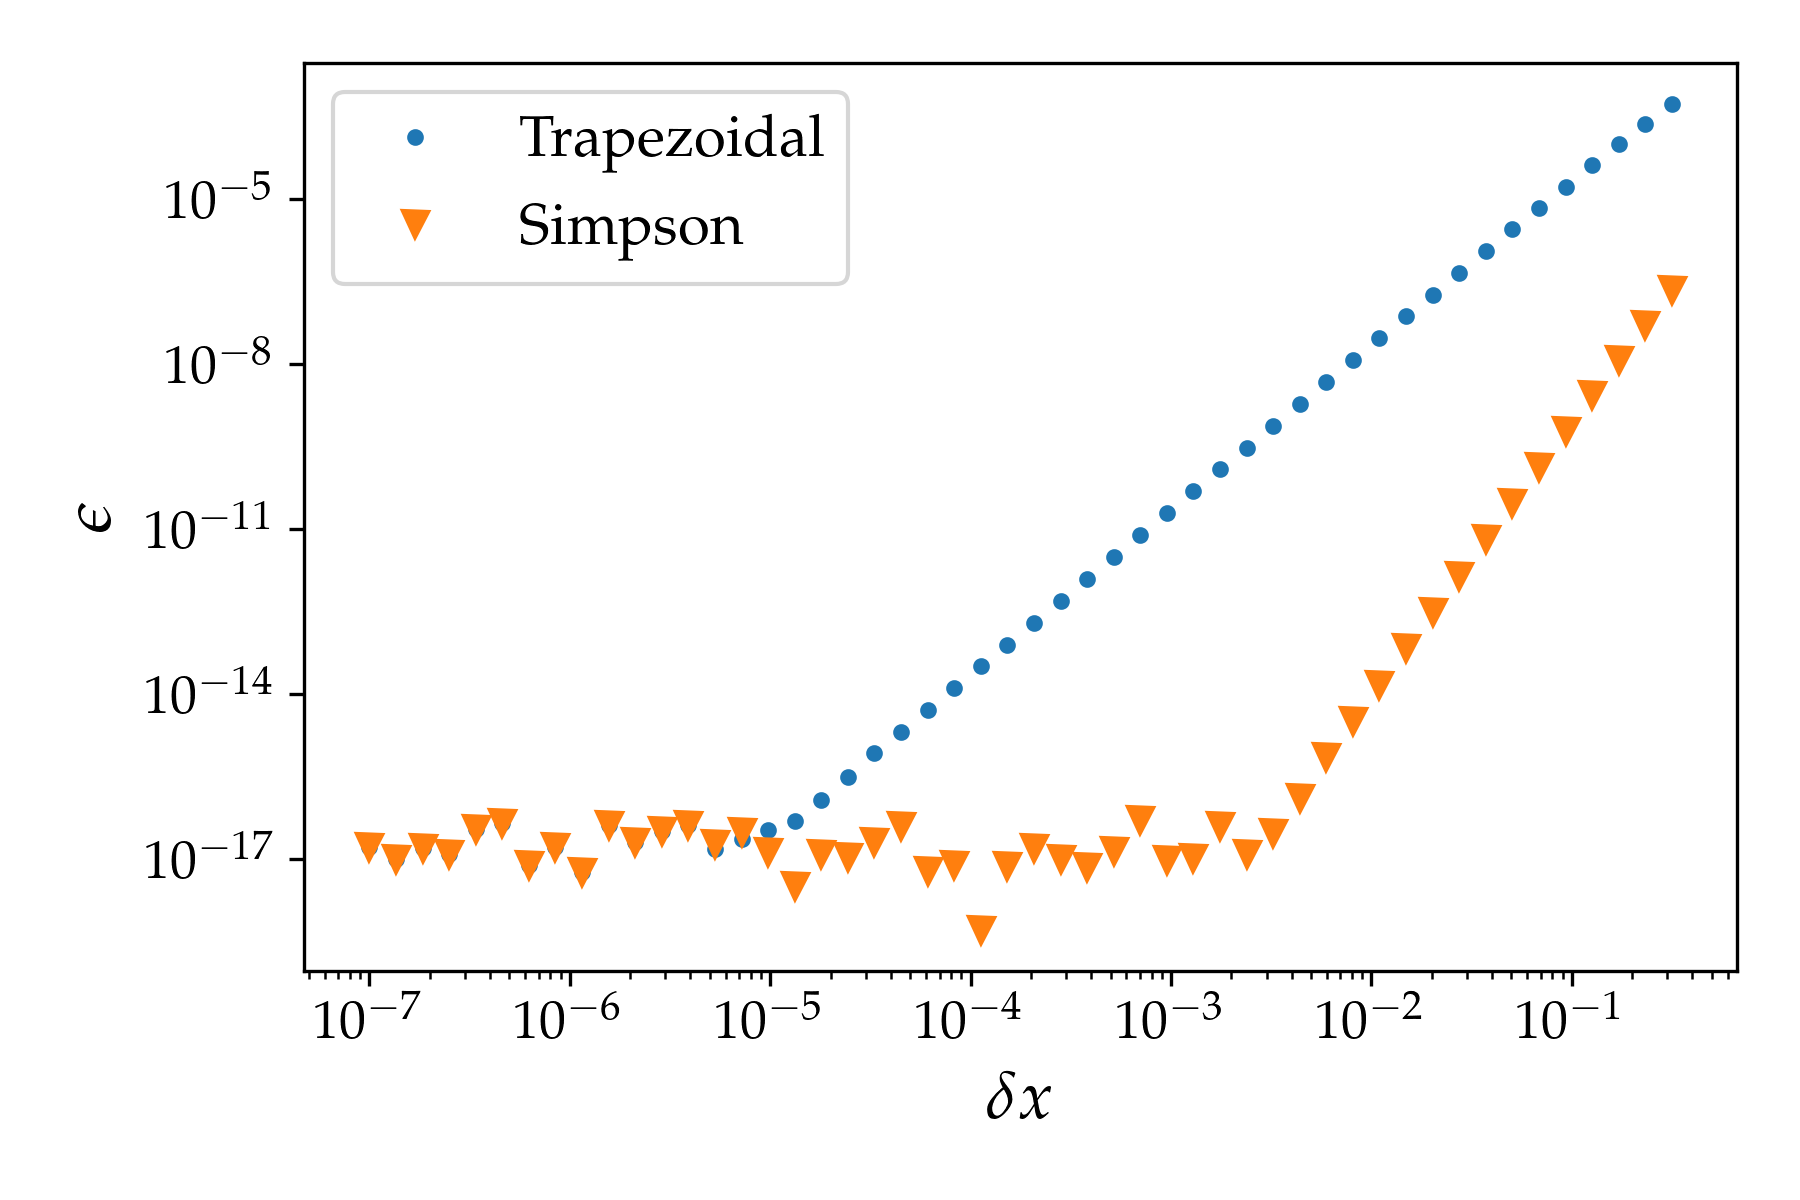
\includegraphics[width=0.8\linewidth]{images/20/confr_locals.png}
    \caption{Confronto tra gli algoritmi in forma locale, in funzione del passo $\delta x$.}
    \label{fig: confr_simp}
\end{figure}

\noindent I fit di seguito verificano i comportamenti che potevamo aspettarci dalla descrizione teorica che è stata fornita precedentemente, cioè dimostrano come la Regola dei trapezi \textit{locale} sia di ordine 3, mentre quella di Simpson di ordine 5.

\begin{figure}[H]
    \centering
    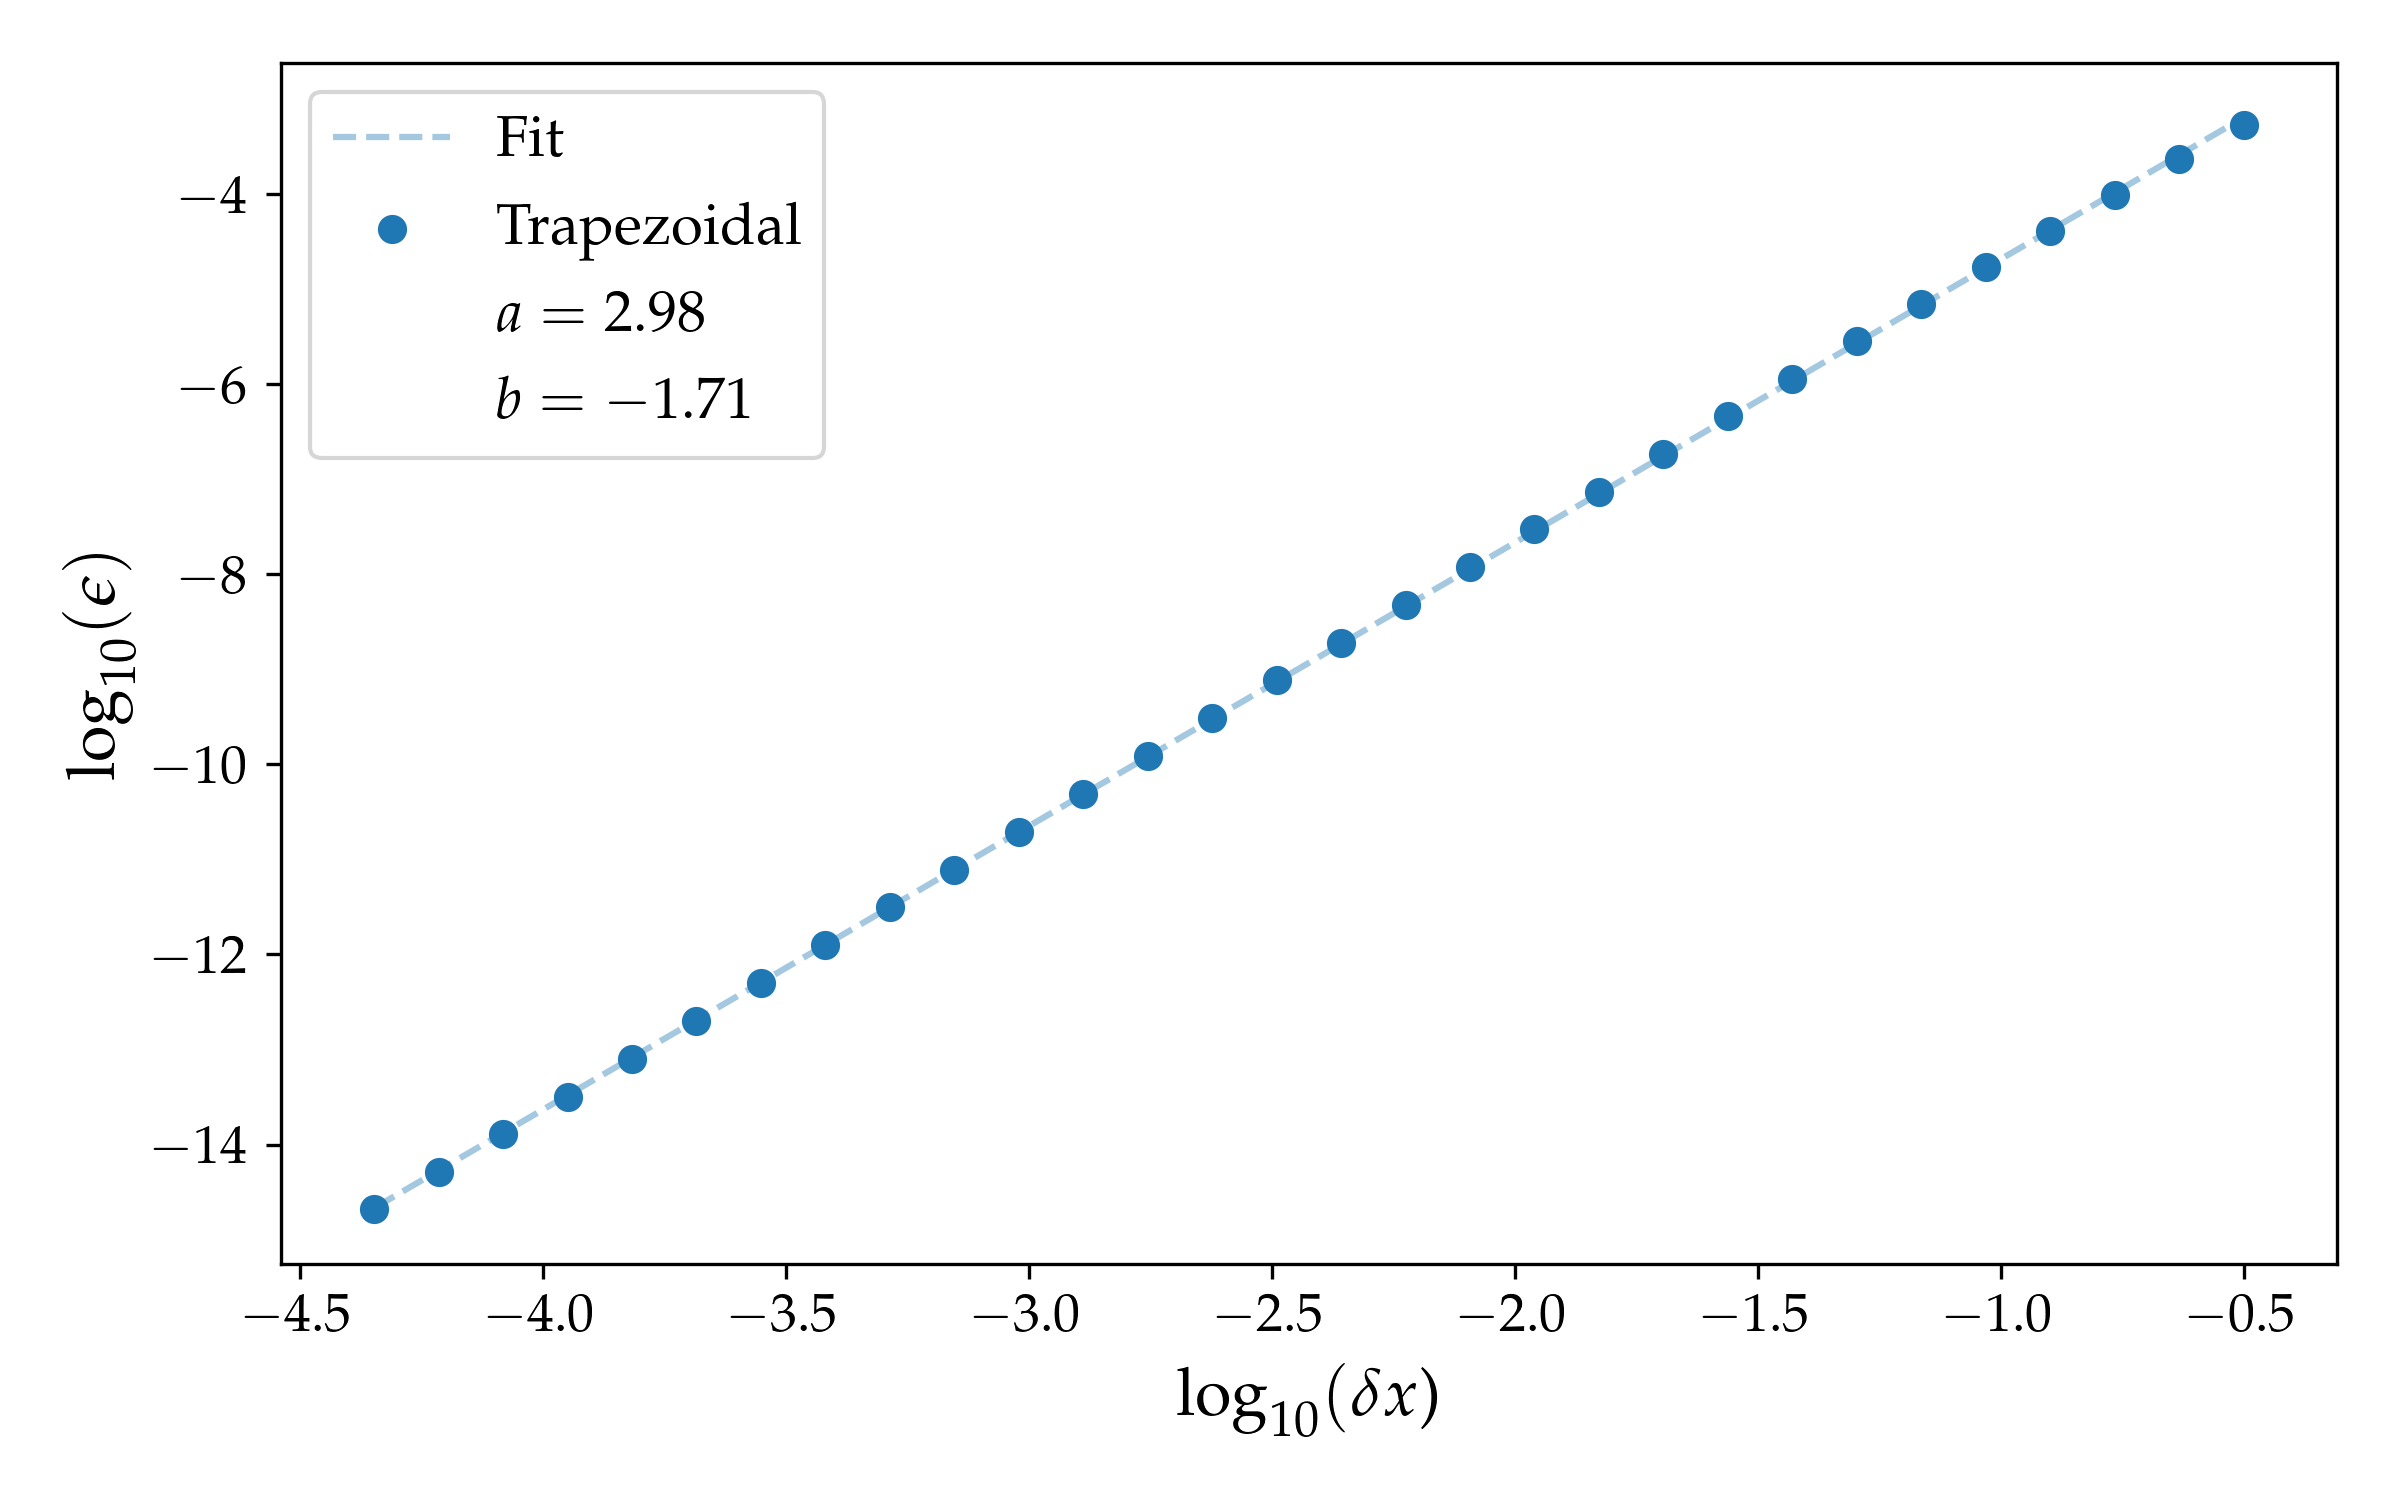
\includegraphics[width=0.8\linewidth]{images/20/Fit_LocTrap.png}
    \caption{Fit lineare (in forma logaritmica) del metodo dei trapezi in funzione dello step $\delta x$.}
    \label{fig: fit_locTrap}
\end{figure}

\begin{figure}[H]
    \centering
    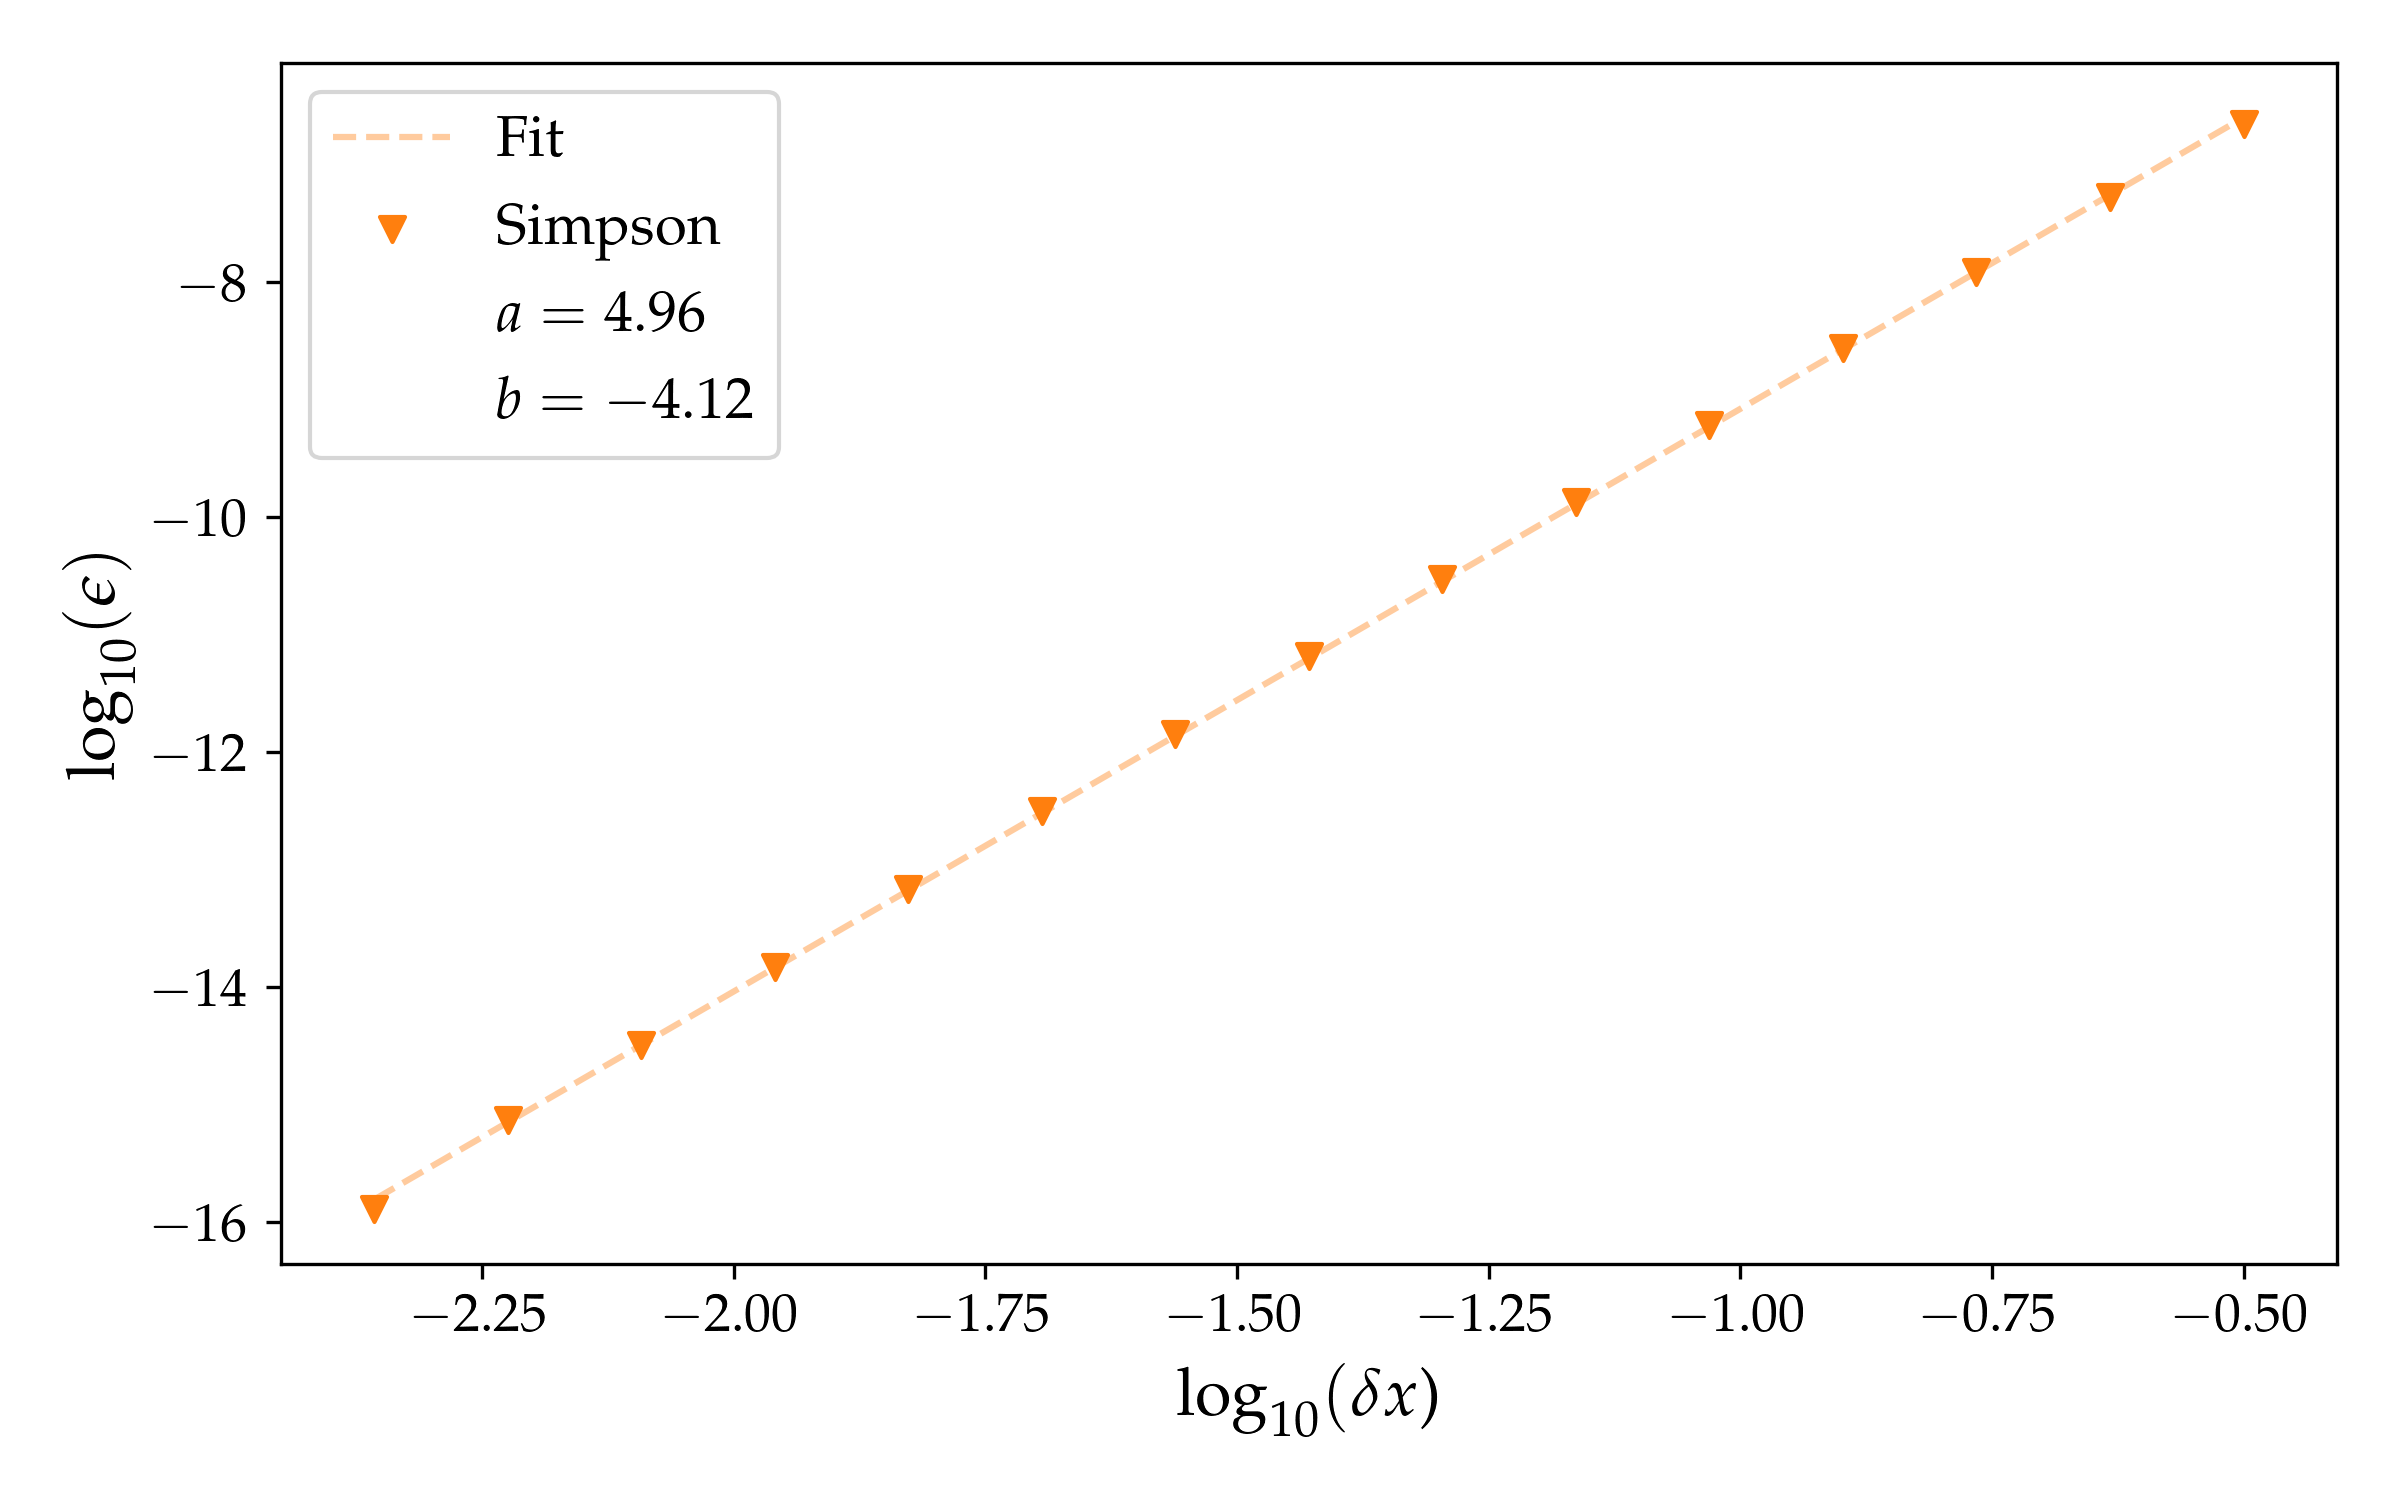
\includegraphics[width=0.8\linewidth]{images/20/Fit_LocSimp.png}
    \caption{Fit lineare (in forma logaritmica) del metodo di Simpson in funzione dello step $\delta x$.}
    \label{fig: fit_locSimp}
\end{figure}

\newpage











\section{Esercizio 8.1.2}
\subsection{Problem Statement}
Utilizzando le regole composite del trapezio e di Simpson, calcolare numericamente l'integrale adimensionale $I$ e verificare l'accuratezza e la convergenza attese del metodo. Per risolvere il problema del limite di integrazione che tende a infinito, considerare l'integrale troncato:

\begin{equation*}
I(x_{\text{max}}) = \int_{0}^{x_{\text{max}}} \frac{x^3}{e^x - 1} \, dx
\end{equation*}

\noindent e, prima di iniziare il calcolo, fornire una stima analitica di $x_{\text{max}}$ tale che l'errore di troncamento sia inferiore alla \textit{machine precision}. Una volta fissato $x_{\text{max}}$, studiare e confrontare lo scaling dei diversi metodi.


\subsection{Premessa Teorica}
In questo problema passiamo ad analizzare gli algoritmi globali dei trapezi e di Simpson, ricordando che entrambi perdono un ordine nello scaling, diventando uno del secondo ordine, l'altro del quarto.

\subsection{Metodi Numerici e Algoritmi}
L'esercizio richiede di risolvere
\begin{equation*}
I = \int_{0}^{+\infty} \frac{x^3}{e^x - 1} \, dx\ \left ( = \frac{\pi^4}{15} \approx 6.49 \right)
\end{equation*}
che è però impossibile, lavorando dal punto di vista numerico: dobbiamo riuscire a isolare su un intervallo finito il nostro campo di azione, cioè escludendo quella coda dell'integrale, per\\ $x_{max} \in (0, +\infty)$:
$$\bar I(x_{\text{max}}) = \int_{x_{\text{max}}}^{\infty} \frac{x^3}{e^x - 1} \, dx \le \varepsilon $$  

\bigskip\noindent
Ho valutato analiticamente $x_{max}$ accettando l'approssimazione che $x_{max}\gg1$: in questo modo
\begin{align*}
e^x -1 &\approx e^x \\
\bar I &\approx \int_{x_{max}}^\infty e^{-x}x^3\ dx > 0\ , \quad x_{max}>0
\end{align*}
cioè la $\Gamma(4, x_{max})$. Risolvo per \textit{IBP} e ottengo:
\[
    \bar I = e^{-x_{max}}(x_{max}^3 + 3x_{max}^2 + 6x_{max} + 6) \le \varepsilon \\
\]
riordinando i termini e semplificando la scrittura:
\begin{align*}
    0 < \bar I / \varepsilon &\le 1 \\
    \log(\bar I/ \varepsilon) &\le 0\\
    \log(\bar I) - \log(\varepsilon) &\le 0
\end{align*}
ridenfinendo infine come
\begin{align*}
    h_{zero}(x) &= \log(\bar I) - \log(\varepsilon)\\
     &=\log(x^3 + 3x^2 + 6x + 6) -  (x + \log(\varepsilon))\\
\end{align*}

\noindent Un algoritmo di ricerca degli zeri, come quelli che abbiamo sviluppato in precedenza, risulta perfetto per la stima necessaria, scegliamo bisezione. Dopo aver studiato $h_{zero}(x)$ in Fig. \ref{fig: zero_res_int}, e avendo scelto un intervallo in cui inizializzare l'algoritmo, troviamo la radice dell'equazione (guardiamo l'uguaglianza e ci ricordiamo della disequazione più avanti).

\noindent La ricerca di $h_{zero}(x) = 0$ restituisce il valore $x_{max} = 48.551645373827725$.

\begin{figure}[H]
    \centering
    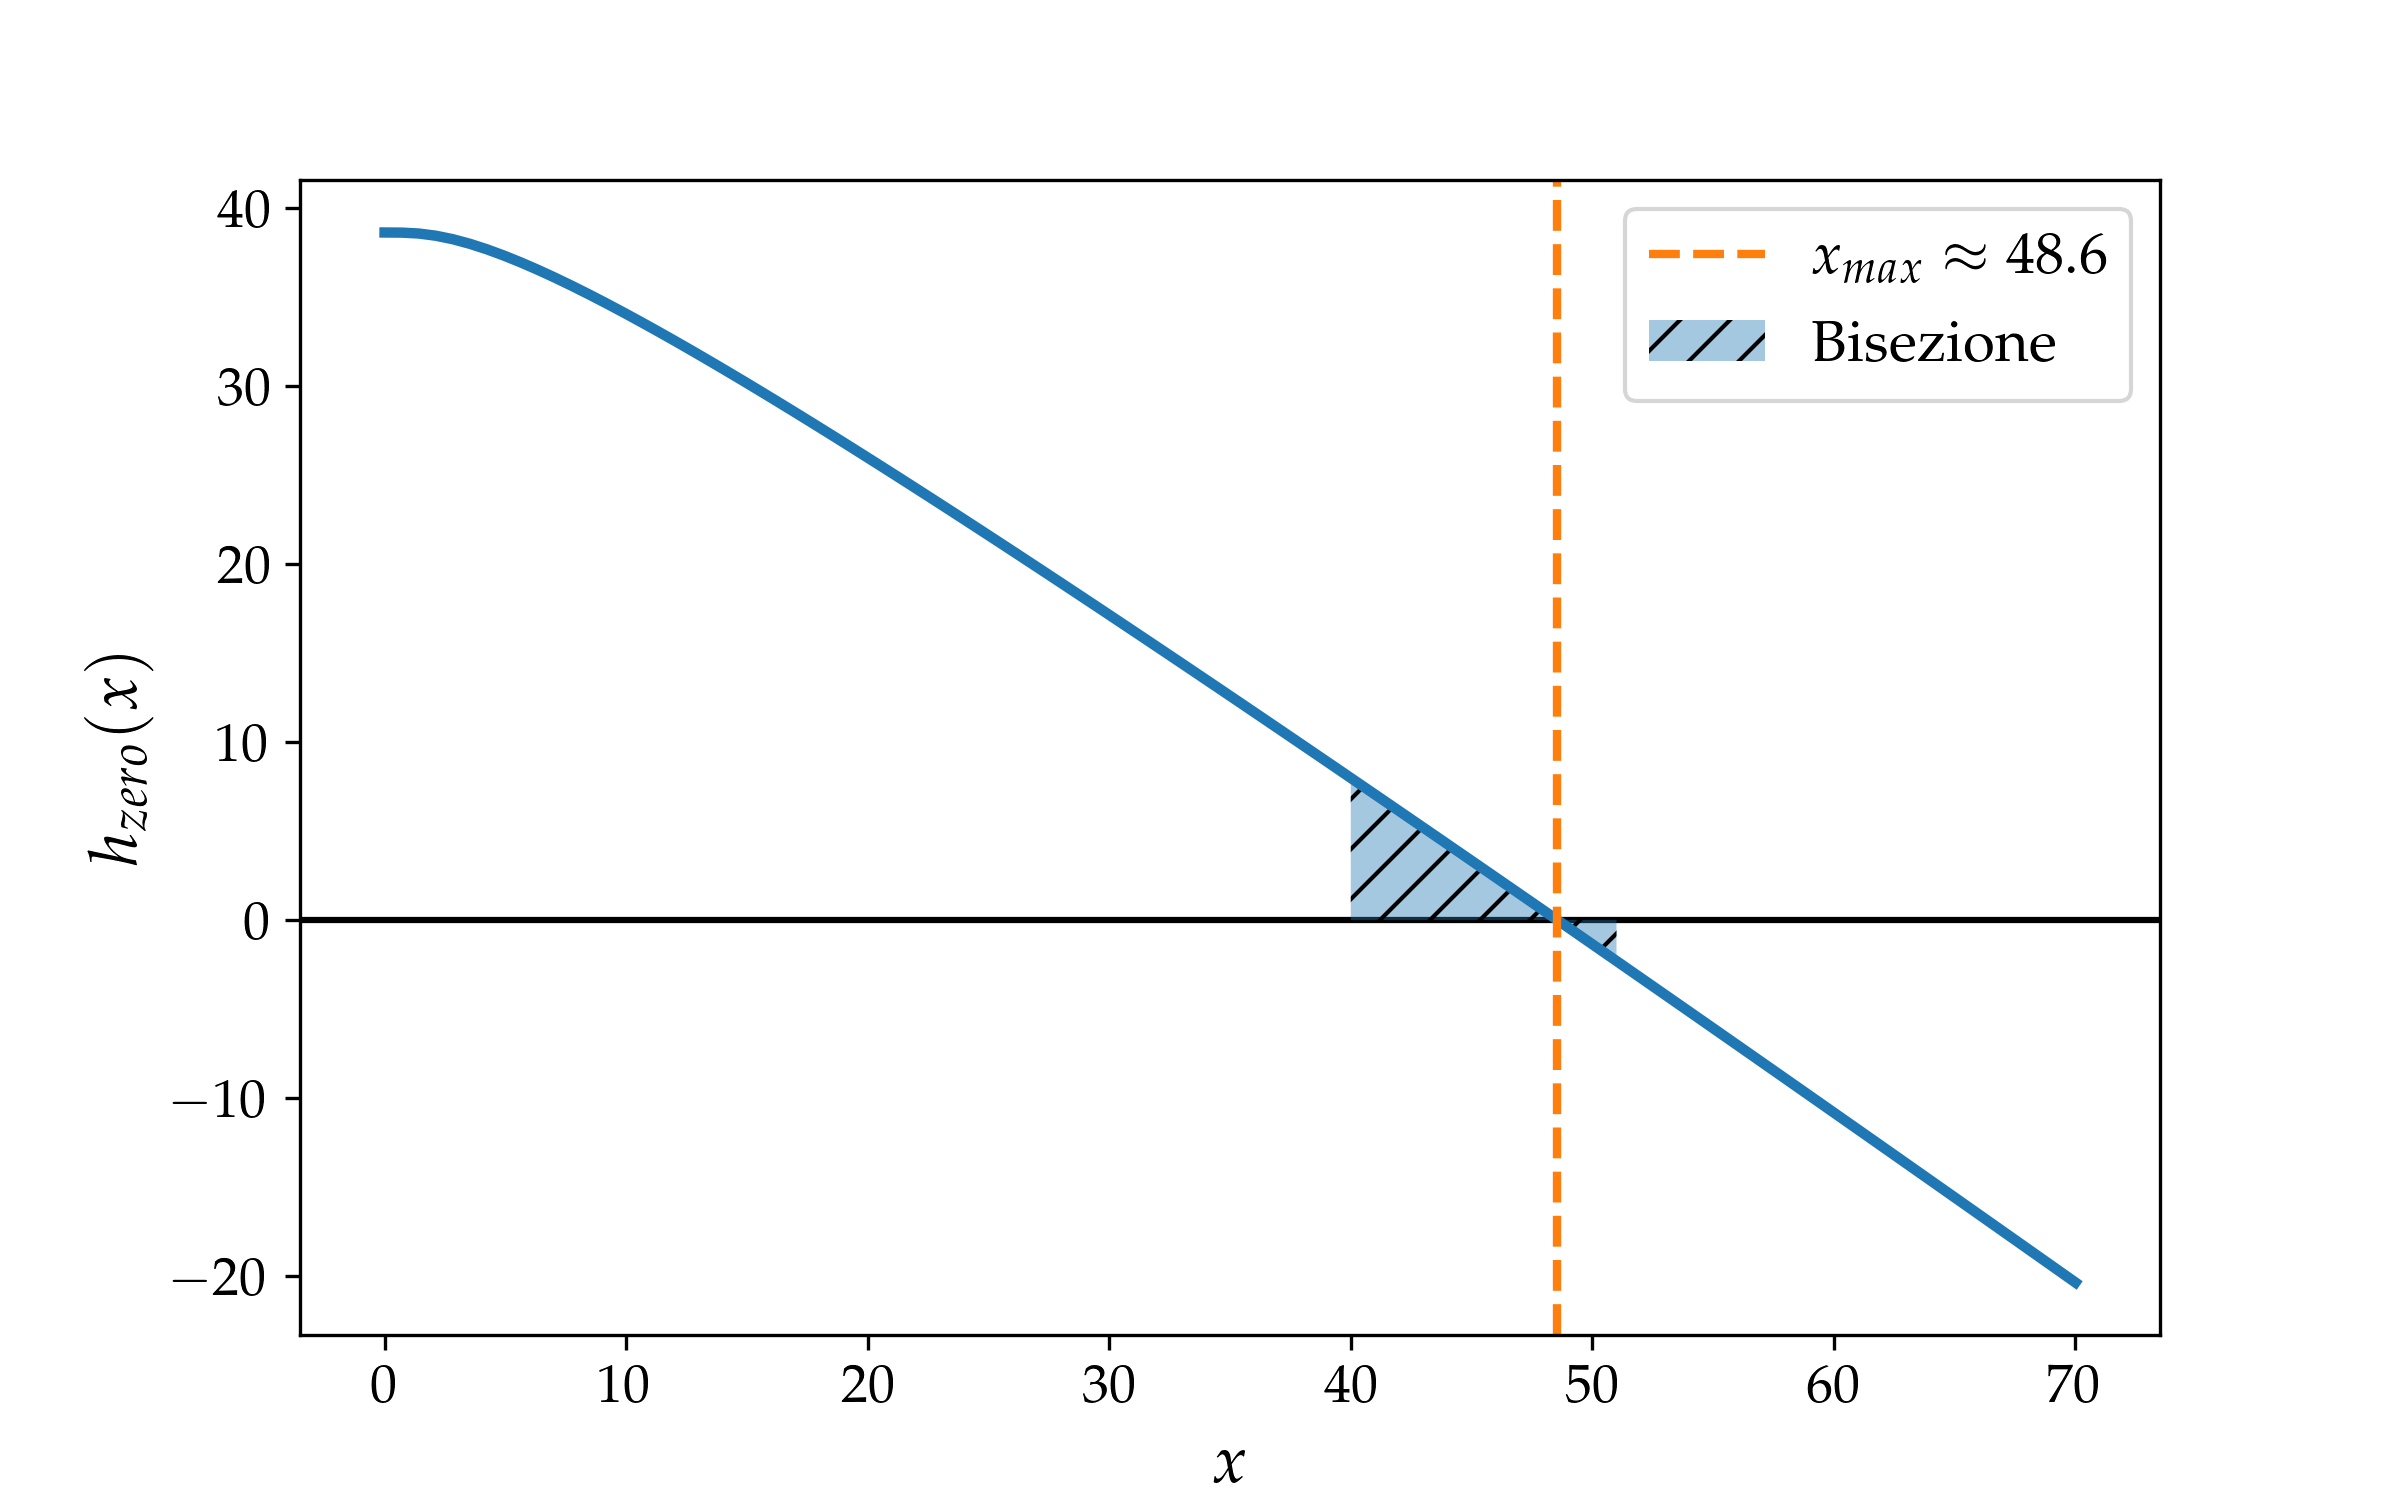
\includegraphics[width=0.8\linewidth]{images/20/zero_res.png}
    \caption{Ricerca degli zeri sulla funzione $g_{zero}(x)$ con l'algoritmo di Bisezione: è stato scelto l'intervallo $x\in [20, 50]$.}
    \label{fig: zero_res_int}
\end{figure}

\noindent La condizione approssimata è che si ottiene è quindi che $x_{max} > 49$. In Fig. \ref{fig: x_int_conf} la verifica del nostro calcolo, valutando l'andamento della funzione integrale:
\[
F(x) = \int_0^x f(t)\ dt
\]
Infine segue un ultimo confronto riepilogativo, per il confronto anche con il metodo dei trapezi e per valutare brevemente l'approssimazione necessaria che facciamo per $x=0 \to x =10^{-9}$.

\begin{elegantcode}
a = 1e-09
b = 48.551645373827725

True = 6.493939402266828
residual = 3.333333333333334e-28


Trapezi:

I_t = 6.4939394022668235
leftover = 1.0000000734565665e-16
diff = 4.440892098500626e-15


Simpson:

I_s = 6.493939402266805
leftover = 9.996869800764608e-17
diff = 2.3092638912203256e-14
\end{elegantcode}


\begin{figure}[H]
    \centering
    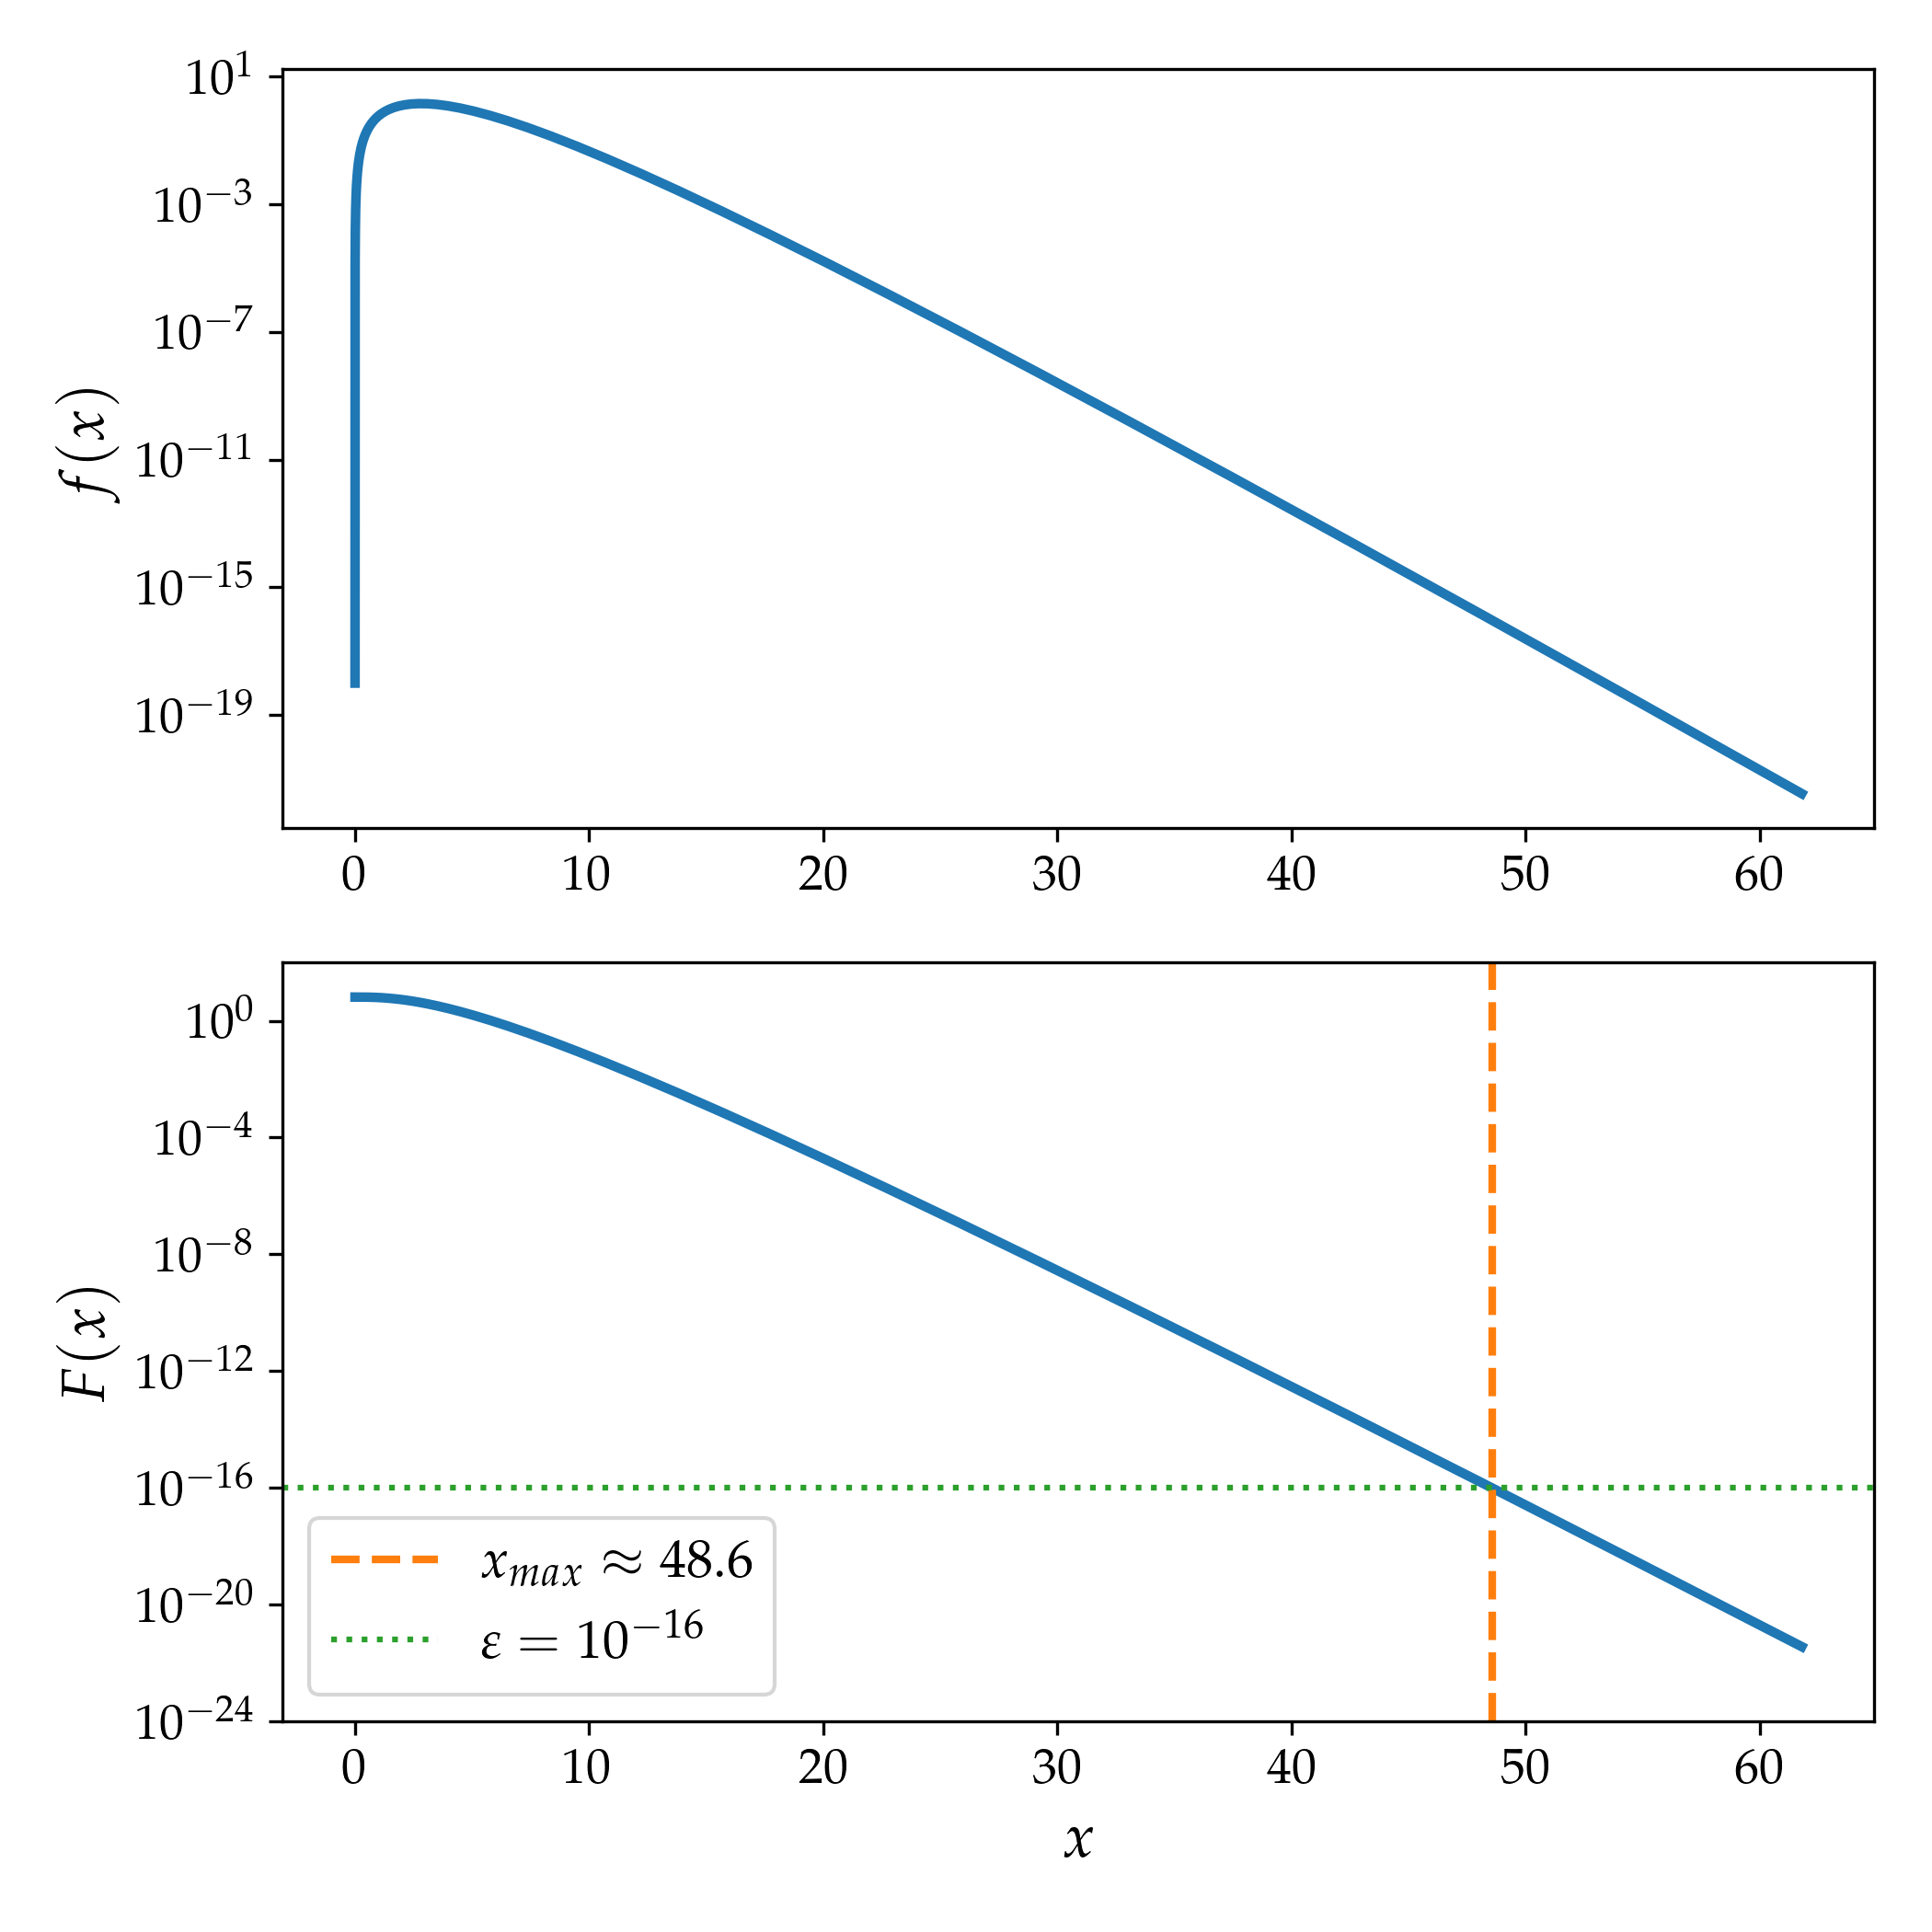
\includegraphics[width=0.7\linewidth]{images/20/x_int_conf.png}
    \caption{Andamento delle funzioni $f(x),F(x)$. La \textit{treshold} fissata a $\varepsilon=10^{-16}$ è coerente con il valore che abbiamo appena determinato.}
    \label{fig: x_int_conf}
\end{figure}


\subsection{Risultati e Discussione}

Si mostrano di seguito i risultati del confronto dei due metodi, Fig. \ref{fig: glob_conf}, e dei fit sui singoli, Fig. \ref{fig: fit_trap_glob} e \ref{fig: fit_simp_glob}. Per i fit si seleziona solo la parte più a destra del confronto, escludendo le sezioni in cui si forma il plateau relativo alla \textit{machine precision}.

\noindent È lampante osservare dal primo grafico, ma dai fit abbiamo la conferma rigorosa, che se il metodo di Simpson si comporta come ci attendevamo di rilevare, non fa lo stesso quello dei trapezi, che produce un andamento a convergenza del quarto ordine. Questo commento non contraddice ciò che abbiamo precedentemente affermato, però mette in luce un fenomeno numerico che deve star avvenendo per aumentare l'ordine di convergenza nel metodo.

\medskip\noindent
L'andamento numerico osservato suggerisce una superconvergenza del metodo dei trapezi per questa specifica funzione.\\
Il metodo dei trapezi ha errore locale 

\begin{equation*}
    \epsilon_{L, i} = -\frac{1}{12} \delta x^3 f''(x_i) -\frac{1}{24} \delta x^4 f'''(x_i) + O(\delta x^5) \,.
\end{equation*}
passando all'errore totale (cioè relativo al metodo in forma composta), che è l'accumulazione degli errori locali:

$$\epsilon_G = \sum \epsilon_{L,i} = -\frac{1}{12}\delta x^2 \sum f''(x_i)\delta x - \frac{1}{24}\delta x^3 \sum f'''(x_i)\delta x + O(\delta x^4)$$

sviluppando ulteriormente fino al quarto ordine e ricordando:

$$\sum g(x_i)\delta x = \int_a^b g(x)dx - \frac{\delta x}{2} (g(b) - g(a)) + O(\delta x^2)$$

Applicandolo alle nostre derivate:

\begin{align*}
    \sum f''(x_i)\delta x &= \int_a^b f''(x)dx - \frac{\delta x}{2} \left( f'' (b)-f'' (a) \right)  + O(\delta x^2)  \\
    &= (f'(b) - f'(a)) - \frac{\delta x}{2} \left( f'' (b)-f'' (a) \right)  + O(\delta x^2)\\
    \sum f'''(x_i) \delta x &= \int_a^b f'''(x)dx = f''(b) - f''(a) + O(\delta x)
\end{align*}

\begin{align*}
    \epsilon_G =& -\frac{1}{12}\delta x^2 (f'(b) - f'(a)) + \frac{1}{24}\delta x^3 (f''(b) - f''(a)) - \frac{1}{24}\delta x^3 (f''(b) - f''(a)) + O(\delta x^4)\\
    =& -\frac{1}{12}\delta x^2 (f'(b) - f'(a))   + O(\delta x^4)
\end{align*}

\noindent sapendo che per la funzione specifica con cui stiamo lavorando vale che la derivata prima è nulla in entrambi gli estremi $a, b$ (Fig. \ref{fig: der_conf}), concludiamo che $\epsilon = O(\delta x^4)$.

\noindent L'algoritmo è quindi dell'ordine 4. Questo tipo di fenomeno viene definito superconvergenza e rappresenta l'occasione di ricorrere ad algoritmi in generale meno performativi, ma ottimi per alcune loro caratteristiche per problemi specifici.

\begin{figure}[H]
    \centering
    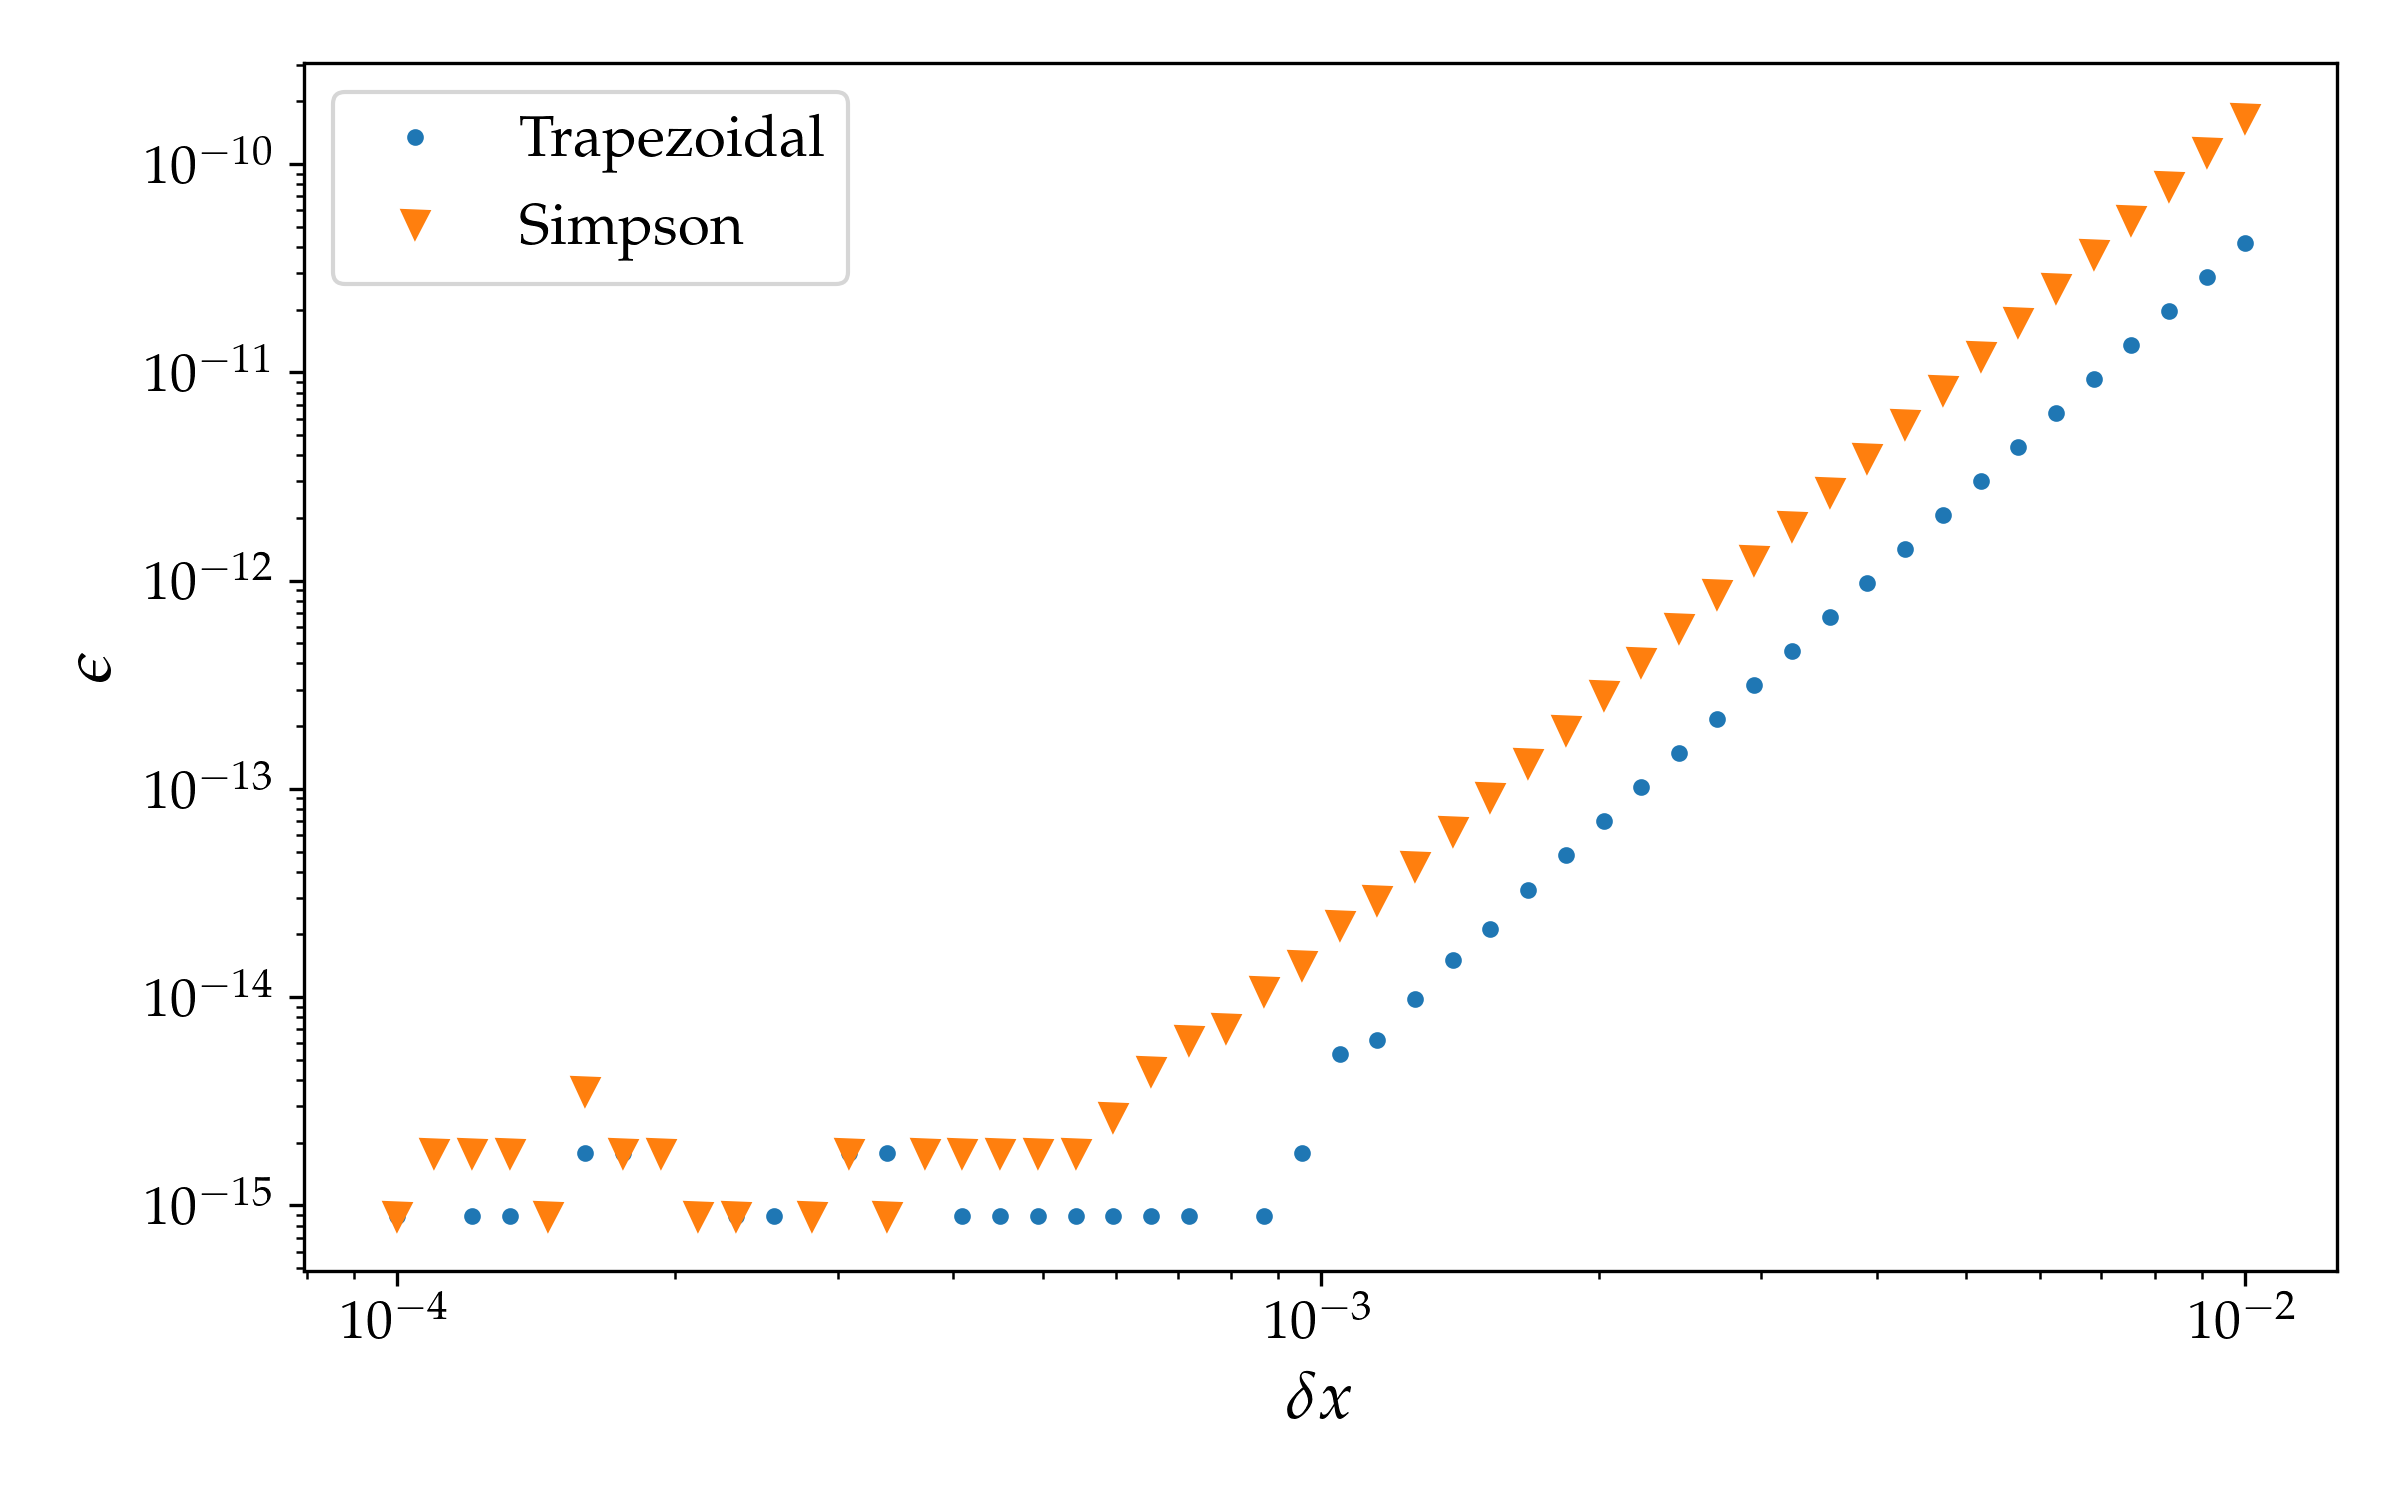
\includegraphics[width=0.8\linewidth]{images/20/confr_glob.png}
    \caption{Confronto fra gli andamenti dei due metodi per integrazione numerica. Entrambi raggiungono il plateau di \textit{machine precision} da cui non è più possibile osservare l'ordine di convergenza.}
    \label{fig: glob_conf}
\end{figure}

\begin{figure}[H]
    \centering
    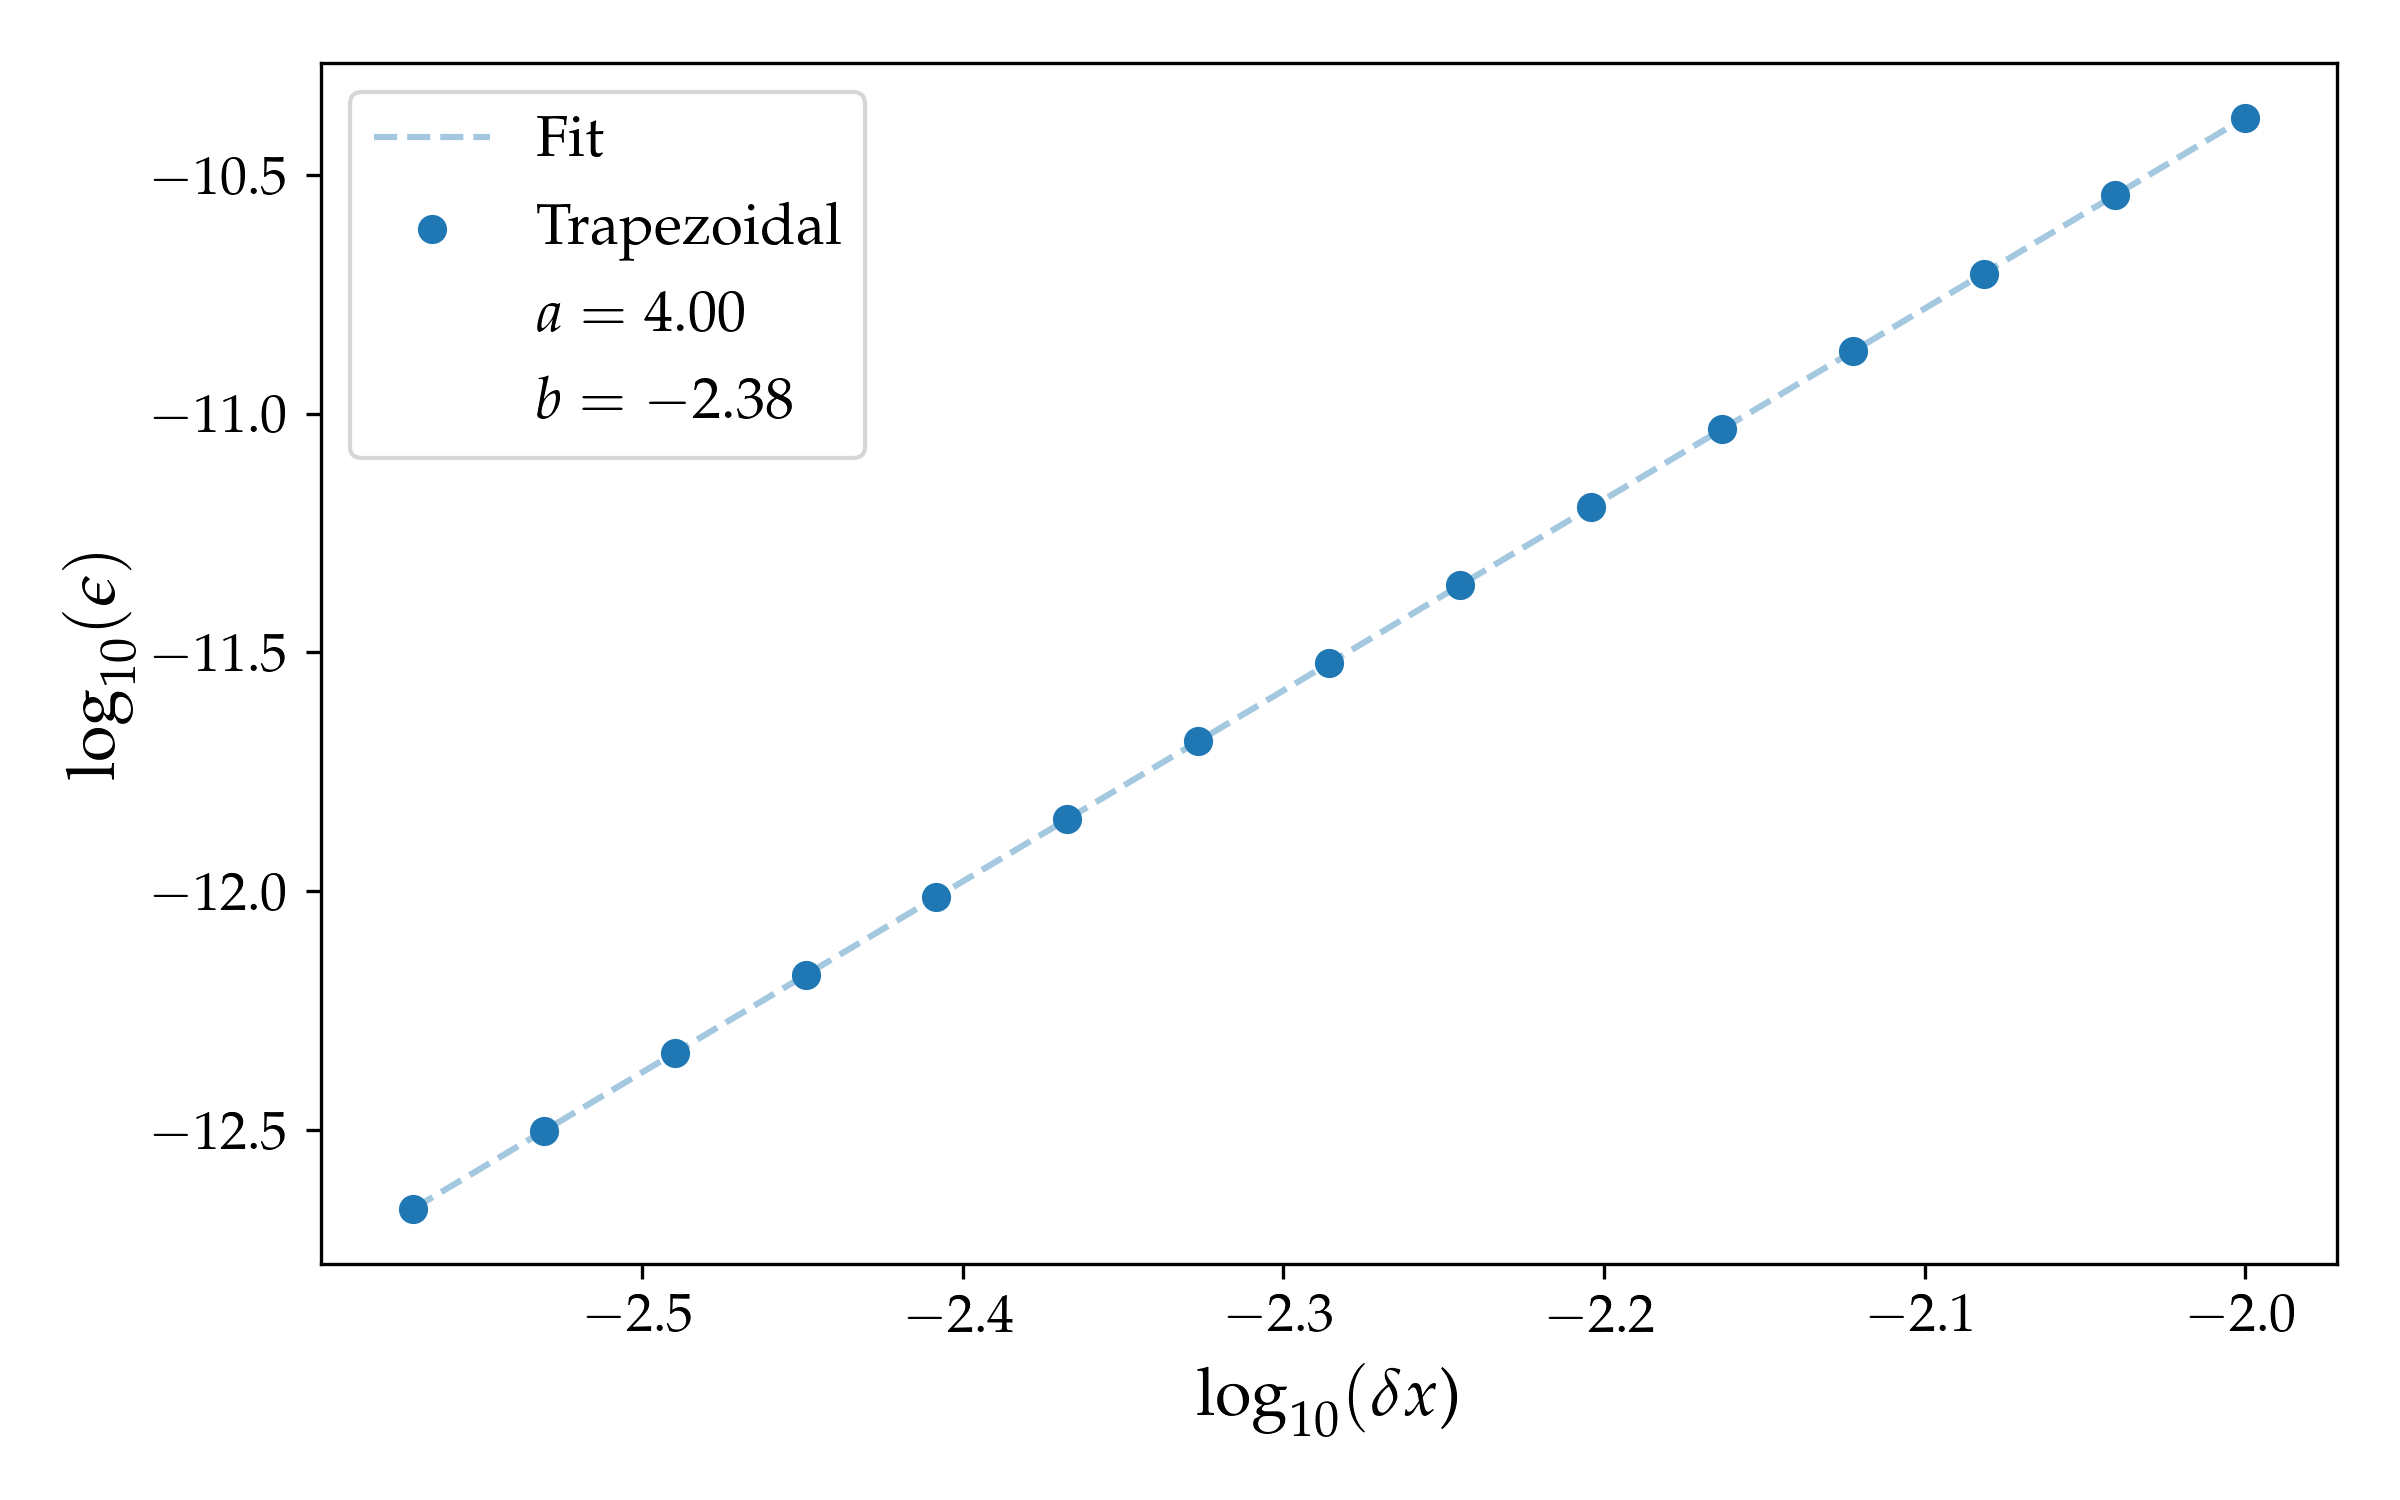
\includegraphics[width=0.8\linewidth]{images/20/Fit_gl_trap.png}
    \caption{Fit sulla Regola dei trapezi composta in funzione del passo $\delta x$.}
    \label{fig: fit_trap_glob}
\end{figure}

\begin{figure}[H]
    \centering
    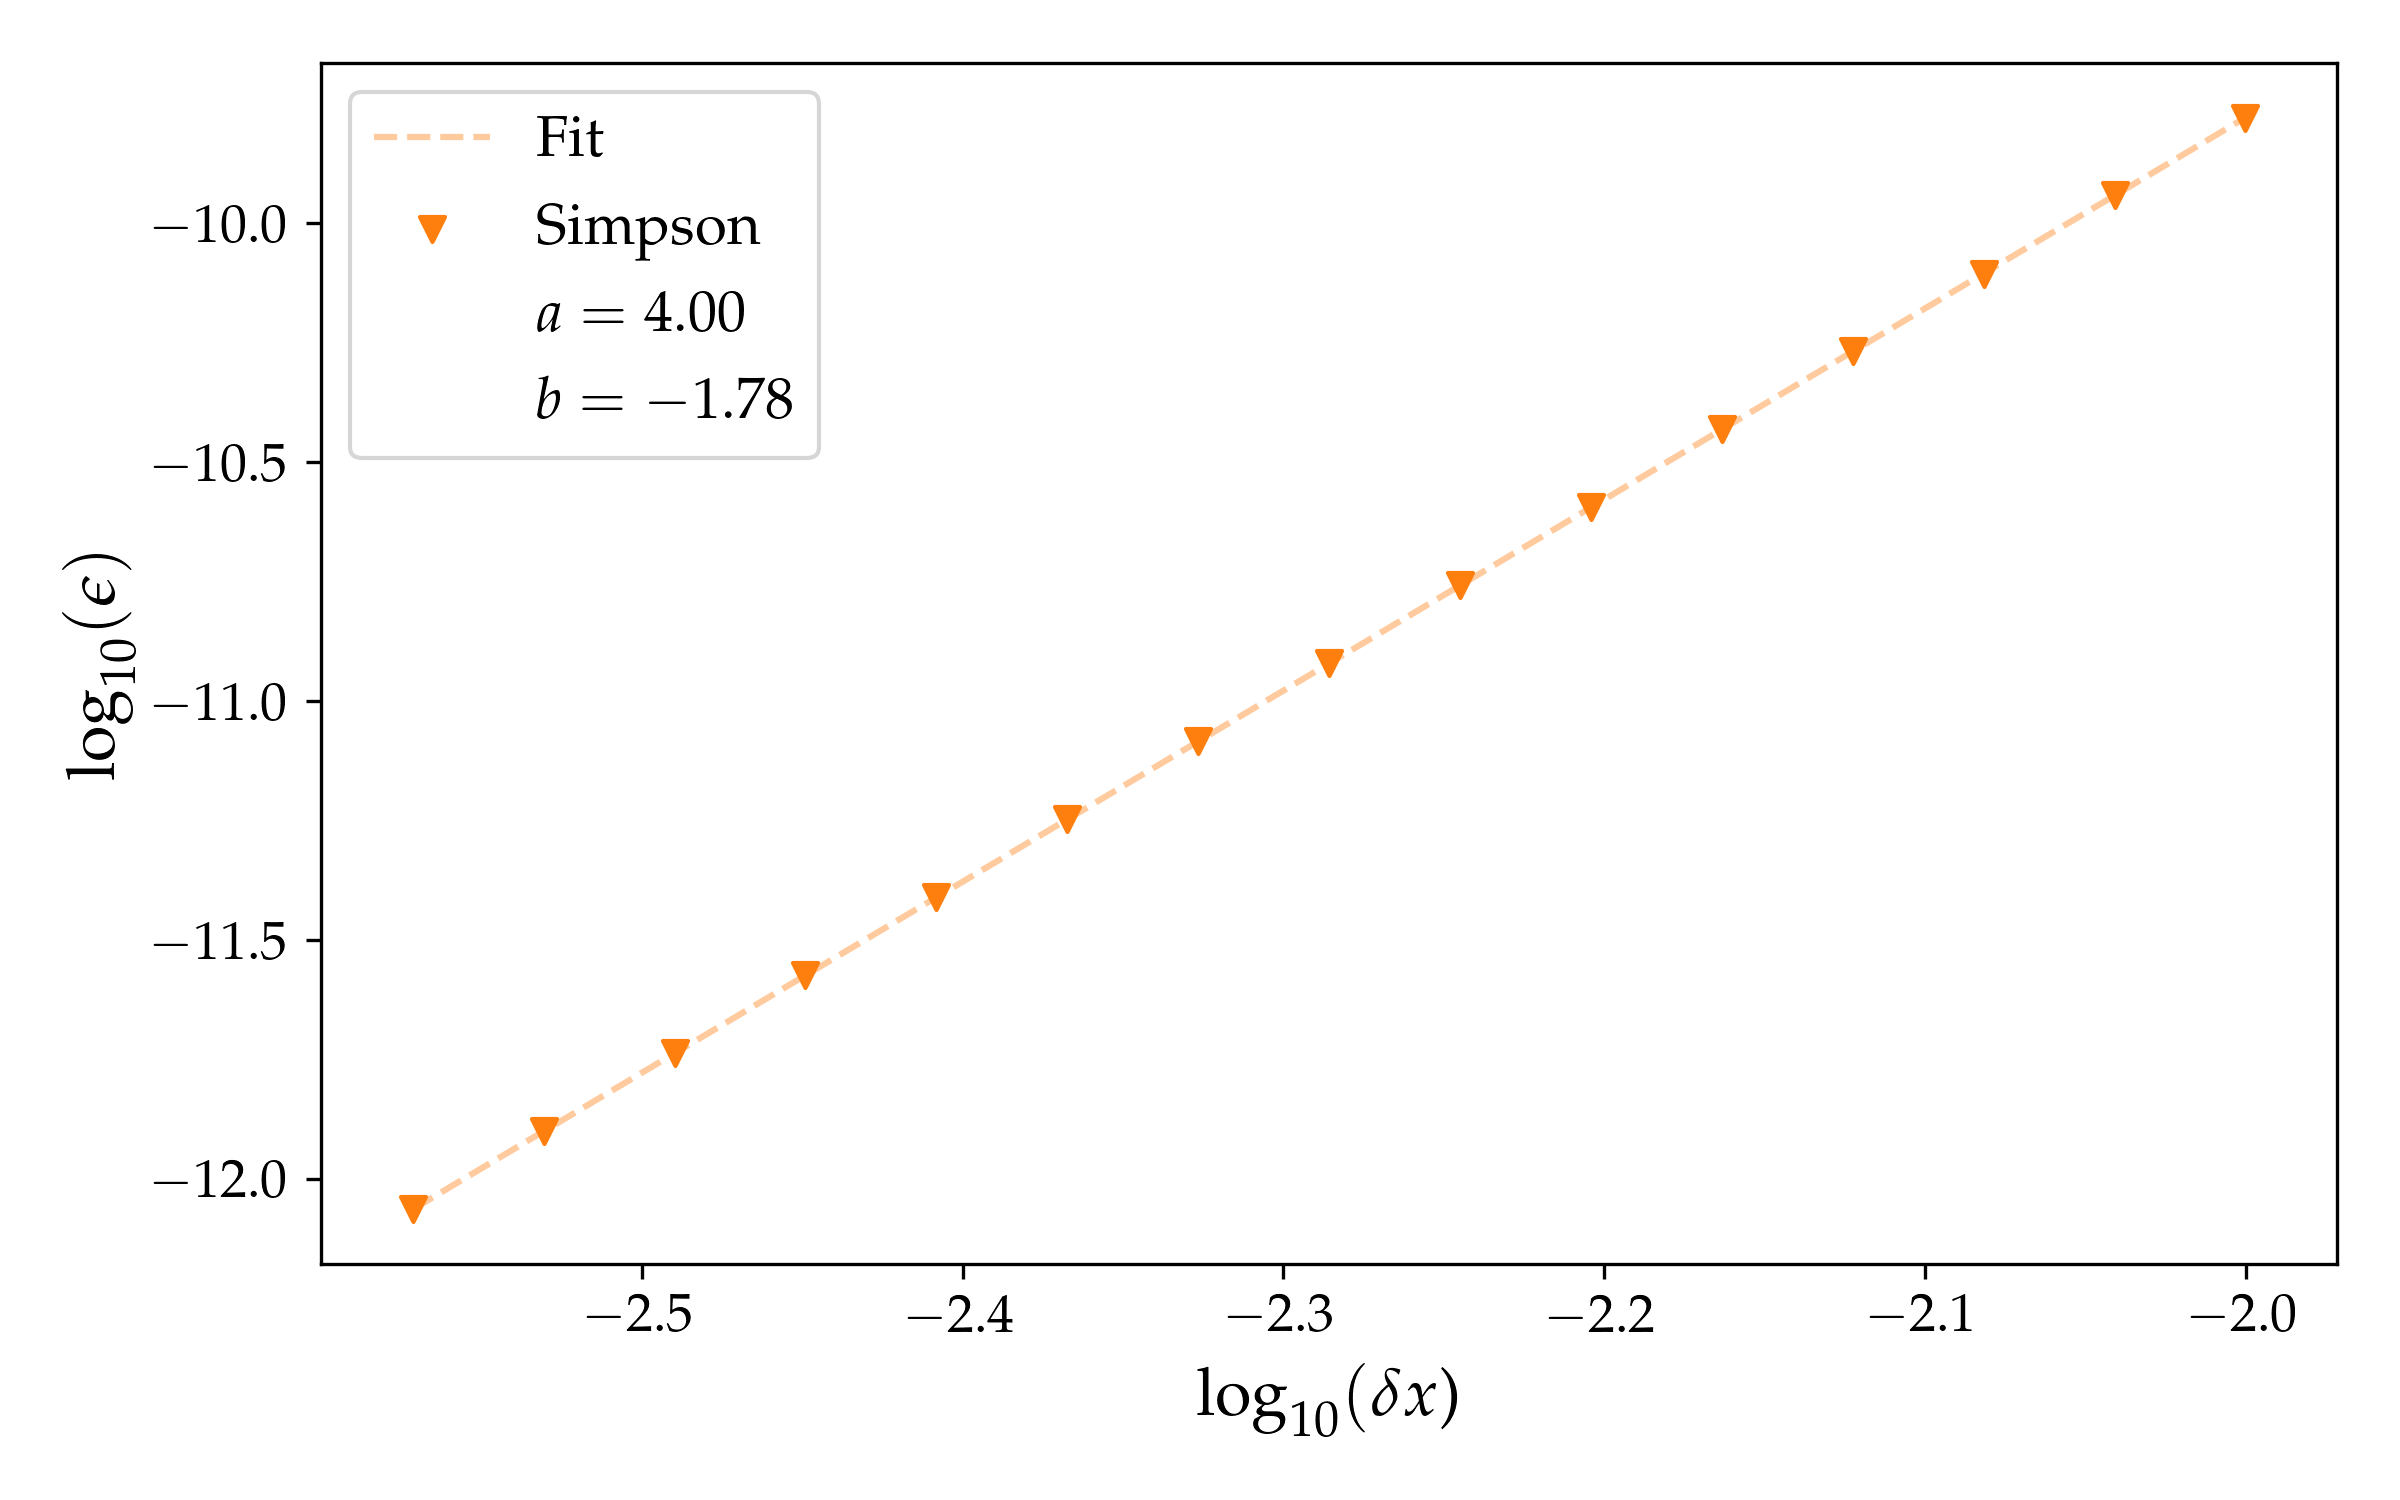
\includegraphics[width=0.8\linewidth]{images/20/Fit_gl_simp.png}
    \caption{Fit sulla Regola di Simpson composta in funzione del passo $\delta x$.}
    \label{fig: fit_simp_glob}
\end{figure}

\begin{figure}[H]
    \centering
    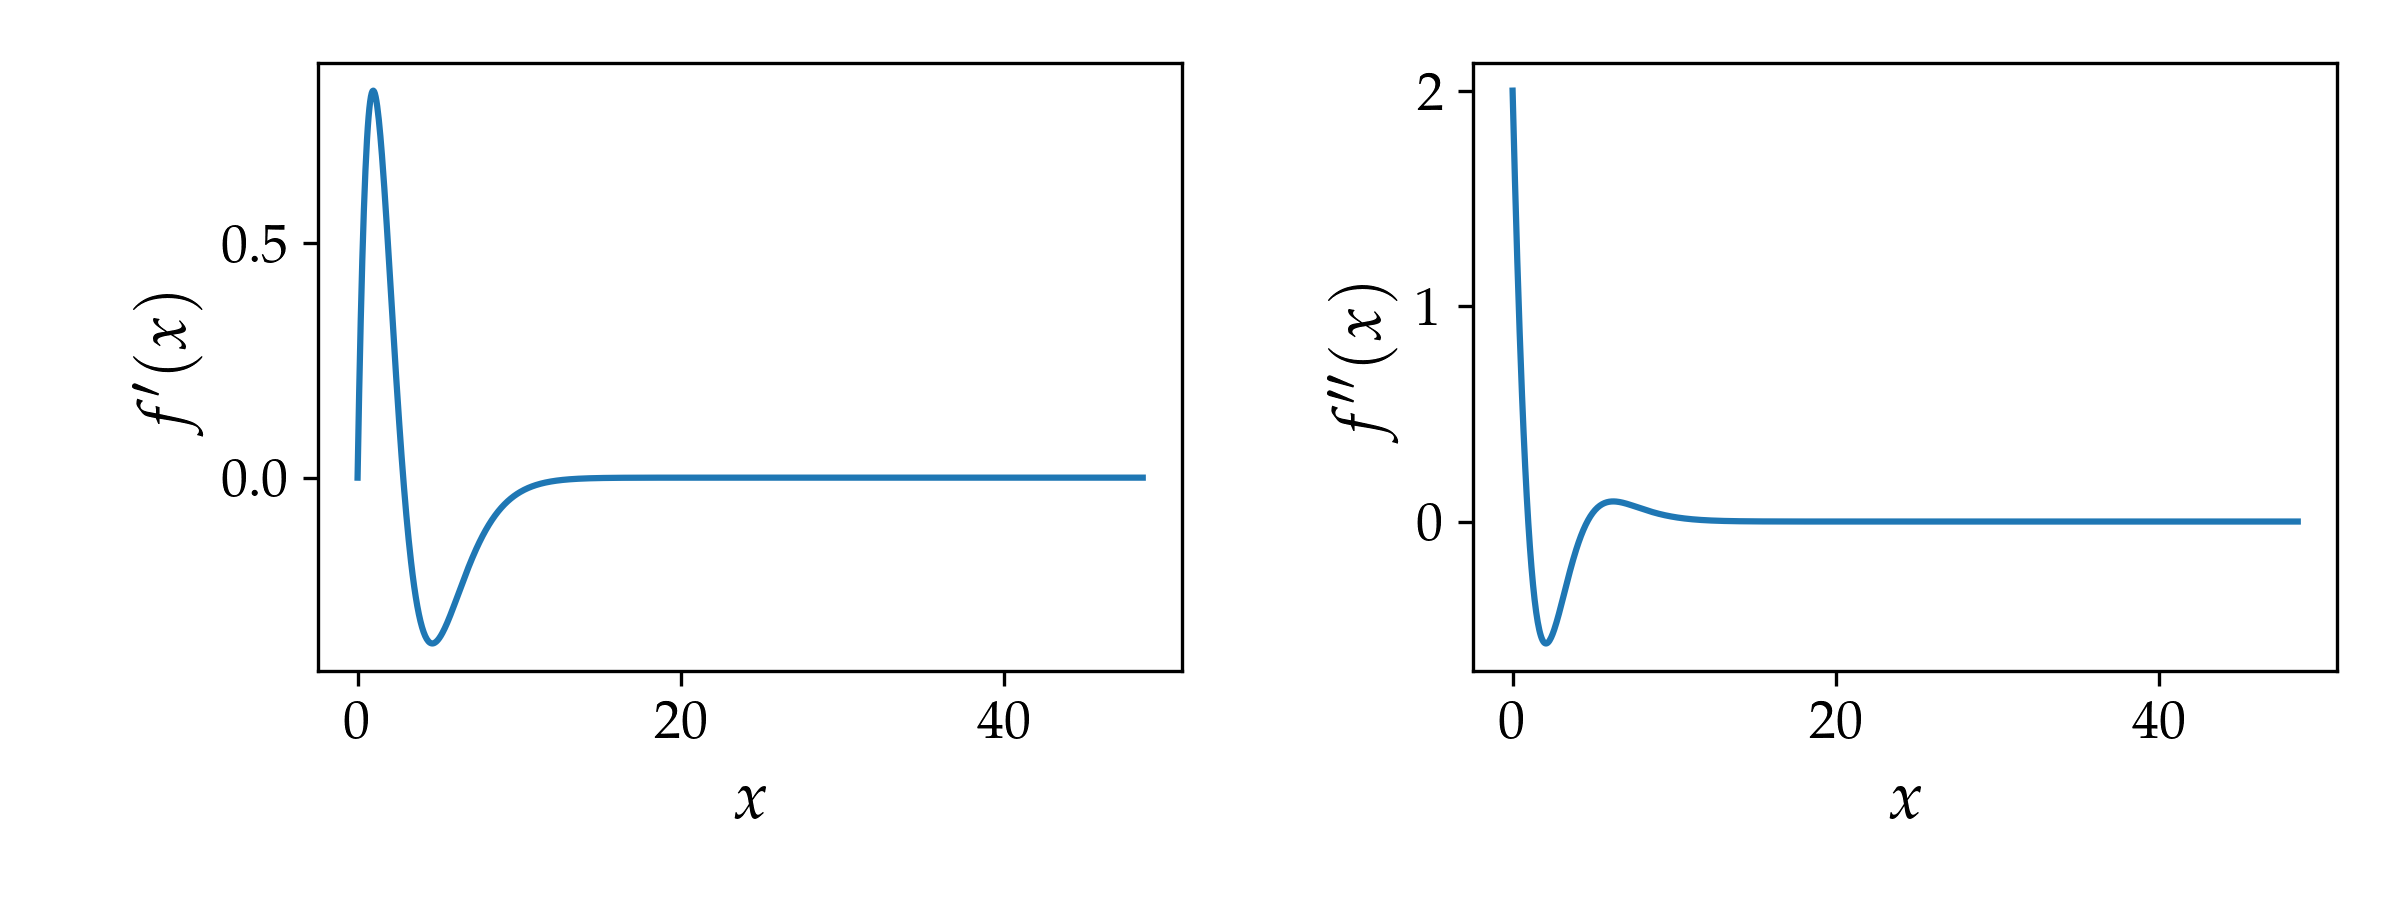
\includegraphics[width=\linewidth]{images/20/der_conf.png}
    \caption{Visualizzazione e confronto della derivata prima e seconda della funzione. Si può verificare che la prima si annulla agli estremi: $f'(0) =f'(x_{max}) = 0$.}
    \label{fig: der_conf}
\end{figure}

\newpage

















\section{Esercizio 8.2.1}
\subsection{Problem Statement}
Si consideri l'integrale
\[
\int_{0}^{1} \frac{4}{1 + x^2} \, dx = \pi
\]
e si studi l'accuratezza della soluzione in funzione di $\Delta x$ per la regola dei trapezi, la regola di Simpson e la quadratura di Gauss-Legendre a 2 punti. Utilizzando la conoscenza analitica dell'andamento dell'errore, si predica (per tutti i metodi) per quale valore di $N$ l'errore assoluto è pari a $10^{-6}$ e lo si verifichi con i dati.


\subsection{Premessa Teorica}
Se per gli algoritmi che abbiamo discusso in precedenza, per l'integrazione numerica, la suddivisione dell'intervallo era uniforme, possiamo scegliere questi punti in maniera più oculata.\\
Non tutti gli intervalli contribuiscono allo stesso modo al calcolo; l'introduzione di pesi e posizioni ben specifiche permette di aumentare la precisione e diminuire il numero di valutazioni della funzione.

\subsection{Metodi Numerici e Algoritmi}

La quadratura di Gauss-Legendre a 2 punti è una tecnica di integrazione numerica che ottimizza la posizione dei nodi di campionamento per massimizzare il grado di precisione del metodo, superando le limitazioni dei metodi a punti equidistanti come quelli di Newton-Cotes.

Per un dato intervallo $[x_0, x_0 + \delta x]$, l'integrale è approssimato come:
\begin{equation*}
    \int_{x_{0}}^{x_{0}+\delta x}dx~f(x) \approx \frac{\delta x}{2}[f(x_{+})+f(x_{-})]
\end{equation*}
dove i nodi di valutazione sono definiti dalla relazione:
\begin{equation*}
    x_{\pm} = x_0 + \frac{\delta x}{2} \left( 1 \pm \frac{1}{\sqrt{3}} \right)
\end{equation*}

Il metodo presenta la caratteristica di utilizzare solo due valutazioni della funzione: garantisce un'accuratezza paragonabile alla regola di Simpson, ma richiedendo un numero inferiore di valutazioni ($2$ rispetto a $3$), con un vantaggio computazionale del $33\%$.

\noindent L'algoritmo deriva dalla scelta dei nodi come radici del polinomio di Legendre di secondo grado, $P_2(x) = \frac{1}{2}(3x^2 - 1)$, la cui proprietà di ortogonalità garantisce l'annullamento dei termini di ordine superiore nell'espansione di Taylor dell'integrando.

\newpage
\subsection{Risultati e Discussione}

In primis valutiamo con i differenti metodi il valore dell'integrale, verificando la validità degli stessi; si controlla anche l'errore assoluto rispetto al valore vero di $I=\pi$.


\begin{elegantcode}
a = 0
b = 1
True = 3.141592653589793


Trapezi:

I_t = 3.141592653573126
diff = 1.66671121348827e-11


Simpson:

I_s = 3.141592653589794
diff = 8.881784197001252e-16


Gauss-Legendre: 

I_g = 3.1415926535897936
diff = 4.440892098500626e-16
\end{elegantcode}


\bigskip\noindent
Seguendo le indicazioni della consegna, desideriamo studiare e predire, per ciascun metodo, per quale valore di $N$ l'errore si assesti sotto la soglia di $\epsilon=10^{-6}$.

\begin{figure}[H]
    \centering
    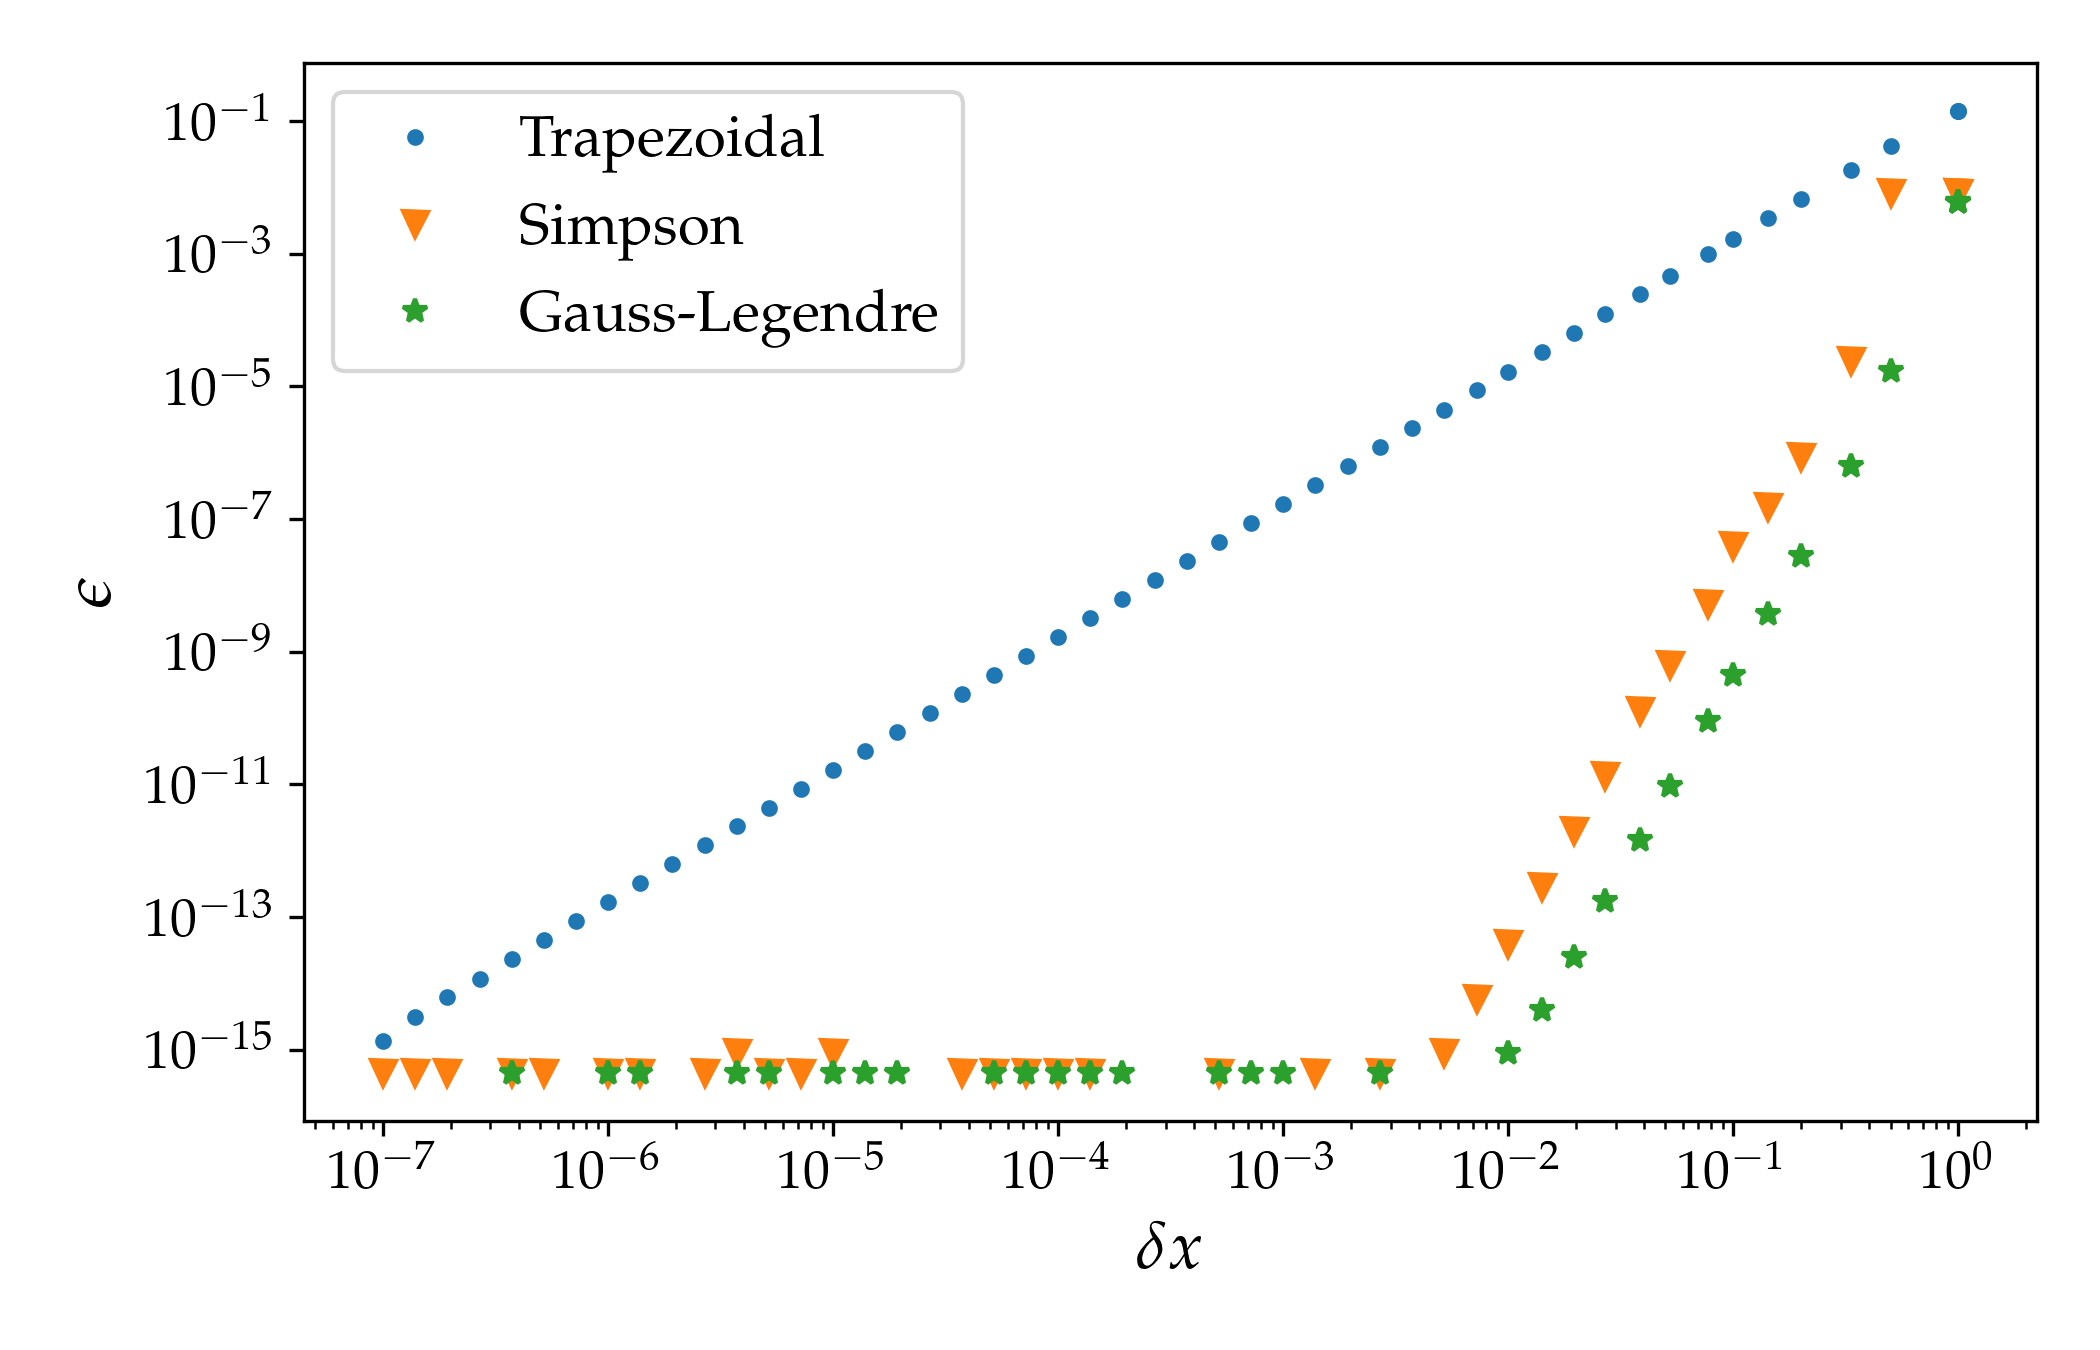
\includegraphics[width=0.8\linewidth]{images/21/conf_3mth.png}
    \caption{Confronto della convergenza tra i diversi metodi, in funzione di $\delta x$, intervallo uniforme in cui sezioniamo $I=[0,1]$.}
    \label{fig: conv_int_dx}
\end{figure}

\noindent In generale abbiamo già fatto alcune considerazioni sulla convergenza dei tre metodi, affermando che quello dei trapezi ha convergenza quadratica, mentre gli altri due quartica; in questo caso commentiamo i risultati del fit che viene fatto studiando l'errore degli algoritmi in funzione del passo $\delta x\in [10^{-7}, 1]$ (cioè proprio il loro \textit{scaling}).\\
Seguono Fig. \ref{fig: fit_trap_6} - \ref{fig: fit_Gauss_leg} per confronto.

\begin{figure}[H]
    \centering
    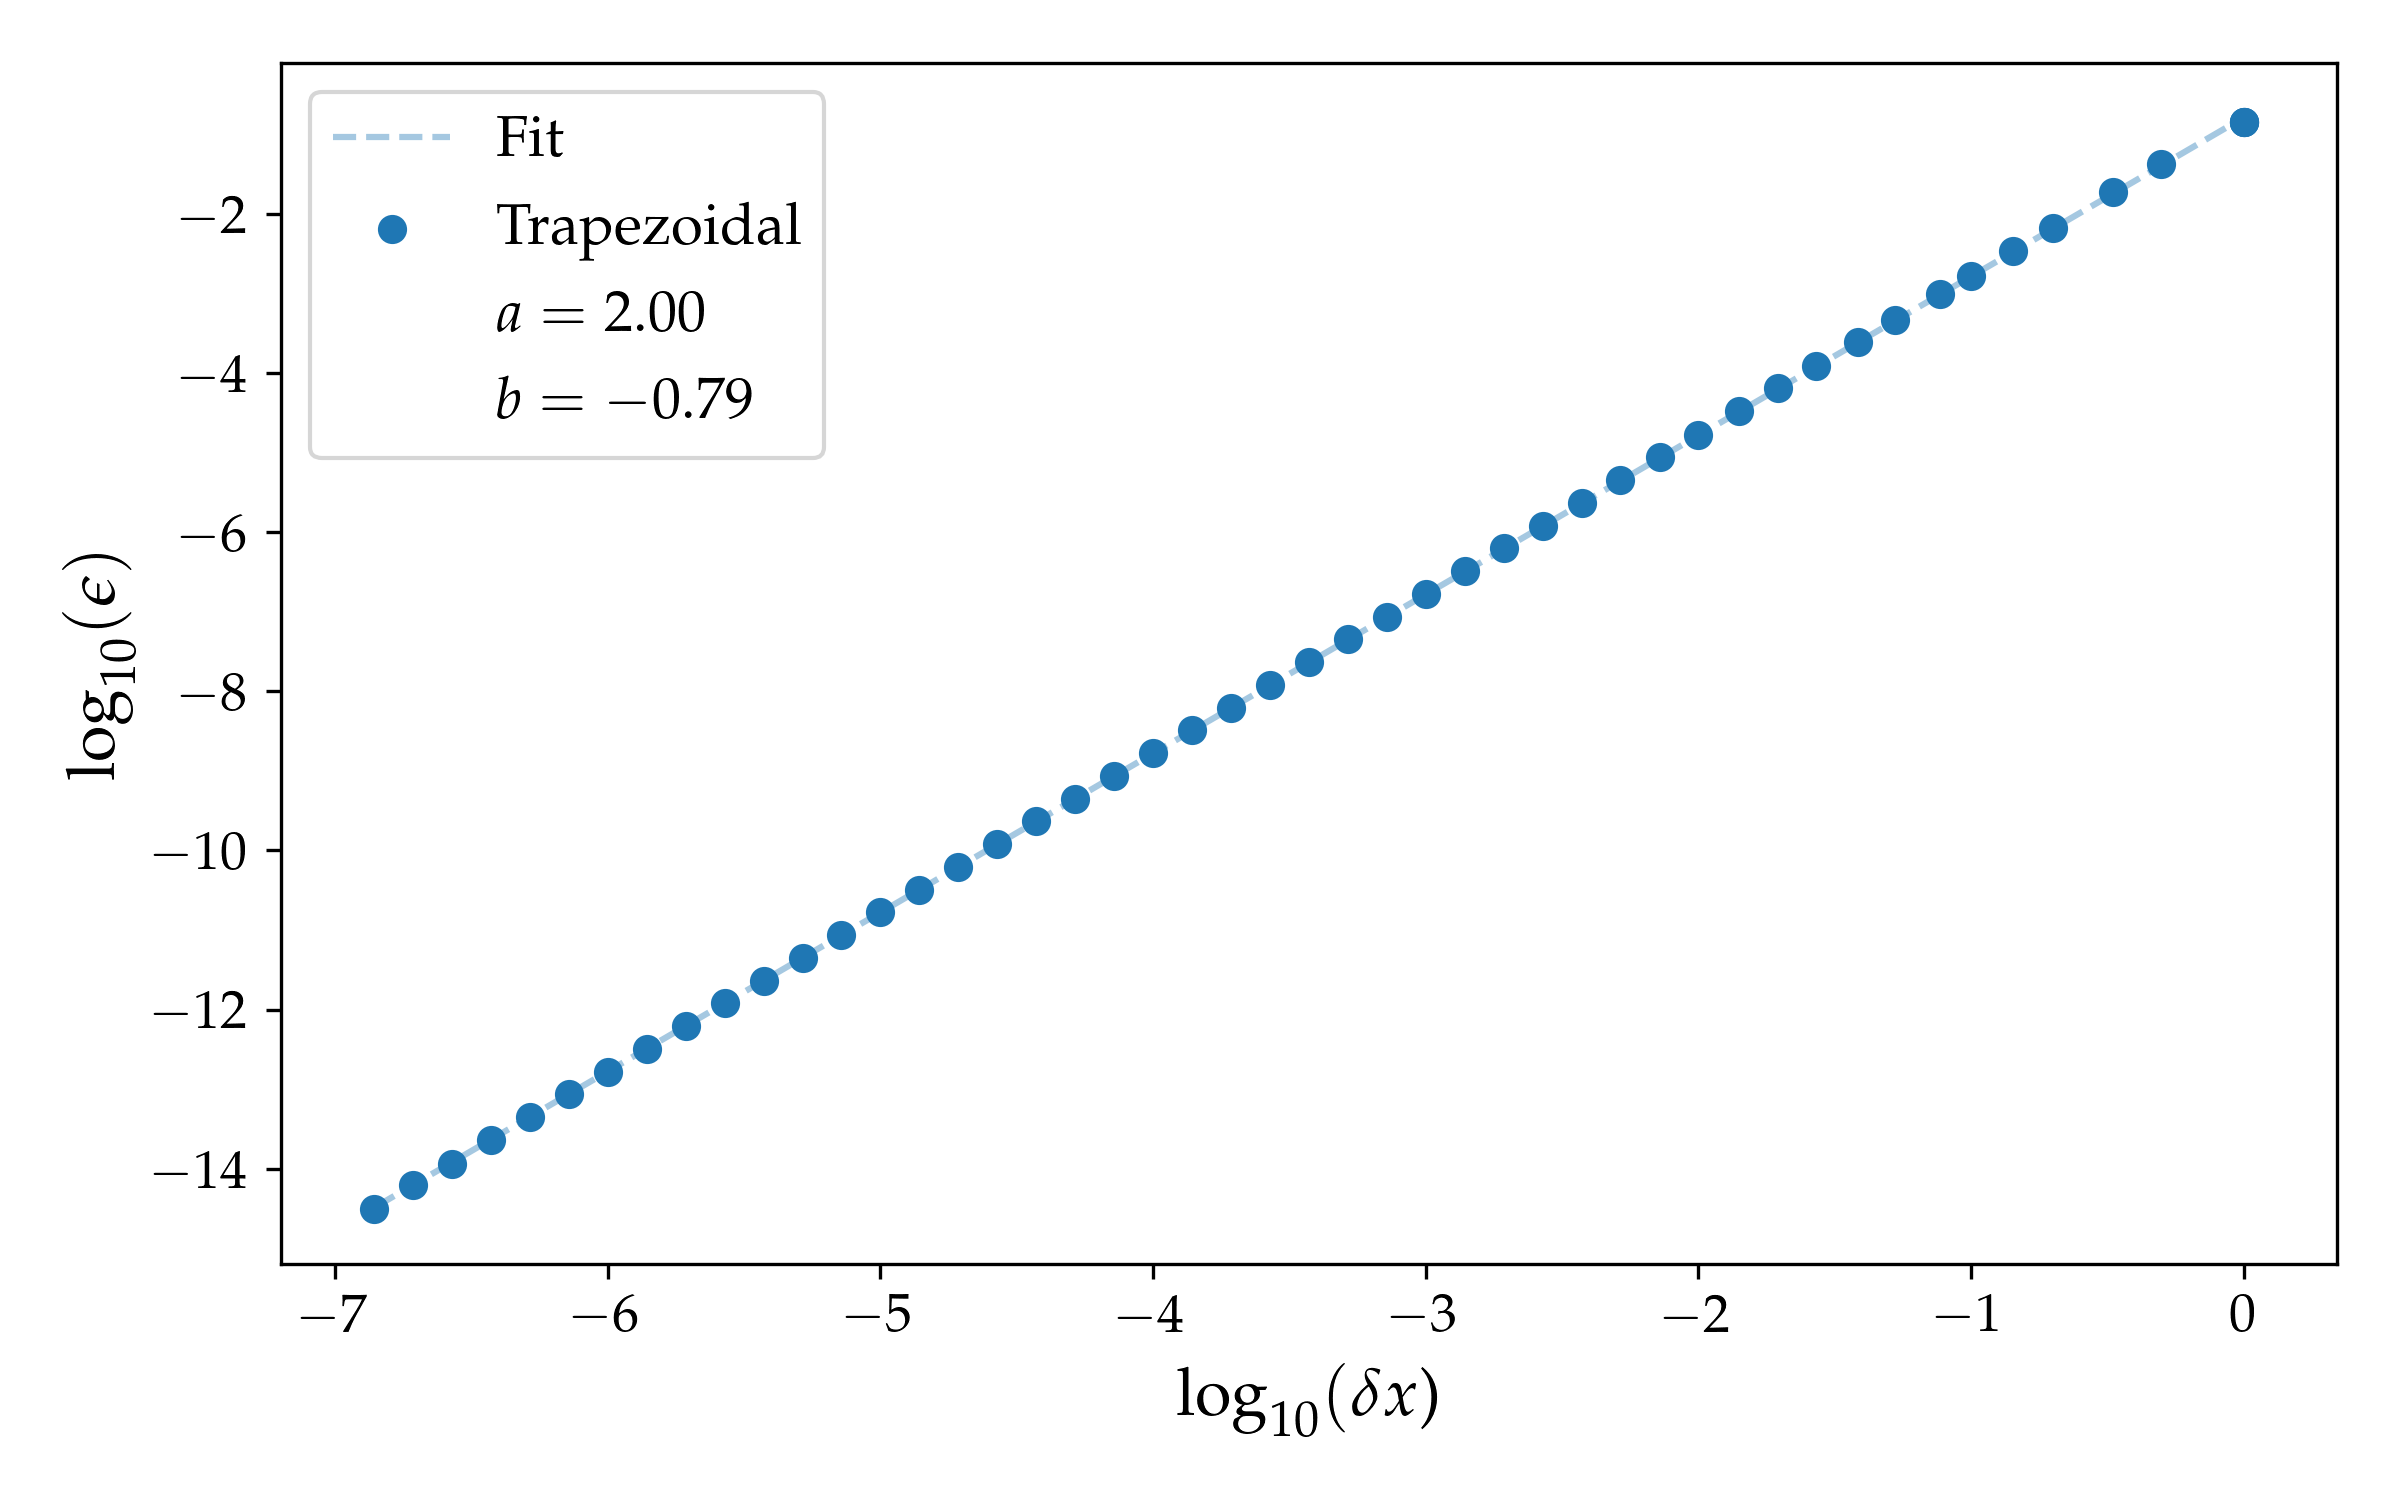
\includegraphics[width=0.8\linewidth]{images/21/FitTrap_2.png}
    \caption{Fit della convergenza del metodo dei trapezi nel caso di questo esercizio.}
    \label{fig: fit_trap_6}
\end{figure}

\begin{figure}[H]
    \centering
    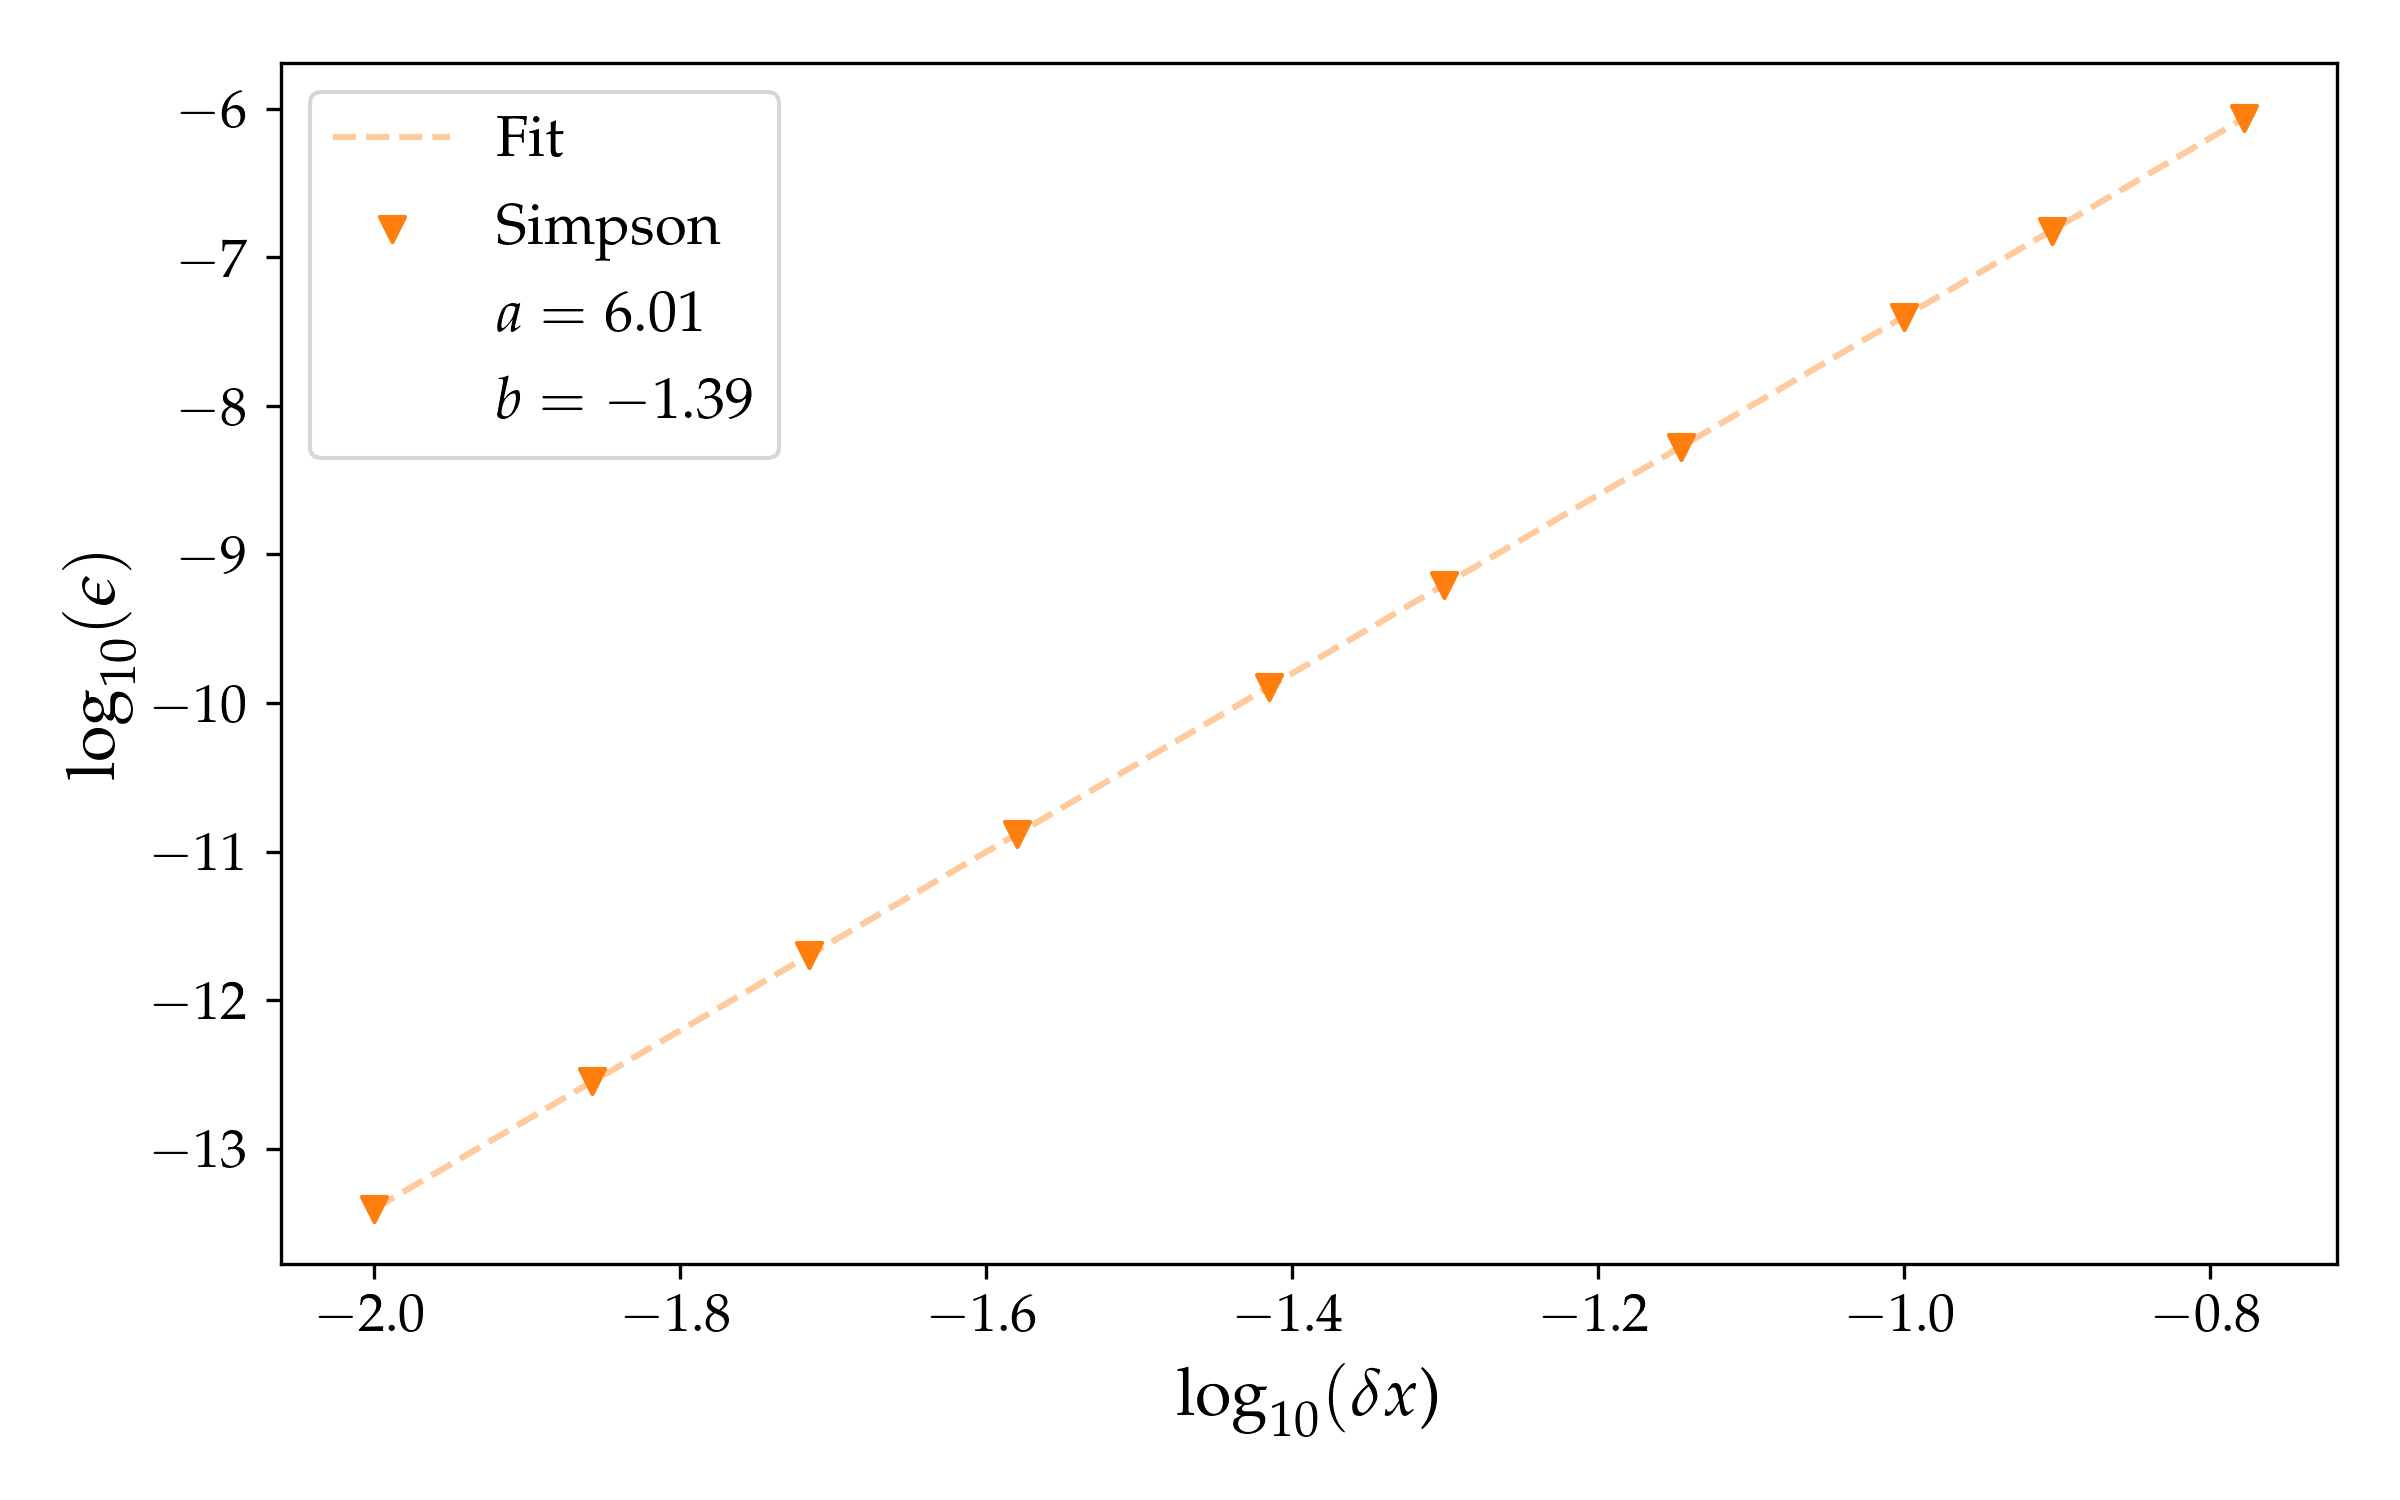
\includegraphics[width=0.8\linewidth]{images/21/FitSimp_2.png}
    \caption{Fit della convergenza del metodo di Simpson nel caso di questo esercizio.}
    \label{fig: fit_simp_6}
\end{figure}

\begin{figure}[H]
    \centering
    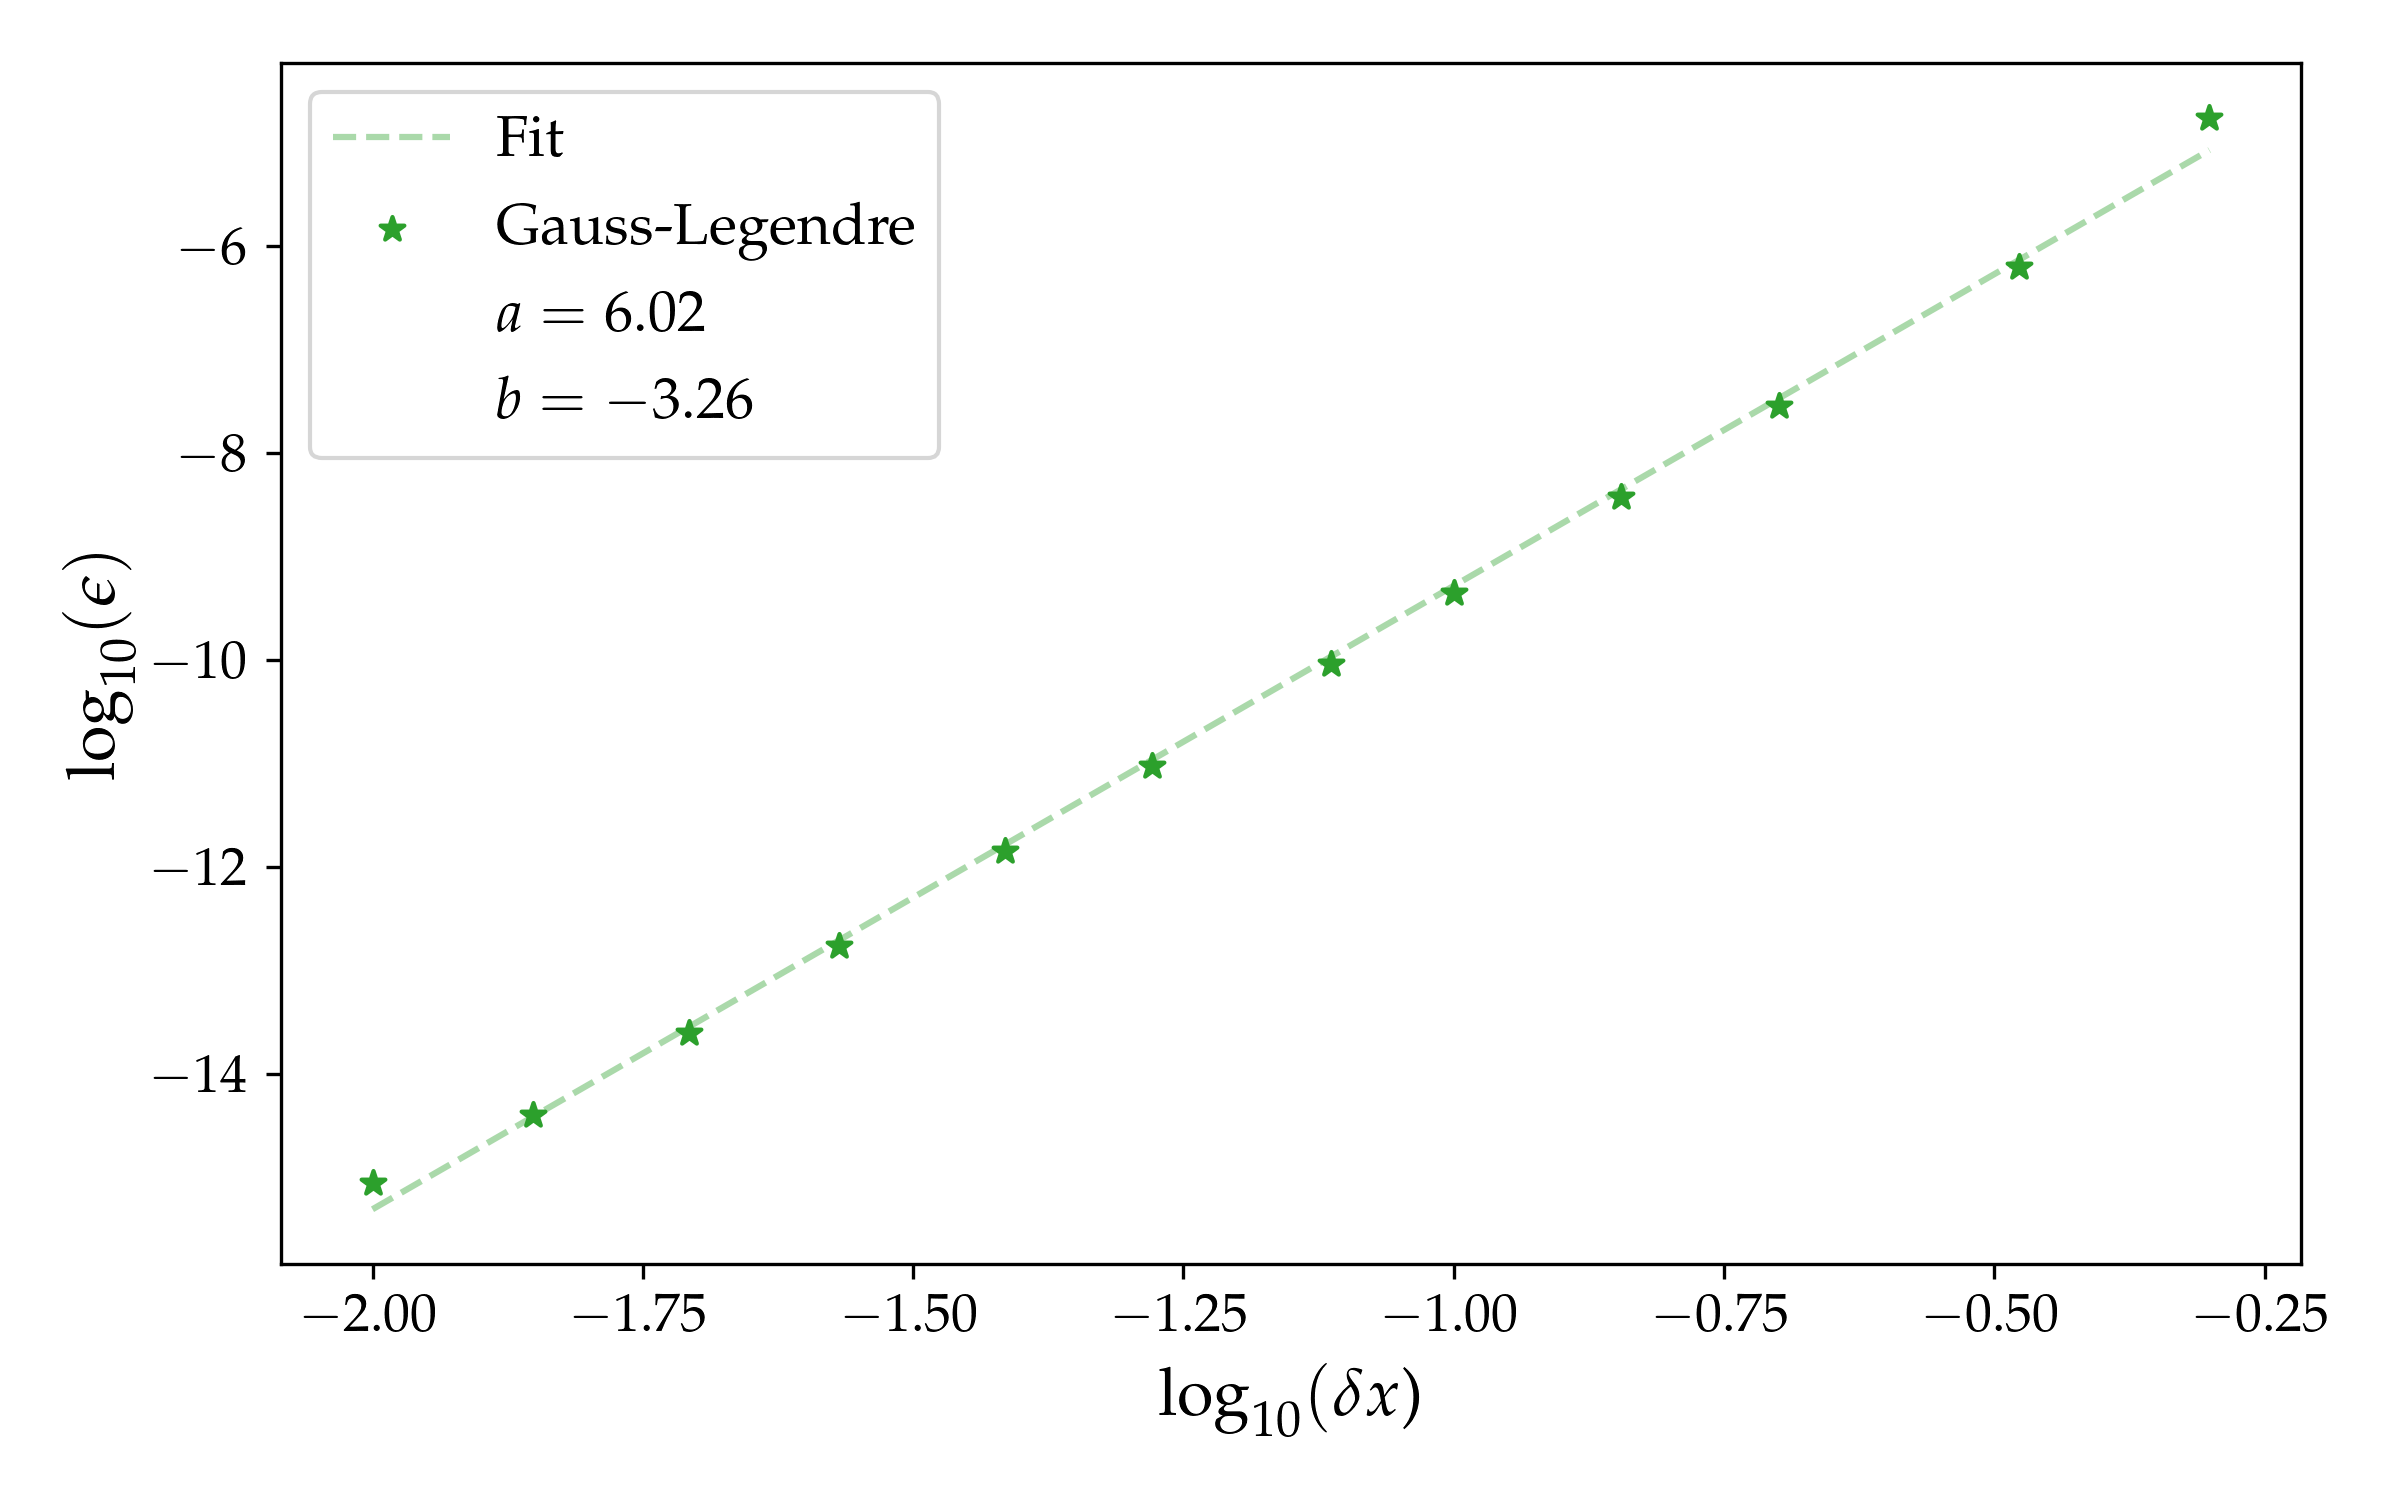
\includegraphics[width=0.8\linewidth]{images/21/FitGauss_2.png}
    \caption{Fit della convergenza del metodo della quadratura 2-punti di Gauss-Legendre nel caso di questo esercizio.}
    \label{fig: fit_Gauss_leg}
\end{figure}

\noindent L'ordine asintotico generale dei metodi rimane $p=4$; per questa particolare funzione il termine dominante dell'errore si annulla ($f^{(3)}(1) - f^{(3)}(0) = 0$), facendo emergere il termine successivo e producendo una convergenza osservata di ordine 6.\\
In maniera del tutto simile a quella dell'esercizio precedente è possibile ricavare analiticamente questo risultato, ma in questa sezione viene omesso per analogia con il sopracitato;\\
si può verificare che $f^{(5)}(b)-f^{(5)}(a)=60$, cioè che il primo termine non nullo sia quello di grado sei (le potenze dispari si annullano, a cui sono associate derivate pari).

\bigskip\noindent Possiamo quindi procedere a ricavare una stima per il numero $N$ di intervalli necessari per ottenere una determinata precisione. Se guardiamo il \textit{leading order} vale che:
$$\epsilon_G(\delta x) = O(\delta x^p) \approx k\ {\delta x}^p \Delta f^{(p-1)}$$
$$k\in \mathbb{R},\ \delta x = \frac{|b-a|}{nN}=\frac{1}{nN}, \ \Delta f ^{(p-1)} = |f^{(p-1)}(b) - f^{(p-1)}(a)|$$

\noindent Dove $n$ è un parametro proprio del metodo, per esempio $n=1$ implica che $\delta x$ sia la larghezza dell'intervallo che otteniamo dividendo in $N$ sottointervalli $b-a$, $n=2$ implica che equivalga al doppio di questa lunghezza, così procedendo.\\
Imponiamo che sia $\epsilon_G\le\varepsilon_{tol}=10^{-6}$.

\begin{align*}
    \epsilon_G &= \frac{k\ \Delta f^{(p-1)}}{n^p N^p}\le \varepsilon_{tol}\\
    \\
    N &\ge \frac{1}{n}\left(\frac{k}{\varepsilon_{tol}}\Delta f ^{p-1}\right)^{1/p}
\end{align*}

\newpage
\begin{itemize}
    \item \textbf{Trapezi}: $n=1$
    $$\epsilon_G \approx \frac{1}{12} \frac{1}{ N^2}\Delta f' = O(N^{-2})  \implies k=\frac{1}{12},\ p=2$$
    
    \item \textbf{Simpson}: $n=2$
    $$\epsilon_G \approx \frac{1}{3780} \frac{1}{N^6}\Delta f^{(5)} = O(N^{-6})  \implies k=\frac{1}{3780},\ p=6$$
 
    \item \textbf{Gauss-Legendre}: $n=1$ 
    $$\epsilon_G \approx \frac{1}{435456} \frac{1}{N^6} \Delta f^{(5)} = O(N^{-6})  \implies k=\frac{1}{435456},\ p=6$$
    
    
\end{itemize}



\bigskip\noindent

Di seguito un riassunto che ricapitola tutti i risultati raccolti
\begin{elegantcode}
Expected = 2
    p_t = 1.9970176429343596

Expected = 4
    p_s = 6.0067049348684565
    p_g = 6.0223475927006165

------------------ check ------------------

d3f(1) - d3f(0) = (-0.0) - (-0.0) = 0.0
d5f(1) - d5f(0) = (60.0) - (0.0) = 60.0

-------------------------------------------

- if Trapezoidal, p = 2, n = 1, k = 1/12:
     N = 409

- if Simpson, p = 6, n = 2, k = 1/3780:
     N = 4

- if Gauss-Legendre, p = 6, n = 1, k = 1/435456:
     N = 3
\end{elegantcode}


\bigskip\noindent Ciò che confermiamo è la gerarchia nella convergenza al valore vero dei diversi metodi, cioè possiamo mostrare come il trapezio viaggi a ordini di distanza rispetto agli altri due metodi, come velocità e costo computazionale, ma inoltre tra i due simili (entrambi quartici nella formulazione generale) la quadratura di Gauss-Legendre a 2 punti raggiunge la precisione richiesta con un numero inferiore di sottointervalli rispetto agli altri metodi, grazie anche al coefficiente numerico del termine dominante dell'errore.\\
Il grafico che segue, in Fig. \ref{fig: confr_Ndep}, rappresenta chiaramente proprio questo fenomeno, conferma le nostre ipotesi analitiche e le valutazioni fatte fino a questo momento: possiamo osservare che la \textit{treshold} fissata a $10^{-6}$ dell'errore è raggiunta dai metodi in corrispondenza delle soglie che abbiamo fissato con i nostri risultati. 

\begin{figure}[H]
    \centering
    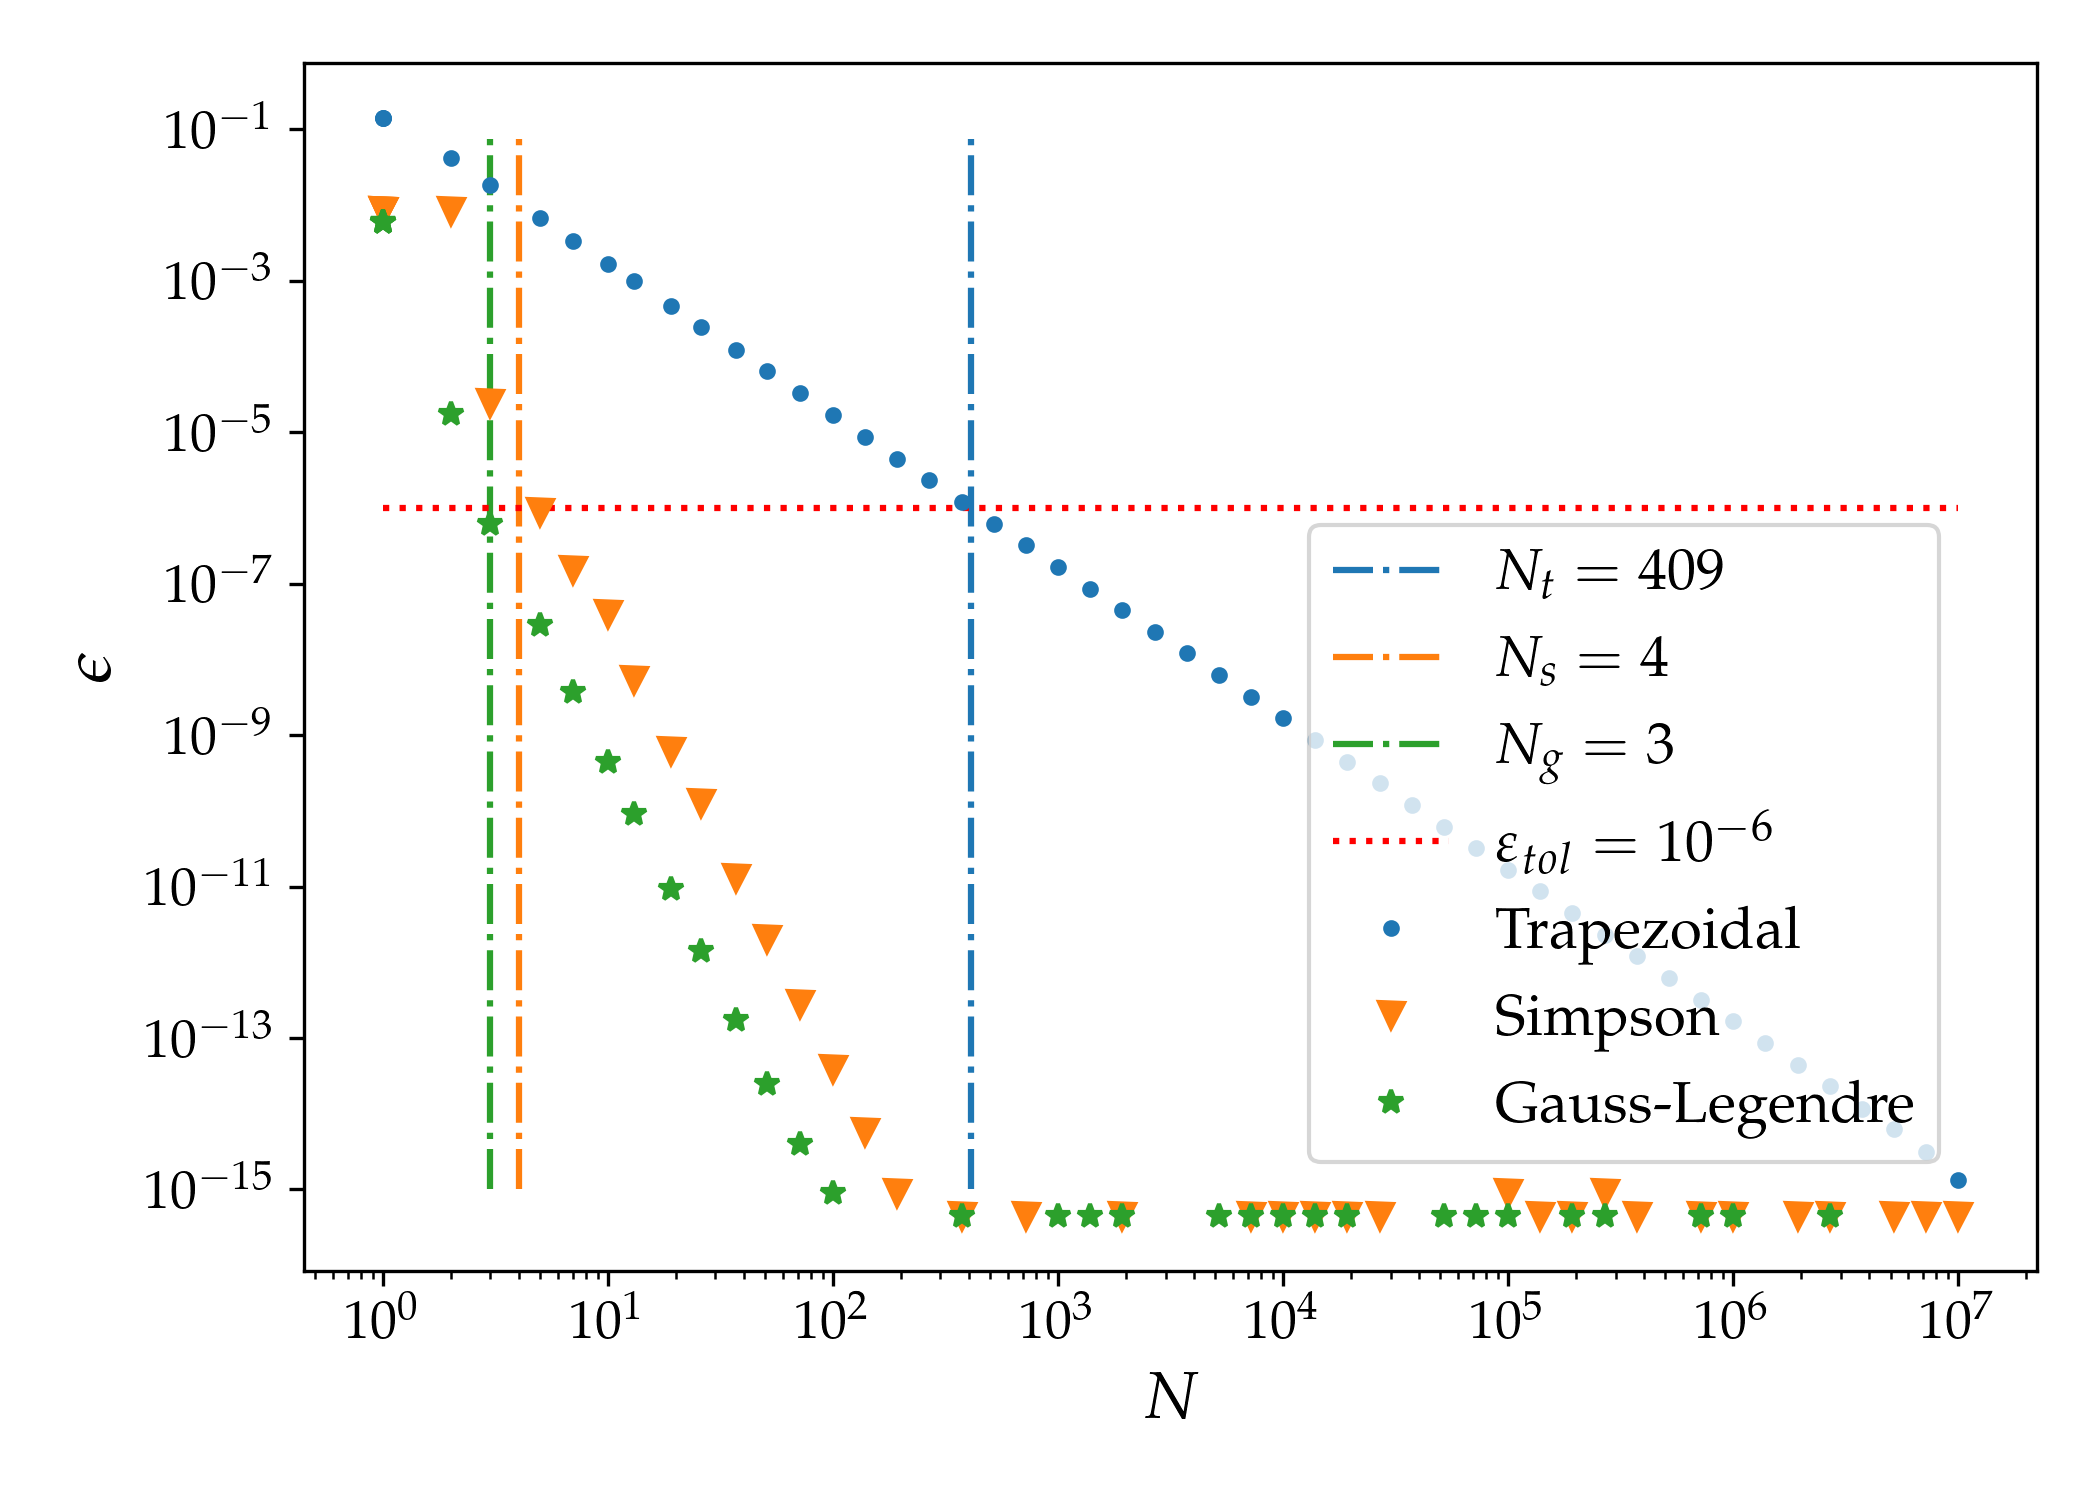
\includegraphics[width=0.8\linewidth]{images/21/check_prev.png}
    \caption{Confronto della convergenza tra i diversi metodi, in funzione di $N$, numero di intervalli in cui suddividiamo $I = [0,1]$.}
    \label{fig: confr_Ndep}
\end{figure}

\noindent L'ulteriore verifica che propongo passa attraverso il calcolo numerico dell'errore ($\epsilon =|I_{true} - I_{mth}|$) in funzione del numero di intervalli determinato: si confronti con il valore di riferimento di $\varepsilon_{tol}=10^{-6}$

\begin{elegantcode}
TRAPEZOIDAL:
   e = 9.96e-07

SIMPSON:
   e = 1.51e-07

GAUSS-LEGENDRE:
   e = 6.21e-07

\end{elegantcode}

\newpage











\section{Esercizio 8.2.2}
\subsection{Problem Statement}
Per i polinomi di Hermite $H_n$, la condizione di ortogonalità è

$$(H_n, H_m) = \sqrt{\pi} 2^n n! \delta_{nm}$$


Essi soddisfano la relazione


$$H_{n+1}(x) = 2xH_n(x) - 2nH_{n-1}(x), \quad H_0(x) = 1, \quad H_{-1}(x) = 0$$


Scrivere un programma che, data una funzione $f(x)$ e un numero intero $n$, esegua i seguenti compiti:
\begin{enumerate}
\item Calcolare le radici del polinomio di Hermite di ordine $n$, $H_n(x)$; per questo compito, riutilizzare il programma già scritto nella sezione relativa alle radici delle funzioni.
\item Calcolare i pesi di Gauss-Hermite $w_i$ utilizzando


$$w_i = \frac{2^{n-1} n! \sqrt{\pi}}{n^2 [H_{n-1}(x_i)]^2}$$


\item Approssimare l'integrale


$$\int_{-\infty}^{\infty} dx \, e^{-x^2} f(x) \approx \sum_{i=1}^{n} w_i f(x_i)$$


\end{enumerate}
Studiare i seguenti integrali con la quadratura di Gauss-Hermite e la loro convergenza per diversi valori di $n$:
\begin{enumerate}
\item $\int_{-\infty}^{\infty} dx \frac{e^{-x^2}}{1+x^2}$
\item $\int_{0}^{\infty} dx \, x^8 e^{-x^2}$
\item $\int_{3}^{\infty} dx \, x^5 e^{-x^2}$
\end{enumerate}
Tracciare un grafico dei pesi $w_i$ sull'asse $y$ e delle radici $x_i$ sull'asse $x$, per diversi valori di $n$ nel caso $(-\infty, \infty)$. Per l'ultimo integrale confrontare i risultati con uno studio (in funzione del numero di punti) usando la regola dei trapezi e di Simpson.

\subsection{Premessa Teorica}
In generale la formulazione che abbiamo definito per la quadratura 2 punti di Gauss-Legendre (facente uso delle radici dei polinomi ortogonali di Legendre) può essere generalizzata sul numero di punti e il tipo di polinomio ortogonale da usare per il metodo. Ciascuno di essi ha delle proprie caratteristiche e un dominio sul quale lavorare. Associati ai polinomi è necessario riconoscere le loro funzioni peso, specifiche per ciascuno di essi.\\
Questi metodi permettono delle ottime prestazioni, ma come si è mostrato, richiedono alcune caratteristiche specifiche e non banali.


\subsection{Metodi Numerici e Algoritmi}
Nel caso dell'esercizio precedente lavoravamo con i polinomi di Legendre che hanno funzione peso $w(x_i) =1,\  \forall x_i$, dove $x_i$ sono i nodi (radici del polinomio). Anche non riconoscendola esplicitamente essa è banalmente integrata nella definizione della funzione qualsiasi.\\
Per questo esercizio ci concentriamo sull'uso dei polinomi di Hermite, utilizzando la funzione peso
$$w_i = \frac{2^{n-1} n! \sqrt{\pi}}{n^2 [H_{n-1}(x_i)]^2}$$

La difficoltà nei casi di studio è rappresentata dalla necessità di rimappare gli integrali su degli intervalli adatti per il metodo che stiamo usando. La quadratura di Gauss-Hermite viene definita su un intervallo simmetrico di $(-\infty, +\infty)$ e necessita di riconoscere esplicitamente il peso $e^{-x^2}$: dobbiamo quindi passare, attraverso un cambio di variabili o una riscrittura, da:
\[
\int_{a}^{b} dx\ f(x) \quad \longrightarrow \quad \int_{-\infty}^{+\infty} dt\ g(t) e^{-t^2} \approx \sum_{i=1}^n w_i g(x_i)
\]



\subsection{Risultati e Discussione}
\begin{enumerate}
    \item $\int_{-\infty}^\infty dx \frac{e^{-x^2}}{1+x^2} = \pi e\ \text{Erfc(1)}\approx1.34$
    
    \medskip\noindent
    Questo primo caso è già esplicitato nella forma necessaria: in particolare $f(x) = \frac{1}{1+x^2}$.
    Si possono illustrare qui di seguito i risultati ottenuti; in questo tipo di rappresentazioni (dell'output del programma) trattandosi di un caso di test di cui è nota la soluzione analitica, ai fini della nostra analisi assumiamo come miglior stima il valore dell'iterazione che minimizza lo scarto con il valore vero. In un'applicazione priva di soluzione nota, l'instabilità della convergenza (che non risulta monotona decrescente) renderebbe necessario un criterio di arresto basato sulla minima differenza tra approssimazioni successive, prima dell'insorgere del rumore numerico.

\begin{elegantcode}
Results of the study:
     TRUE                --> I = 1.3432934216467347

     Gauss quadrature    --> I = 1.3434104959189055
                             err = 1.17e-04
\end{elegantcode}

    In particolare la Fig. \ref{fig: int_1} esplicita quale sia il comportamento che caratterizza l'algoritmo nel corso delle iterazioni. Si osserva che la convergenza non è stabile, ha invece un salto brusco raggiunto un certo numero di nodi (nello specifico caso $n\gtrsim 17$ peggiora l'errore, per $n\gtrsim 21$ gli errori di overflow bloccano l'esecuzione): la perdita di accuratezza osservata è dovuta all'implementazione numerica adottata per il calcolo dei polinomi e dei pesi, che porta a overflow e cancellazioni numeriche per ordini elevati, non a una limitazione intrinseca della quadratura di Gauss-Hermite. Si noti come
    \[
    w_i(n) \propto \frac{(n-1)!}{n} 
    \]
    In Fig. \ref{fig: asymp_wei} la rappresentazione di questo andamento asintotico, dove si può notare come, fissata una tolleranza numerica a $\varepsilon_{tol}=10^{-16}$ (indicativa del numero di cifre significative in \textit{double precision}), si trova circa in corrispondenza del valore a cui facevamo riferimento prima, che raggiungiamo dei valori della funzione peso $w_i\approx1/ \varepsilon_{tol}$. 
    
    Aumentando il numero di nodi oltre $n=21$ si verifica numericamente che non è possibile procedere con il calcolo, poiché si rilevano errori di overflow. 

    
    \begin{figure}[H]
        \centering
        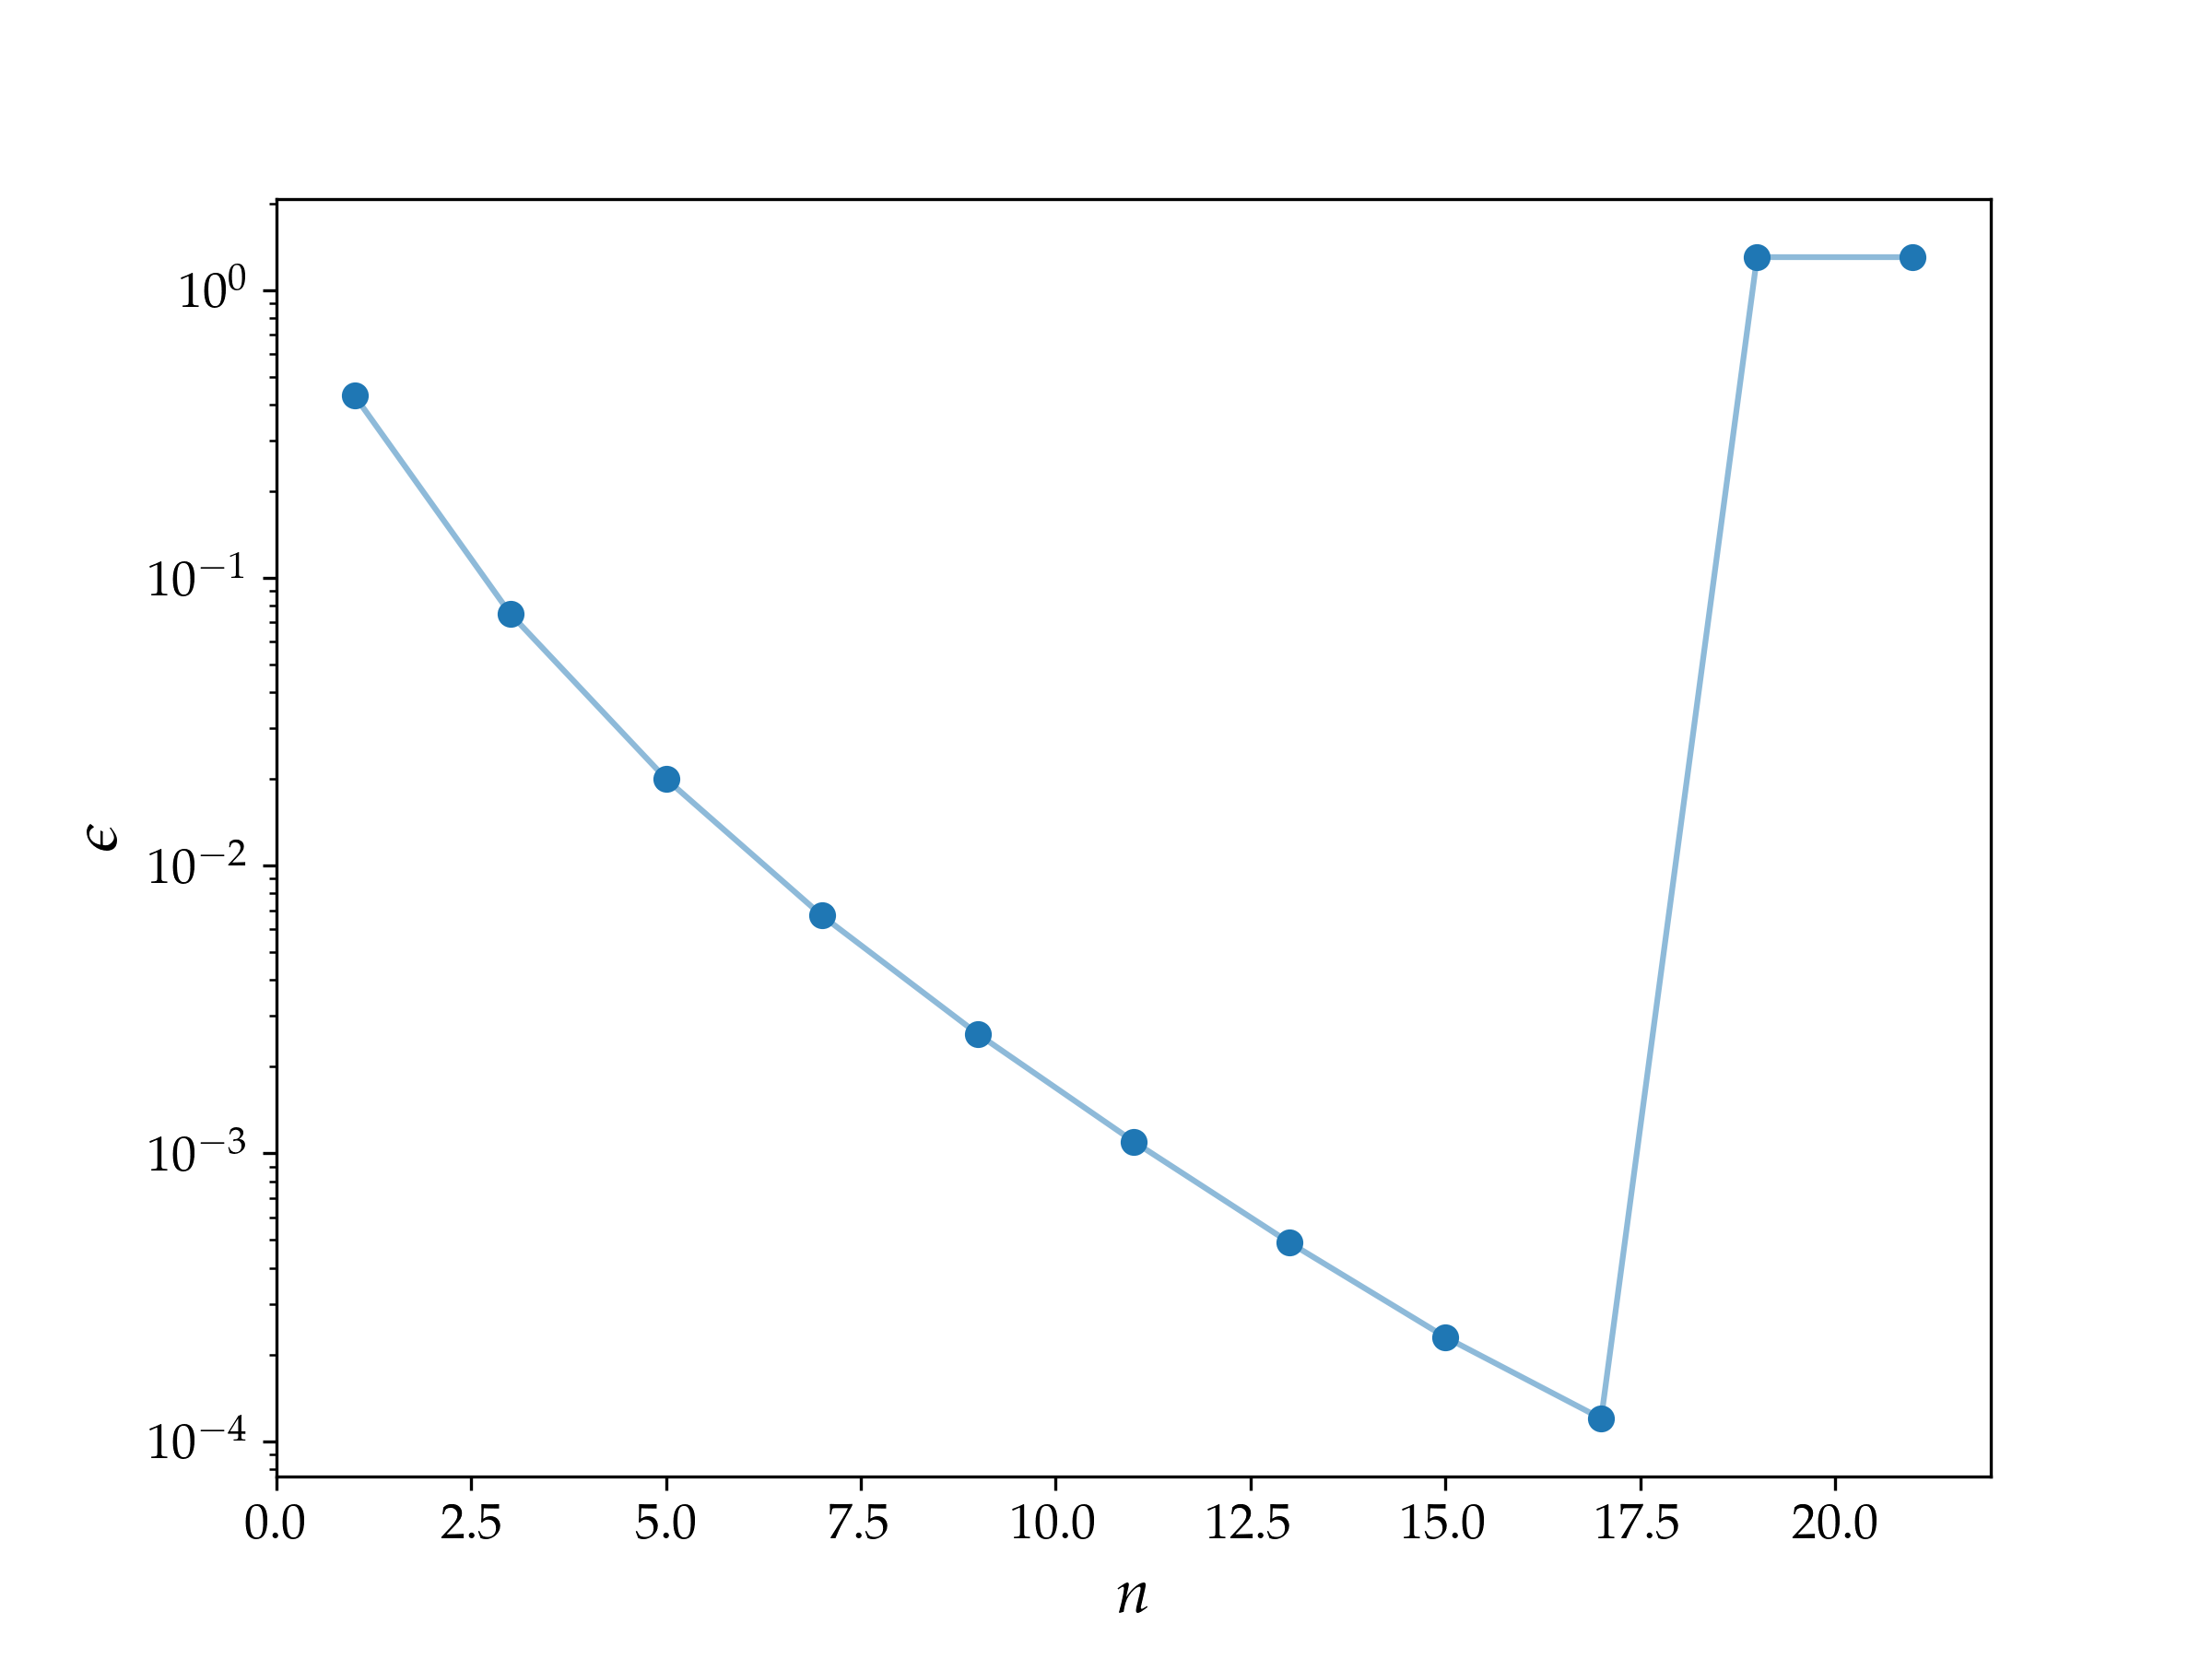
\includegraphics[width=0.7\linewidth]{images/22/int_1.png}
        \caption{Andamento dell'errore per l'integrale $I_1$, in funzione del numero di nodi (radici del polinomio di Hermite).}
        \label{fig: int_1}
    \end{figure}

    \begin{figure}[H]
        \centering
        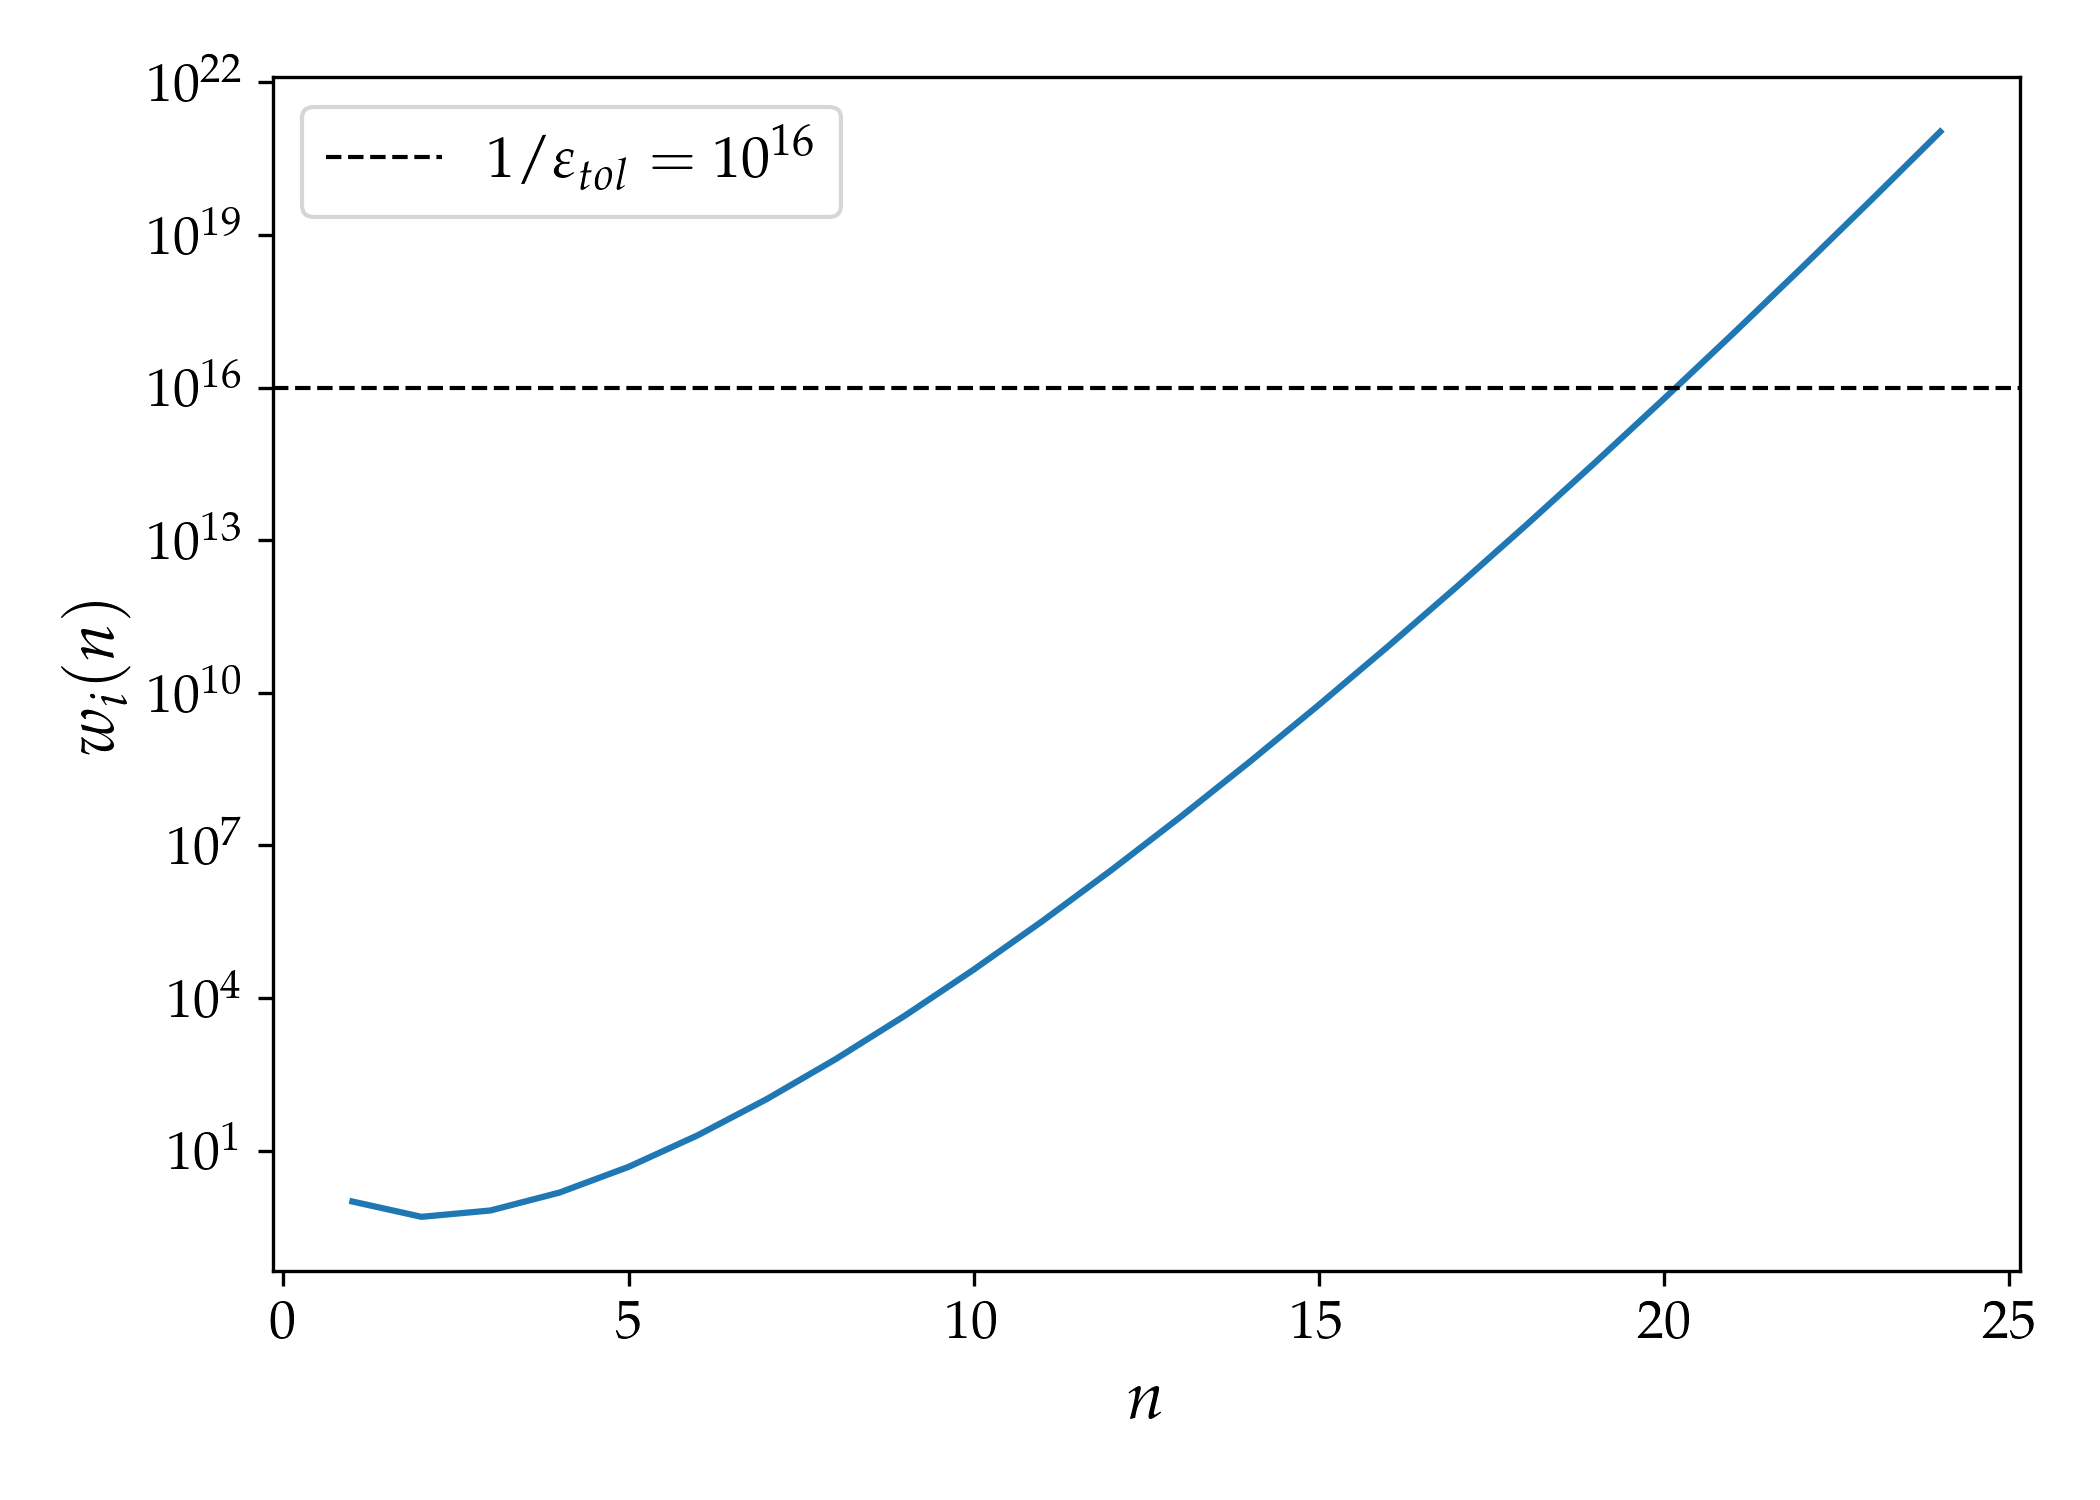
\includegraphics[width=0.7\linewidth]{images/22/asym_weight.png}
        \caption{Andamento asintotico della funzione $w_i$ in funzione di $n$. Nel grafico viene rappresentata $f(n) = \frac{(n-1)!}{n}$}
        \label{fig: asymp_wei}
    \end{figure}

    
    
    
    
    \item $\int_0^\infty dx \, x^{8} \, e^{-x^2} = \frac{105}{32}\sqrt{\pi}\approx 5.82$
    
    \medskip\noindent
    Il caso della seconda funzione ha la caratteristica di non trovarsi in forma esplicita così come ci viene presentata: dobbiamo riportare l'integrale con le condizioni necessarie per l'applicazione del metodo.

    In particolare sapendo che la funzione $h(x) = x^8e^{-x^2}$ è pari, possiamo ridefinire semplicemente sull'intervallo simmetrico come:
    \[
    \int_0^\infty dx \, x^{8} \, e^{-x^2} \to \int_{-\infty}^\infty dx \, \frac{x^{8}}{2} \, e^{-x^2}
    \]

    La funzione $f(x)$ per l'algoritmo diventa quindi:
    \[
    f(x) = \frac{x^{8}}{2} 
    \]

    I risultati numerici di seguito, in Fig. \ref{fig: int_2} lo studio in funzione di $n$.

\begin{elegantcode}
Results of the study:
     TRUE                --> I = 5.815864198283724

     Gauss quadrature    --> I = 5.8158641982835775
                             err = 1.47e-13
\end{elegantcode}

    In particolare si noti come l'errore raggiunga un minimo per un piccolo numero di nodi ($n=7$), poi inizia a crescere per infine attestarsi su un plateau, non convergendo definitivamente a valore vero. La spiegazione è del tutto simile a quella fatta per il caso precedente.  
    
    \begin{figure}[H]
        \centering
        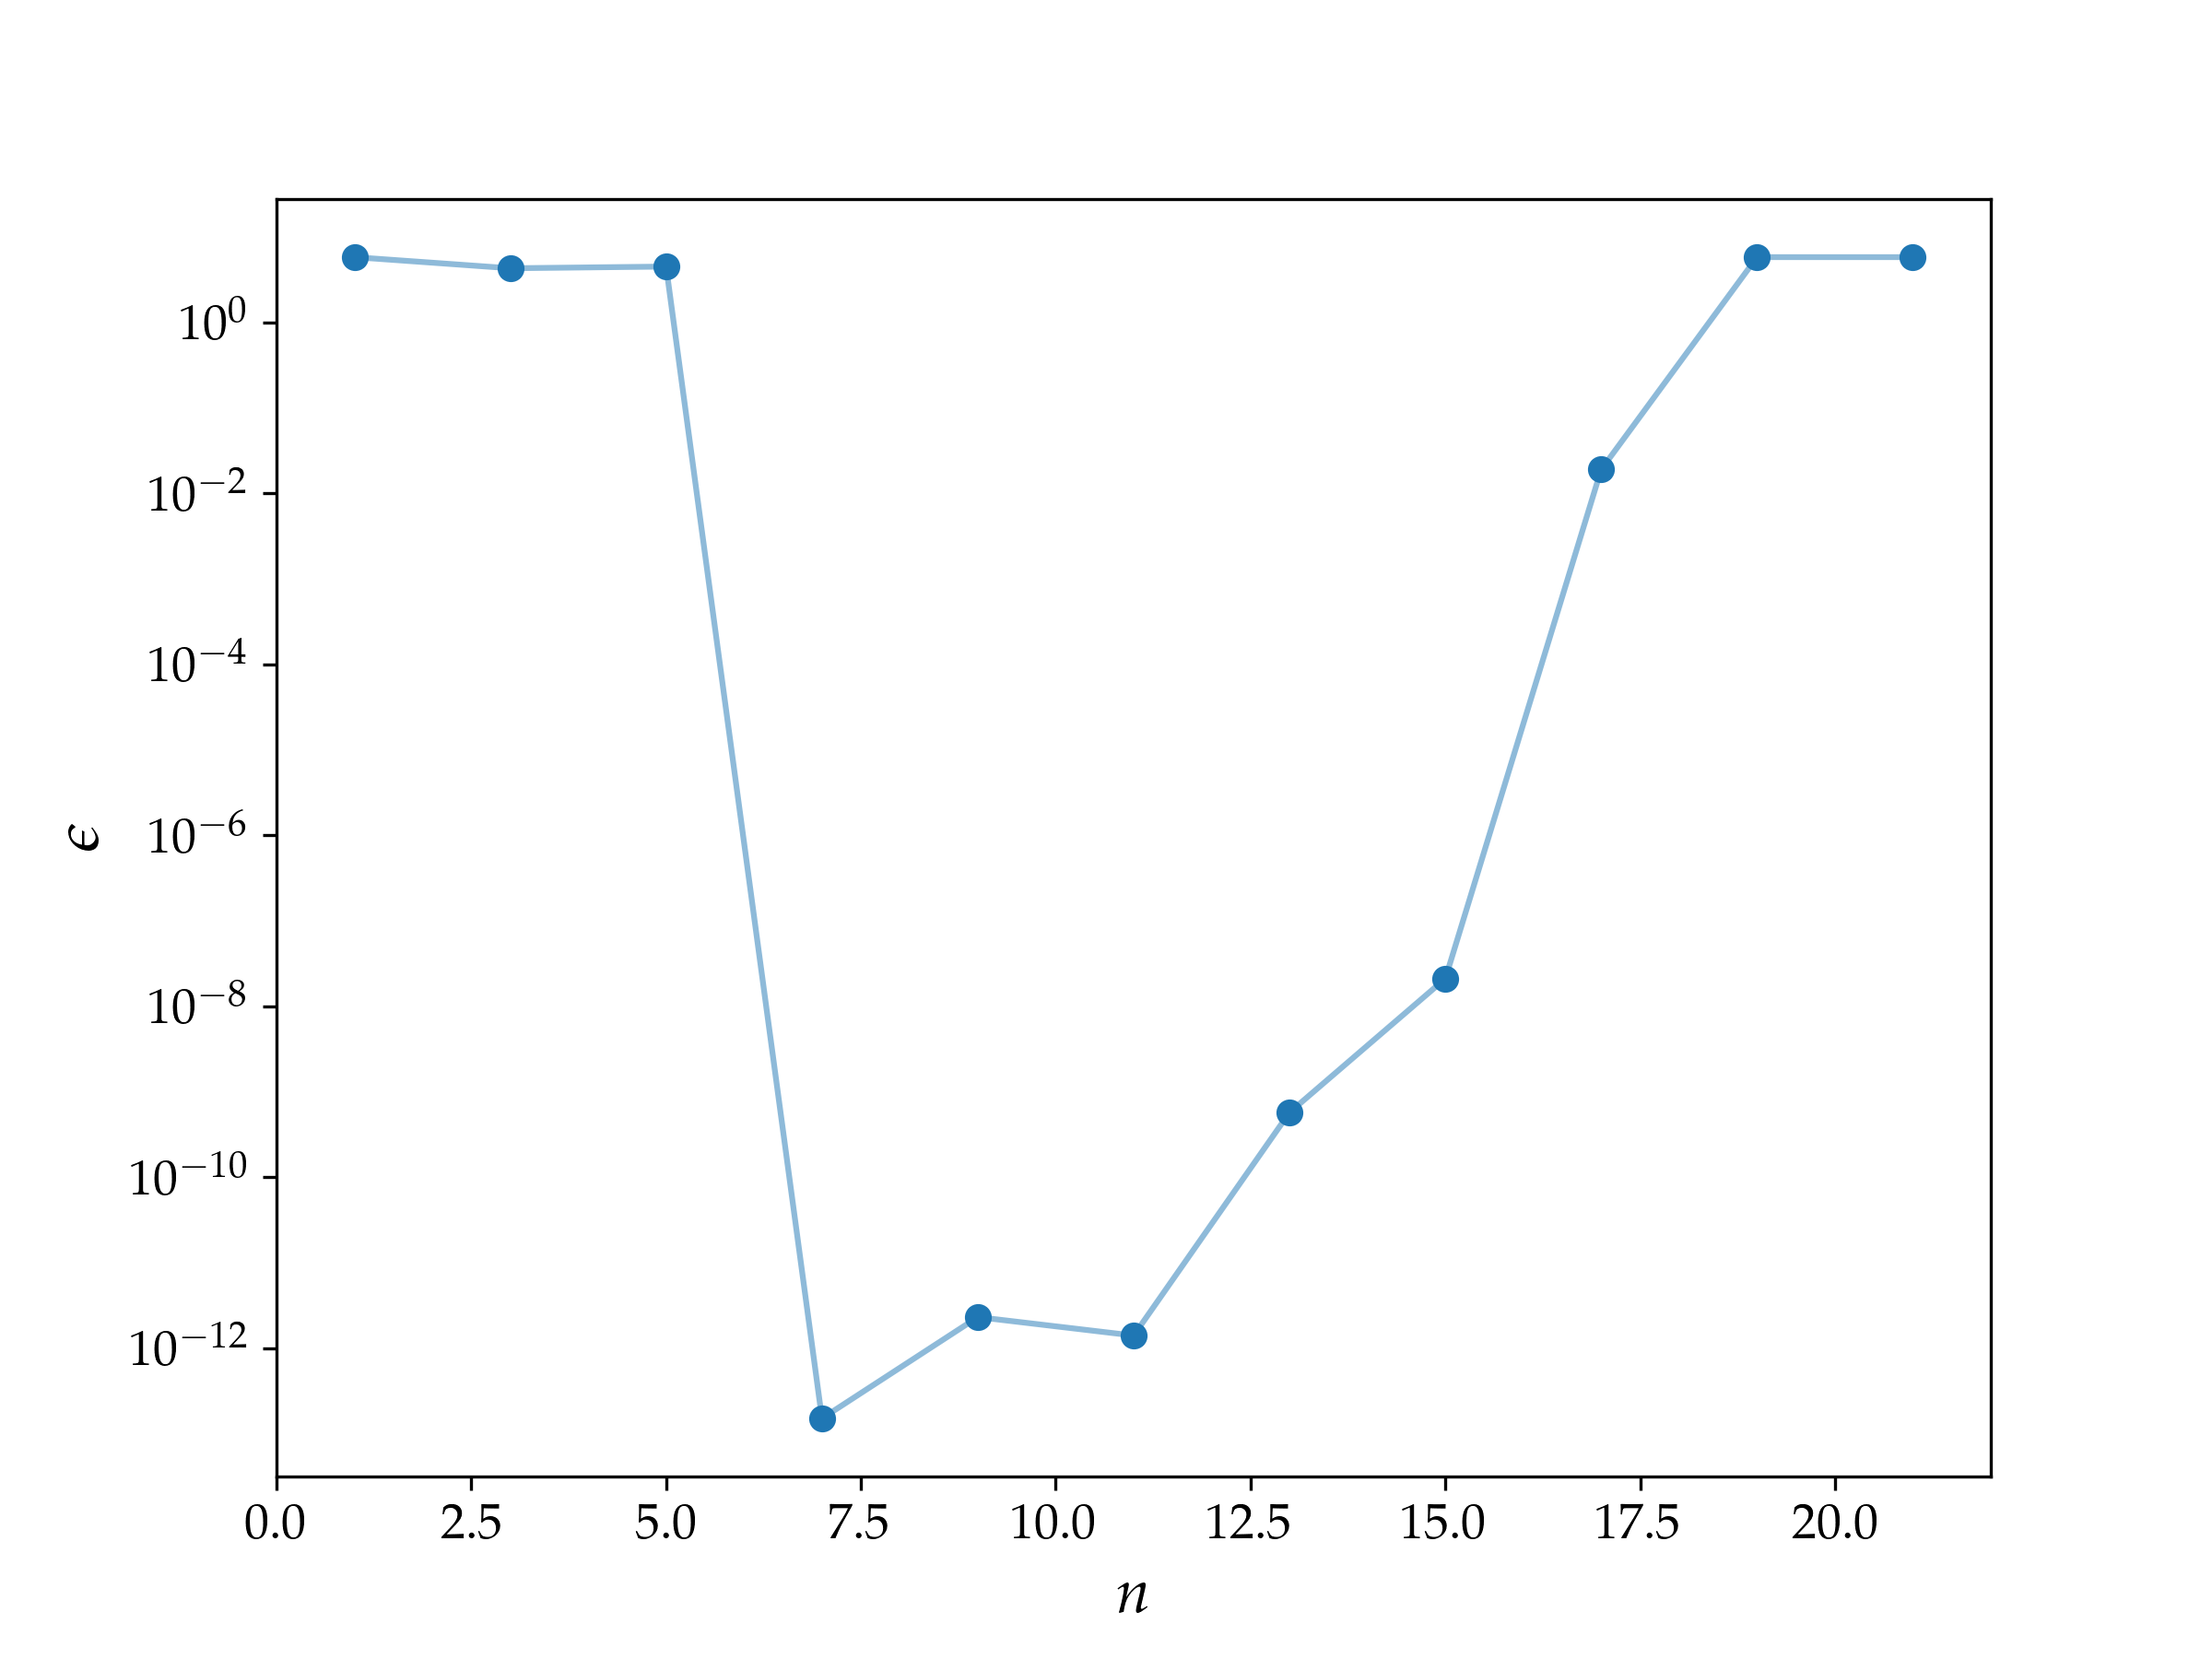
\includegraphics[width=0.7\linewidth]{images/22/int_2.png}
        \caption{Andamento dell'errore per l'integrale $I_2$, in funzione del numero di nodi (radici del polinomio di Hermite).}
        \label{fig: int_2}
    \end{figure}

    
    
    \item $\int_{3}^\infty dx x^5 \, e^{-x^2}=\frac{101}{2}e^{-9}\approx 6.23 \times10^{-3}$
    
    \medskip\noindent
    Infine per questo ultimo caso riportare la funzione nella forma analitica richiesta, non mi è stato possibile. Non ho trovato alcuna caratteristica che potesse permettere un cambio di variabili utile o una simmetrizzazione come nel secondo caso. La mia scelta è stata di definire 
    \[
    f(x) = x^5 H(x-3)
    \]

    dove $H(x-3)$ è la funzione di Heaviside, che vale:
    $H(x) = $
\begin{cases}
1   \quad x\ge3\\
0   \quad x<3
\end{cases}

    così facendo annulliamo manualmente la funzione al di fuori del nostro dominio di interesse, introducendo però una delta di dirac nella derivata (la derivata di $H'(x=3)$ in senso distribuzionale è proprio la $\delta(3)$). La funzione non è più liscia come ipotizzavamo introducendo questo metodo di risoluzione; la discontinuità degrada l'ordine pratico di convergenza e rende la quadratura molto meno efficiente. Potremo osservare come questa scelta introduce un certo grado di oscillabilità nella soluzione numerica, che non potrà competere con la precisione degli altri metodi di integrazione, come sarà possibile notare nei confronti diretti.

    Seguono i risultati dello studio, che è stato ripetuto anche per gli altri metodi numerici, associando al valore di $n$ il significato di numero di intervalli in cui viene suddiviso il $\Delta x$, cioè l'intervallo grande in cui valutiamo la funzione. Gli algoritmi che avevamo già introdotto, quello dei trapezi e di Simpson, possono lavorare direttamente con la formula analitica fornita in prima battuta, a patto di scegliere un intervallo di integrazione finito: se $I=[3, +\infty)$ è l'intervallo originario, imponiamo che i metodi lavorino su $\Tilde{I} = [3, 7]$. 
    
    Si verifica che la funzione è monotona decrescente per $x>3$ e che $f(7)\approx10^{-17}$, cioè al di sotto della nostra \textit{machine precision}. Consideriamo la funzione sulla parte destra di questo intervallo trascurabile per le nostre valutazioni. 
    In Fig. \ref{fig: val_func} si mostra l'intervallo di valutazione che abbiamo appena commentato.

\begin{elegantcode}
Results of the study:
     TRUE                --> I = 6.23e-03

     Gauss quadrature    --> I = 7.43e-03
                             err = 1.19e-03

     Trapezoidal         --> I = 6.62e-03
                             err = 3.90e-04

     Simpson             --> I = 6.24e-03
                             err = 8.82e-06
\end{elegantcode}

    
    \begin{figure}[H]
        \centering
        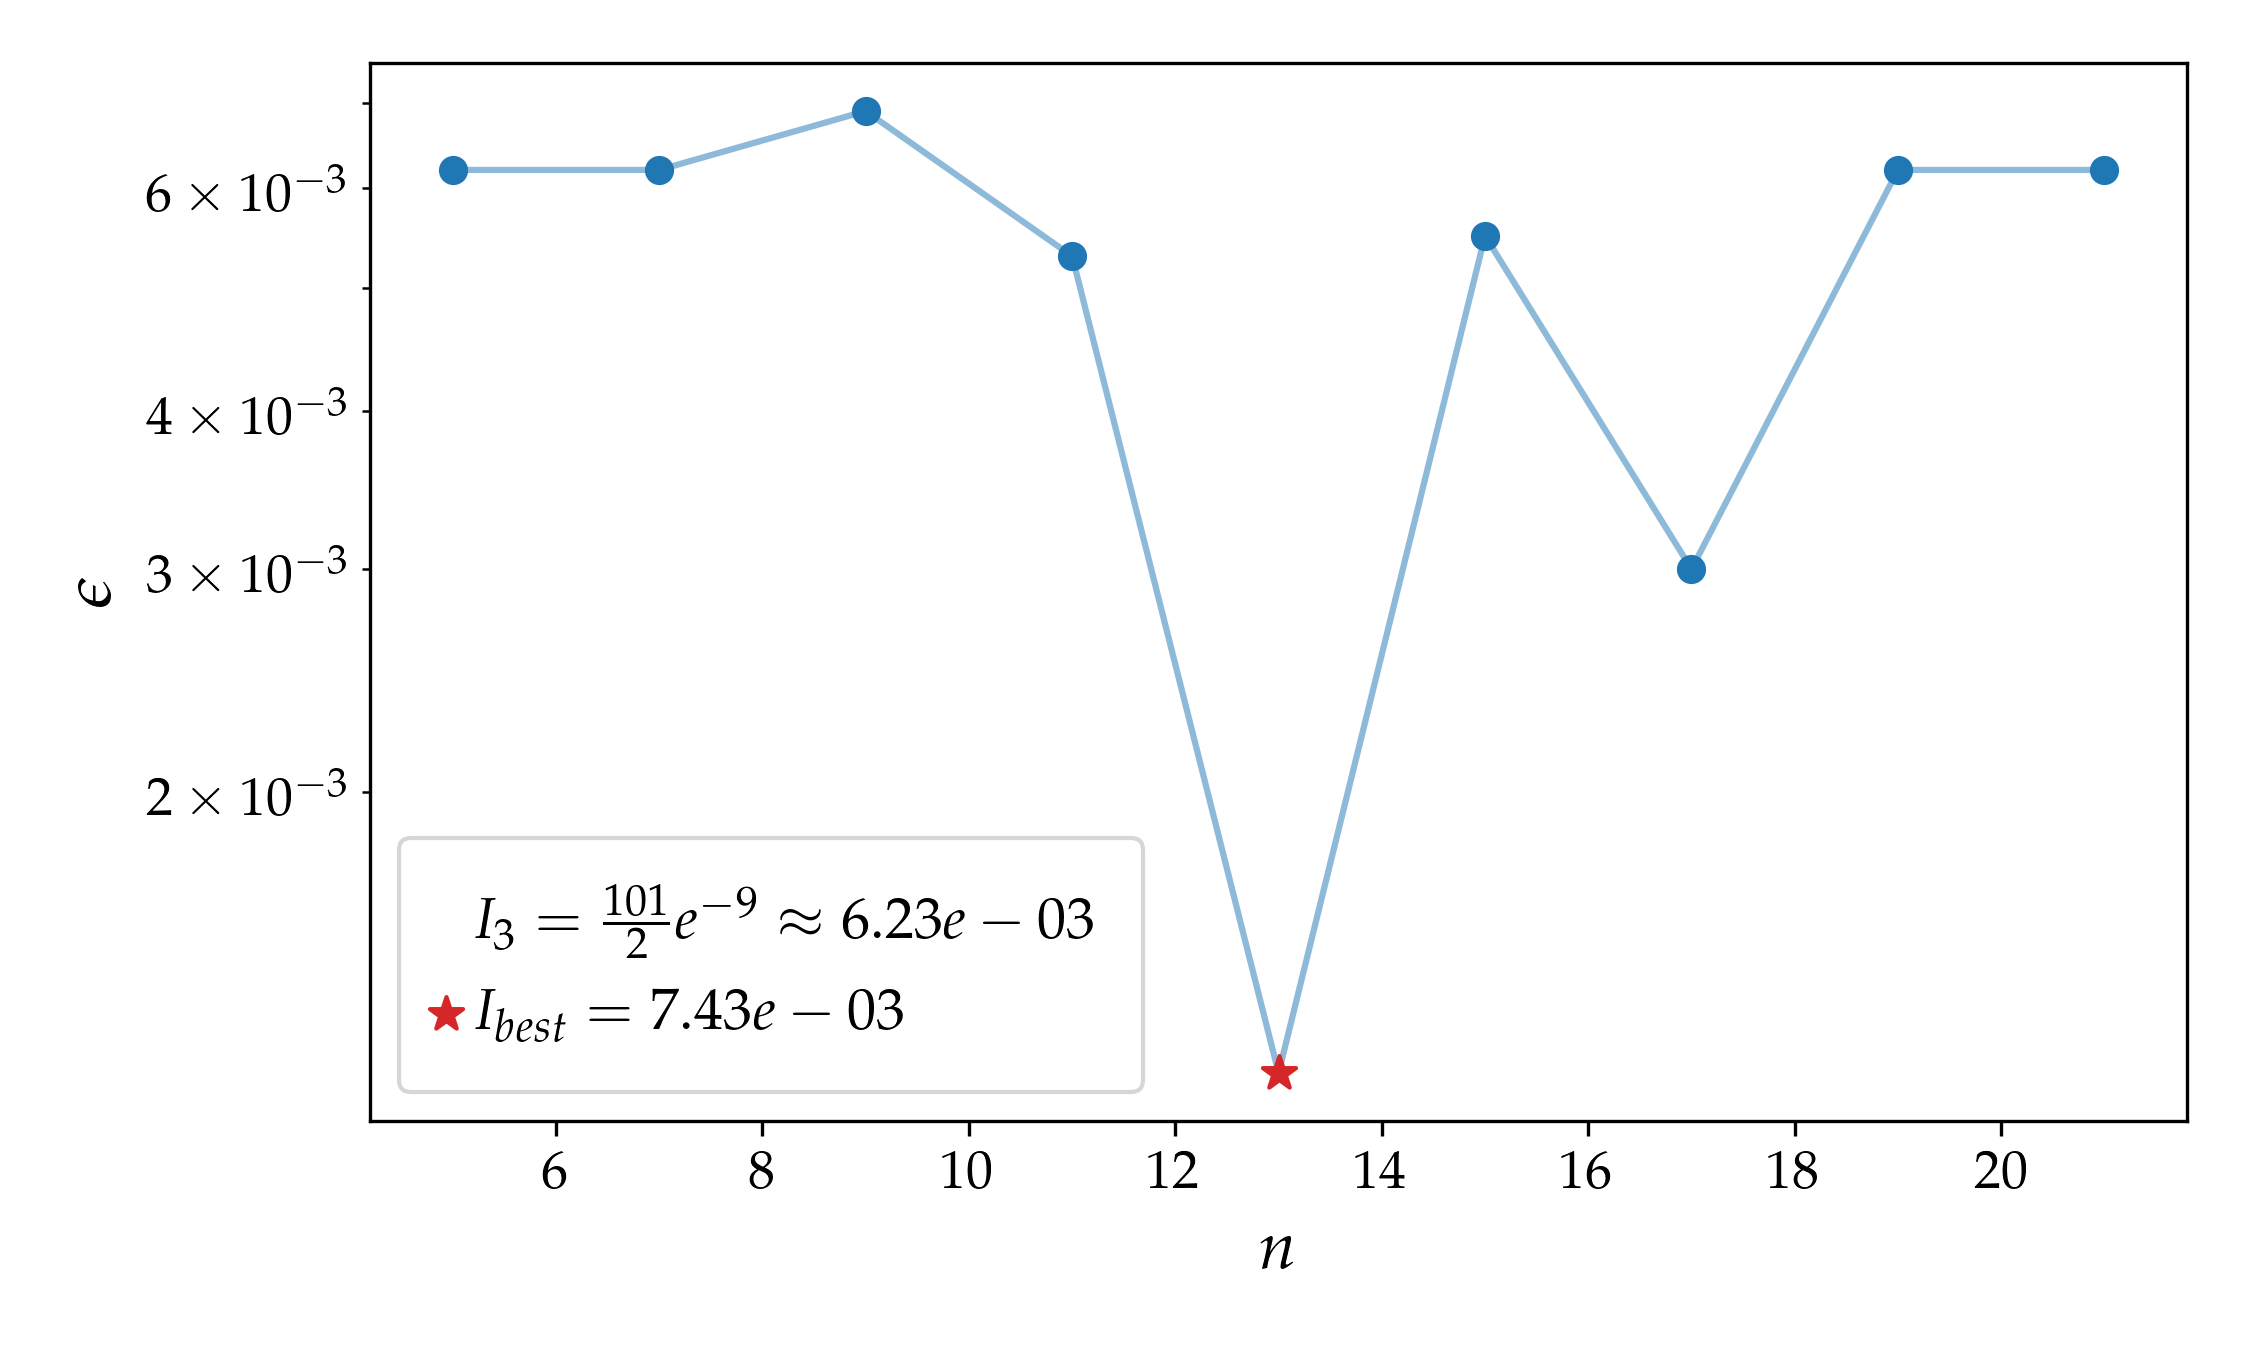
\includegraphics[width=0.7\linewidth]{images/22/int_3.png}
        \caption{Andamento dell'errore per l'integrale $I_3$, in funzione del numero di nodi (radici del polinomio di Hermite).}
        \label{fig: int_3}
    \end{figure}
    
    \begin{figure}[H]
        \centering
        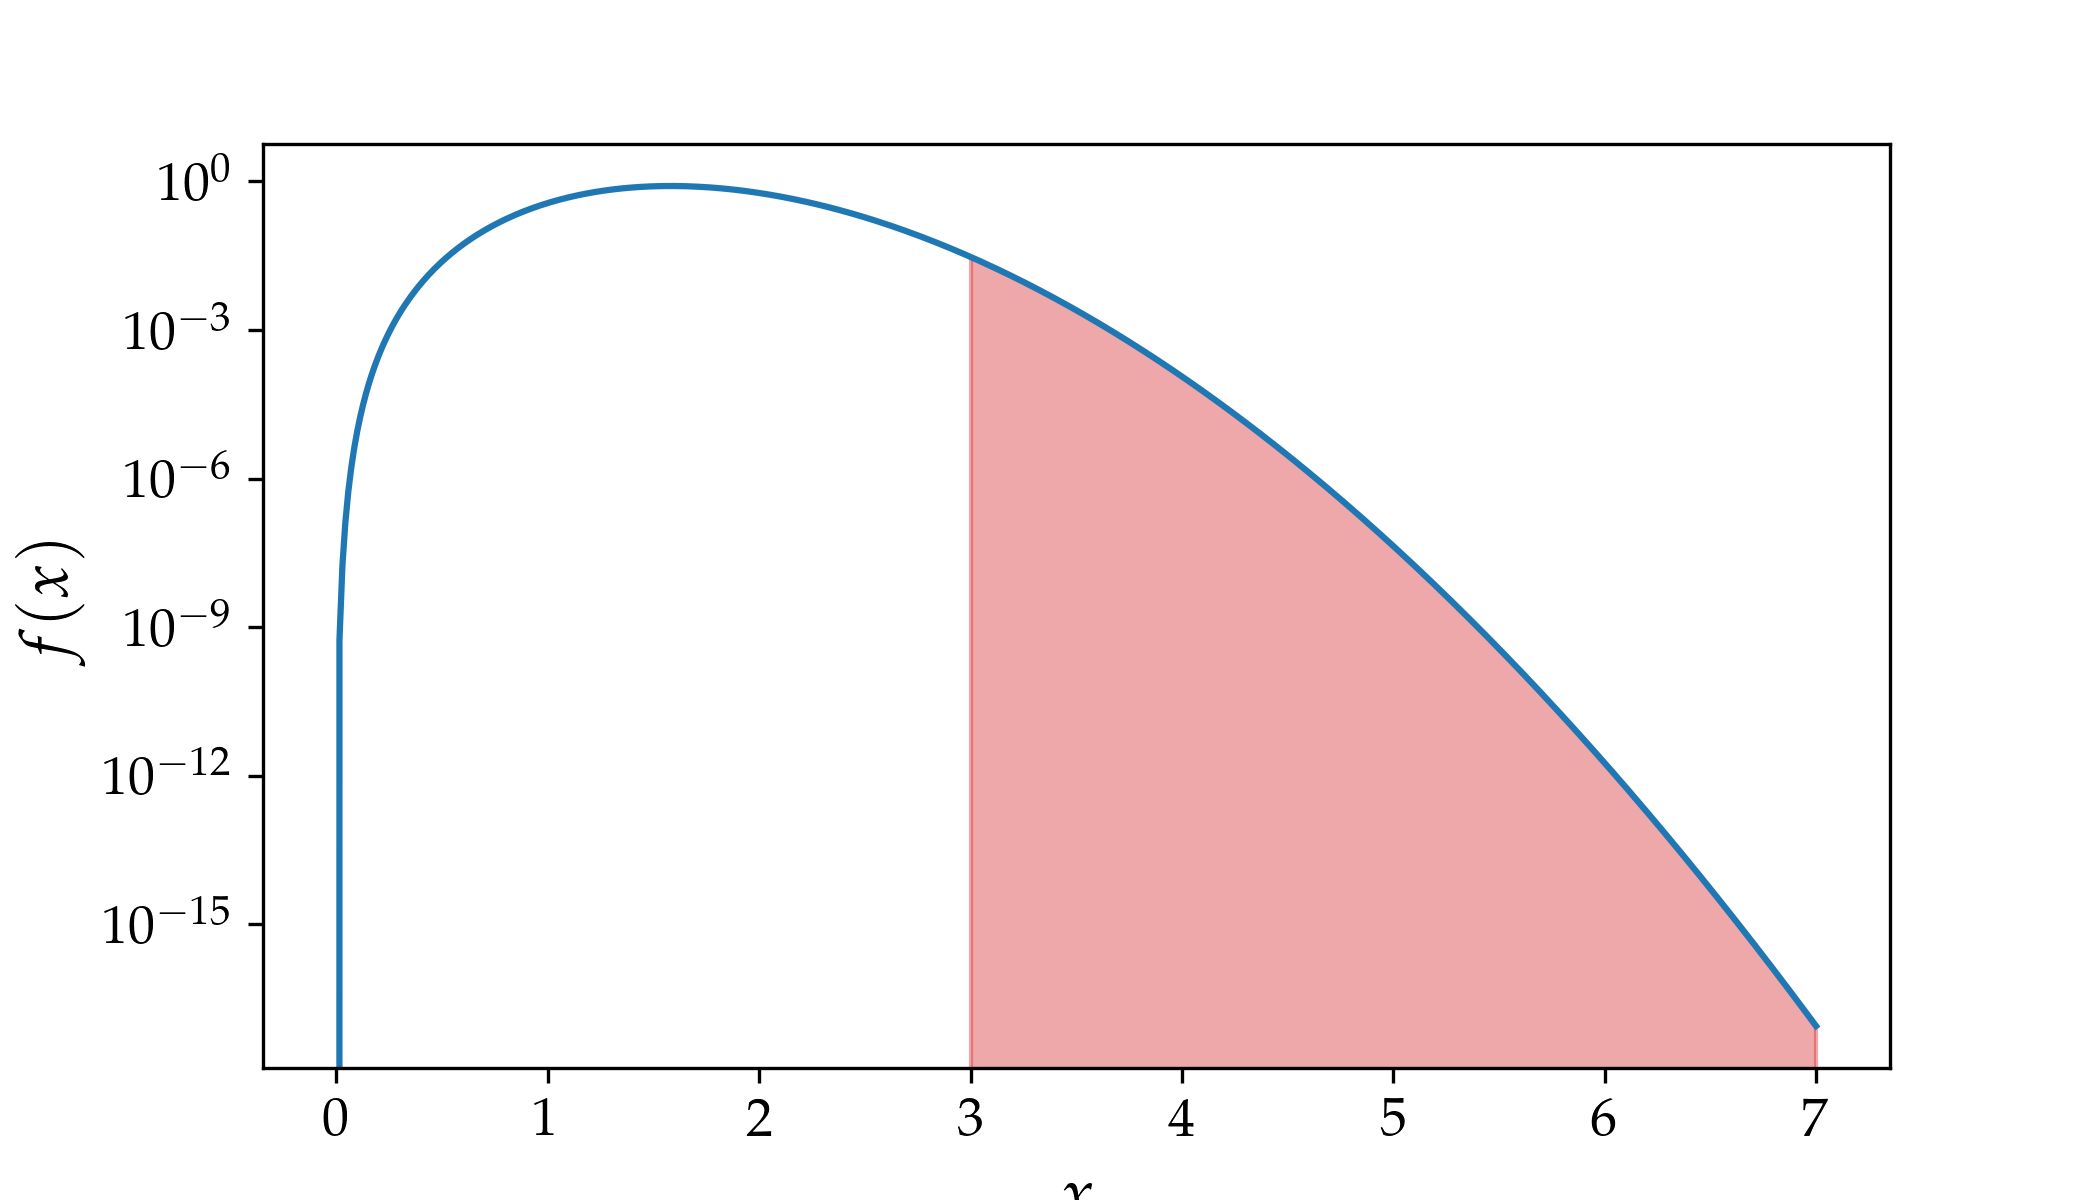
\includegraphics[width=0.7\linewidth]{images/22/func_display_part.png}
        \caption{Intervallo di valutazione della funzione.}
        \label{fig: val_func}
    \end{figure}

    In particolare si noti come il metodo risulti instabile e poco accurato: l'errore non riesce a scendere sotto l'ordine di $10^{-3}$ neanche nel punto in cui otteniamo il miglior risultato. Una figura che è ancora più esplicativa è quella relativa al confronto della convergenza dei metodi, Fig. \ref{fig: conv_mth}. Si noti la convergenza asintotica di Simpson e dei trapezi, mentre l'algoritmo della quadratura di Gauss-Hermite non è convergente, ha invece carattere oscillatorio.

    \begin{figure}[H]
        \centering
        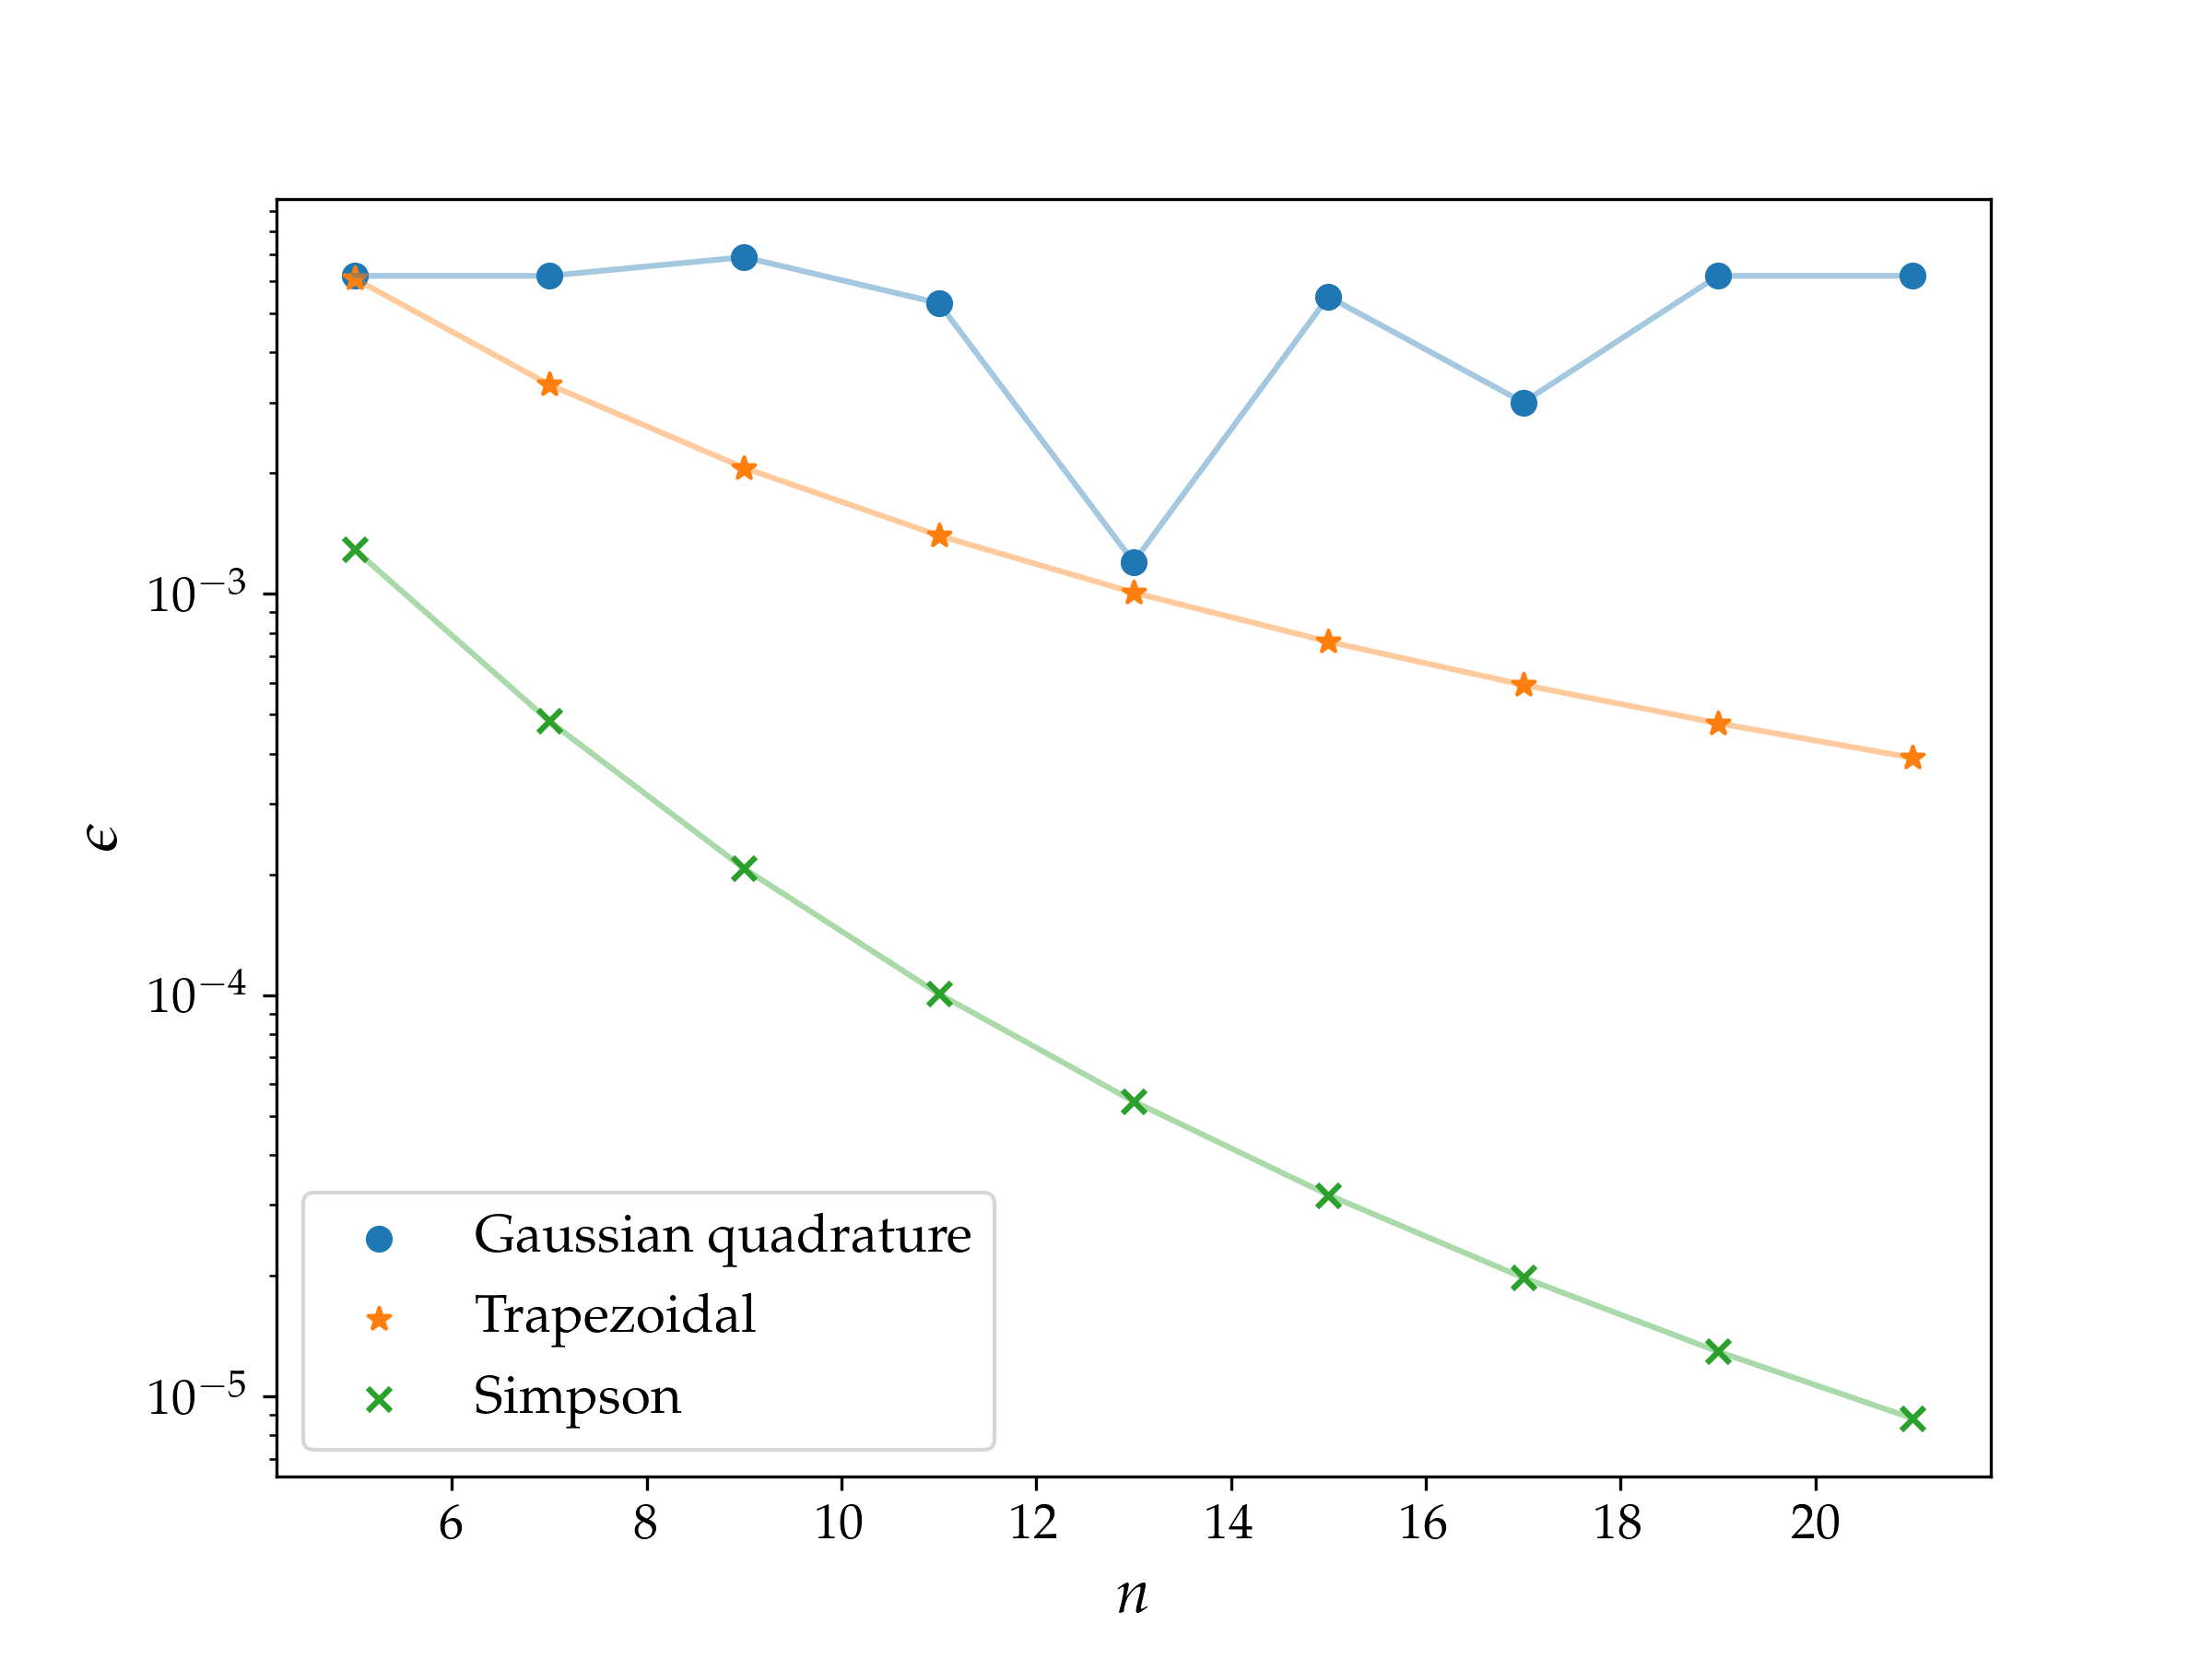
\includegraphics[width=0.7\linewidth]{images/22/confr.png}
        \caption{Confronto diretto dei tre metodi numerici per la valutazione dell'integrale $I_3$.}
        \label{fig: conv_mth}
    \end{figure}

    È anche possibile confermare l'andamento dei due metodi per precisioni maggiori, scegliendo $n$ più grandi, che invece bloccherebbero l'esecuzione del primo algoritmo. Osserviamo in Fig. \ref{fig: conv_mth_fit} come la pendenza rispecchia ciò che ci aspettiamo analiticamente, cioè una convergenza quadratica e quartica rispettivamente per la regola dei trapezi e di Simpson. 

    Si noti che nei grafici è riportata, per continuità con i confronti precedenti, la convergenza in funzione del numero di sottointervalli in cui suddividiamo il dominio. La convergenza è $O(n^p),\ p >0$ quando la osserviamo in relazione allo spacing $\delta x$, il quale è inversamente proporzionale al numero di intervalli; così spiegati gli andamenti asintotici con potenze negative.

    \begin{figure}[H]
        \centering
        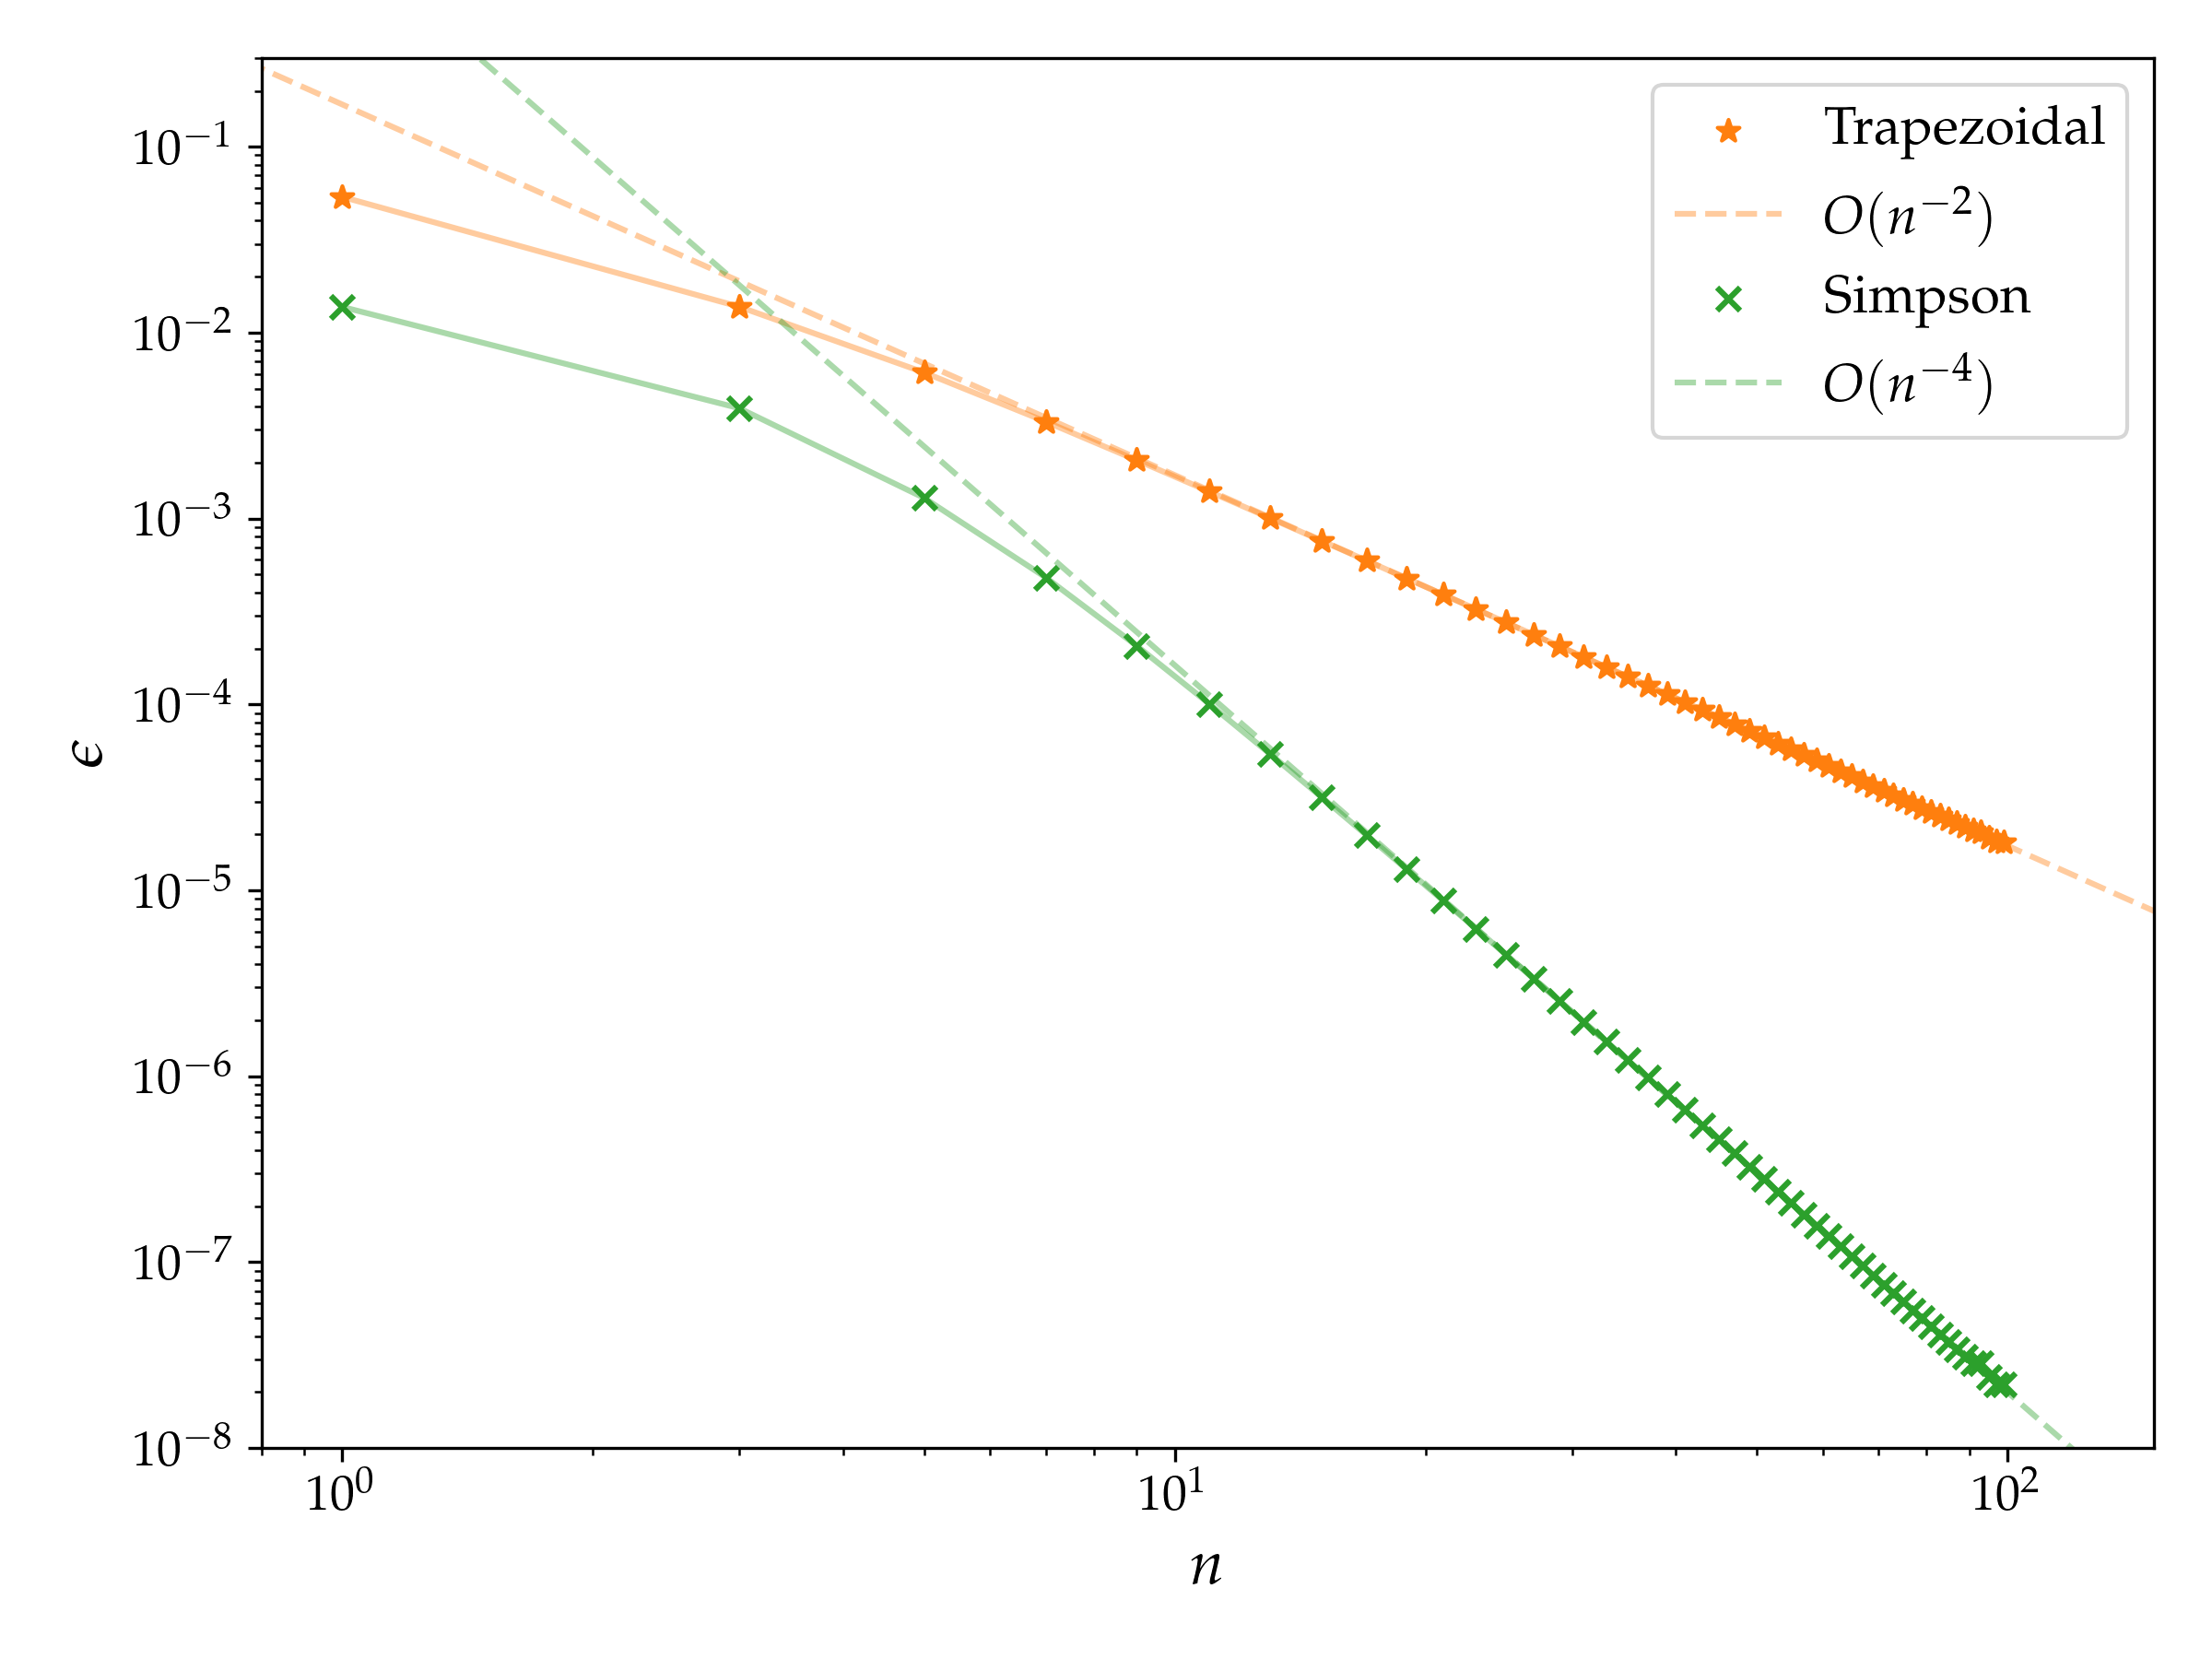
\includegraphics[width=0.7\linewidth]{images/22/confr_fit.png}
        \caption{Confronto della convergenza asintotica per i metodi dei trapezi e di Simpson per $I_3$.}
        \label{fig: conv_mth_fit}
    \end{figure}

        
\end{enumerate}

\bigskip\noindent
Infine si commenta il plot richiesto di $w_i(x_i)$: l'idea di introdurre dei pesi si riferisce alla possibilità di attribuire una importanza diversa a diversi punti di valutazione della funzione, in corrispondenza proprio dei nodi $x_i$, in funzione all'informazione che essi veicolano per calcolare il valore della funzione generale. I pesi quantificano il contributo numerico associato a ciascun nodo della quadratura e la loro distribuzione è una conseguenza delle proprietà di ortogonalità dei polinomi di Hermite.


\begin{figure}[H]
    \centering
    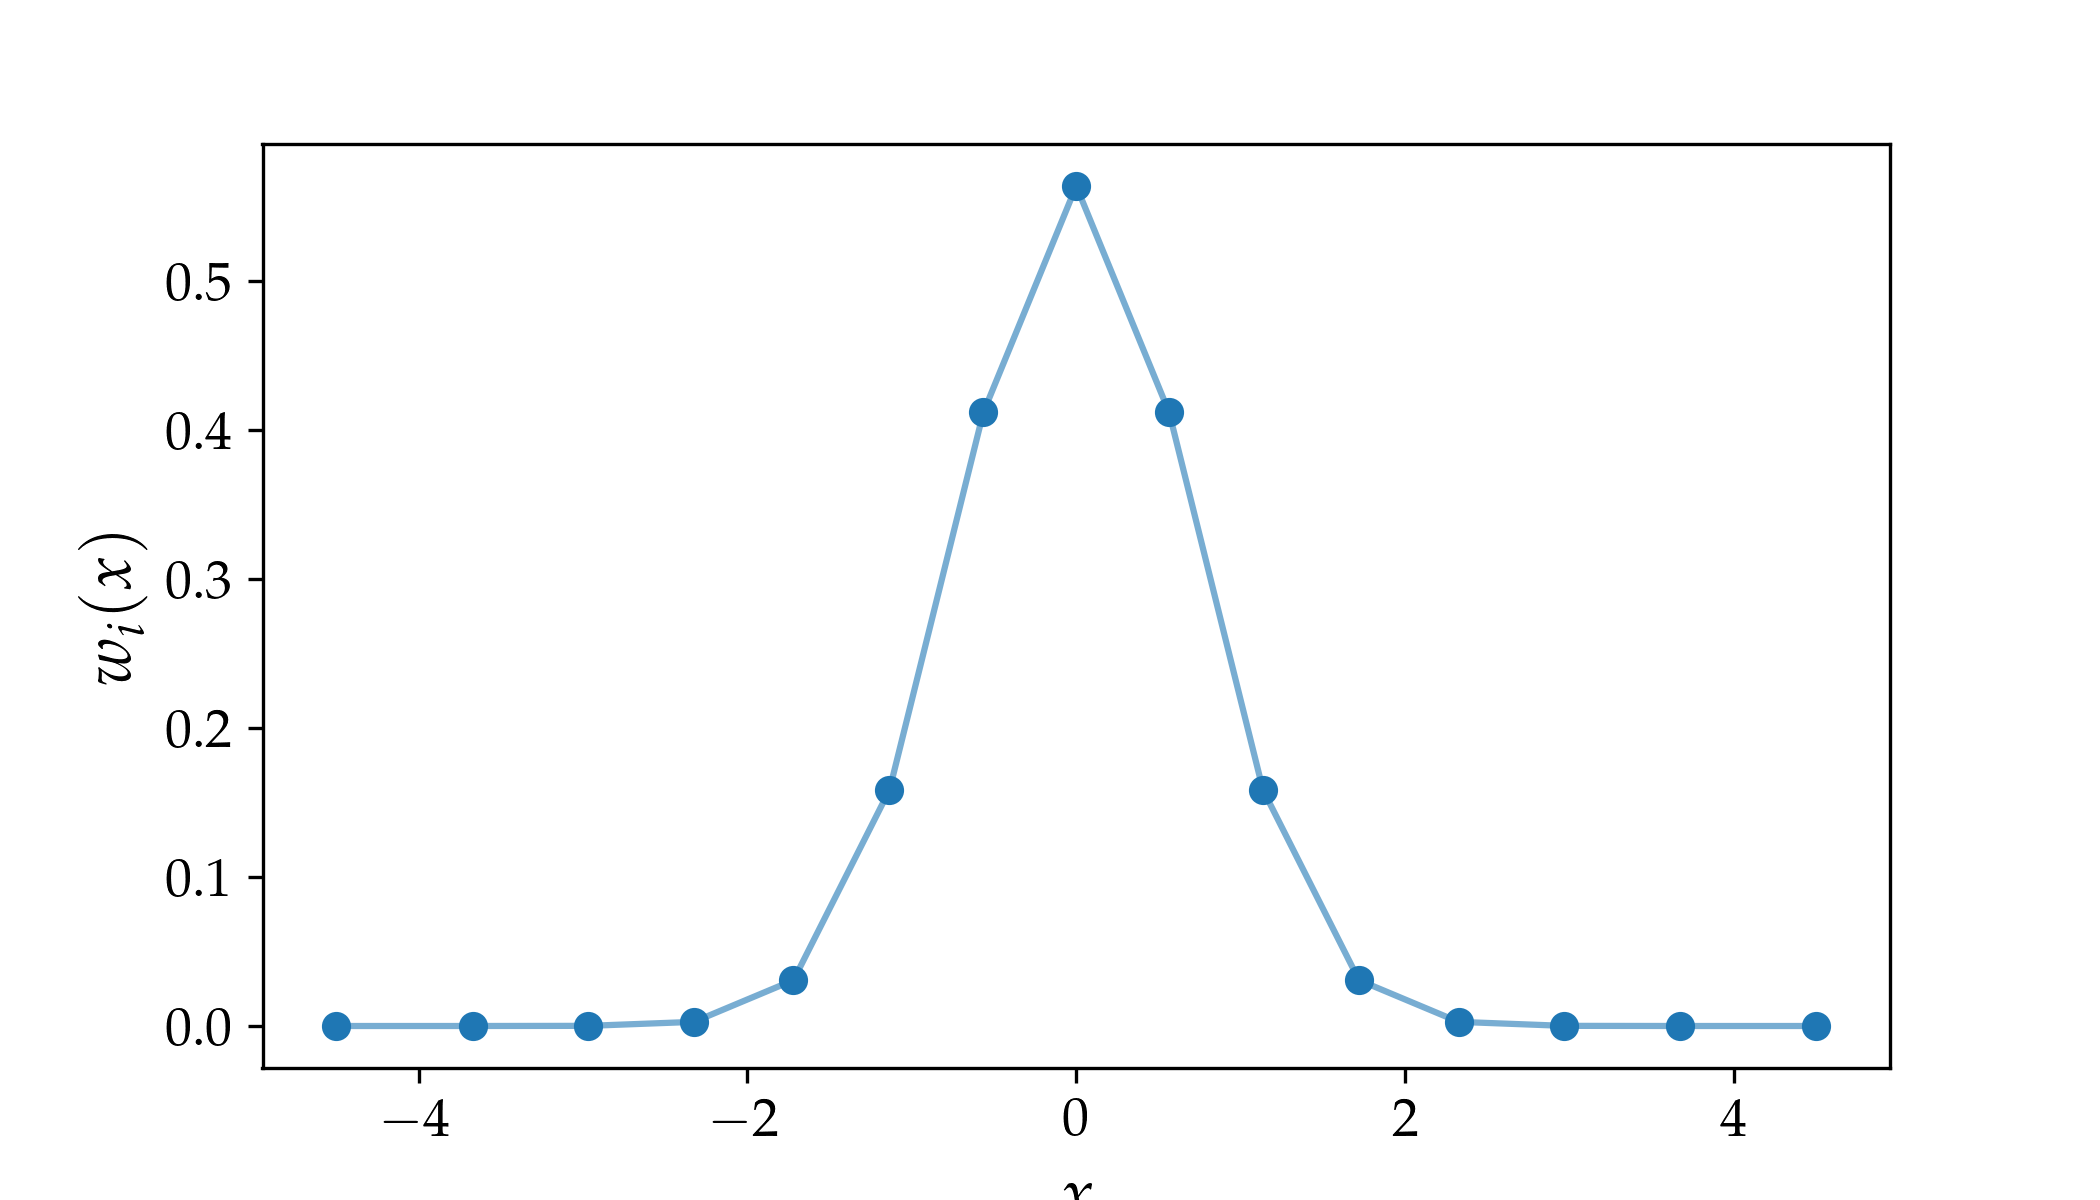
\includegraphics[width=0.7\linewidth]{images/22/weight_example.png}
    \caption{Rappresentazione dei pesi sulle i-esime radici dei polinomi di Hermite.}
    \label{fig: weight_her}
\end{figure}

\newpage








